% Balbin_Archie_W3.tex - \sysname{} Capstone Thesis
% !TEX root = Balbin_Archie_W3.tex
% NCF Capstone Format
\documentclass{research}

\usepackage{float}
\usepackage{longtable}
\usepackage{algorithm}
\usepackage{algpseudocode}
\usepackage{tikz}
\usetikzlibrary{arrows.meta,positioning,shapes.geometric}

% ── System name placeholder: change ONE line here when name is decided ──
\newcommand{\sysname}{QueuEx}

\setcounter{secnumdepth}{1}

% Subsections: no number, indented title flush with paragraph indent
\titleformat{\subsection}
  {\normalfont\normalsize\bfseries}
  {}
  {0em}
  {\hspace*{\parindent}}
\titlespacing*{\subsection}{0pt}{1.5ex plus .5ex minus .2ex}{0.8ex plus .1ex}

% Subsubsections: no number, indented title
\titleformat{\subsubsection}
  {\normalfont\normalsize\bfseries}
  {}
  {0em}
  {\hspace*{\parindent}}
\titlespacing*{\subsubsection}{0pt}{1.2ex plus .4ex minus .2ex}{0.6ex plus .1ex}

\graphicspath{{images/}}
\addbibresource{Balbin_Archie_W3.bib}

% No single line of a paragraph stranded at the top or bottom of a page.
\widowpenalty=10000
\clubpenalty=10000
\displaywidowpenalty=10000
\begin{document}

% ============================================================
% TITLE PAGE
% ============================================================
\begin{titlepage}
\centering
\vspace*{0.95in}
{\LARGE\bfseries \sysname{}: A Computer Vision-Based Smart Queue Management and
Predictive Service Delivery System\par}
\vfill
{A Senior Project\par
\medskip
Presented to the Faculty of the\par
College of Computer Studies\par
Naga College Foundation, Inc.\par
Naga City\par}
\vfill
{In Partial Fulfillment of\par
The Requirements for the Degree\par
Bachelor of Science in Computer Science\par}
\vfill
{Archie D. Balbin\par
Joshua Rovic P. Sanota\par}
\vfill
{2027\par}
\end{titlepage}

\pagenumbering{roman}
\setcounter{page}{2}
\pagestyle{empty}
\fancypagestyle{plain}{\fancyhf{}\renewcommand{\headrulewidth}{0pt}}

% ============================================================
% APPROVAL SHEET
% ============================================================
\begingroup
\small
\begin{center}
NAGA COLLEGE FOUNDATION, INC.\\
College of Computer Studies\\
City of Naga
\end{center}
\vspace{0.6em}
\begin{center}
\textbf{APPROVAL SHEET}
\end{center}
\vspace{0.6em}

\noindent This capstone research of \textbf{ARCHIE D. BALBIN} and
\textbf{JOSHUA ROVIC P. SANOTA}
entitled \textbf{``QUEUEX: A COMPUTER VISION-BASED SMART QUEUE MANAGEMENT AND
PREDICTIVE SERVICE DELIVERY SYSTEM''} was prepared and submitted in
partial fulfillment of the requirements for the degree of Bachelor of
Science in Computer Science. It has been examined and is recommended
for acceptance and approval for oral examination.

\vspace{1em}
\begin{center}
\textbf{Fritzgerald Enric T. Imperial, MIT}\\
Adviser
\end{center}

\vspace{1em}
\begin{center}
\textbf{THESIS COMMITTEE:}
\end{center}

\vspace{0.5em}
\begin{center}
\textbf{DR. ANNA LORETTA C. ROMULO}\\
Chairman
\end{center}

\vspace{0.5em}
\begin{minipage}{0.45\textwidth}
\centering
\textbf{DR. RONEL B. SIMON}\\
Panel Member
\end{minipage}
\hfill
\begin{minipage}{0.45\textwidth}
\centering
\textbf{RONALD O. BALDEMORO, MIT}\\
Panel Member
\end{minipage}

\vspace{0.7em}
\begin{center}
\textbf{LIELA B. GARDOSE, MBA}\\
Panel Secretary
\end{center}

\vspace{1em}
\begin{center}
\textbf{PANEL OF EXAMINERS}
\end{center}

\noindent Approved by the Committee on Pre-Oral Examination on
\underline{\hspace{4cm}}.

\vspace{0.5em}
\begin{center}
\textbf{DR. ANNA LORETTA C. ROMULO}\\
Chairman
\end{center}

\vspace{0.5em}
\begin{minipage}{0.45\textwidth}
\centering
\textbf{DR. RONEL B. SIMON}\\
Panel Member
\end{minipage}
\hfill
\begin{minipage}{0.45\textwidth}
\centering
\textbf{RONALD O. BALDEMORO, MIT}\\
Panel Member
\end{minipage}

\vspace{0.8em}
\noindent Accepted and approved in partial fulfillment of the
requirements for the degree of Bachelor of Science in Computer Science.

\vspace{0.7em}
\begin{center}
\textbf{DR. ANNA LORETTA C. ROMULO}\\
Dean
\end{center}
\endgroup

\newpage

% ============================================================
% SECRETARY'S CERTIFICATION
% ============================================================
\begin{center}
NAGA COLLEGE FOUNDATION, INC.\\
College of Computer Studies\\
City of Naga
\end{center}
\vspace{1.5em}
\begin{center}
\textbf{SECRETARY'S CERTIFICATION}
\end{center}
\vspace{1.5em}

\noindent This capstone research of \textbf{ARCHIE D. BALBIN} and
\textbf{JOSHUA ROVIC P. SANOTA}
entitled \textbf{``QUEUEX: A COMPUTER VISION-BASED SMART QUEUE MANAGEMENT AND
PREDICTIVE SERVICE DELIVERY SYSTEM''} was prepared and submitted in
partial fulfillment of the requirements for the degree of Bachelor of
Science in Computer Science. It has been examined and is recommended
for acceptance and approval for oral examination.

\vspace{2em}
\begin{center}
\textbf{LIELA B. GARDOSE, MBA}\\
Secretary
\end{center}

\newpage

% ============================================================
% EDITOR'S CERTIFICATION
% ============================================================
\begin{center}
NAGA COLLEGE FOUNDATION, INC.\\
College of Computer Studies\\
City of Naga
\end{center}
\vspace{1.5em}
\begin{center}
\textbf{EDITOR'S CERTIFICATION}
\end{center}
\vspace{1.5em}

\noindent This capstone research of \textbf{ARCHIE D. BALBIN} and
\textbf{JOSHUA ROVIC P. SANOTA}
entitled \textbf{``QUEUEX: A COMPUTER VISION-BASED SMART QUEUE MANAGEMENT AND
PREDICTIVE SERVICE DELIVERY SYSTEM''} was prepared and submitted in
partial fulfillment of the requirements for the degree of Bachelor of
Science in Computer Science. It has been examined and is recommended
for acceptance and approval for oral examination.

\vspace{2em}
\begin{center}
\textbf{}\\
Editor
\end{center}

\newpage

% ============================================================
% ACKNOWLEDGMENT
% ============================================================
\begin{center}
\textbf{ACKNOWLEDGMENT}
\end{center}
\vspace{1.5em}

\noindent The researchers express their sincere gratitude to
Fritzgerald Enric T. Imperial, MIT, their adviser, for his guidance,
technical advice, and patience throughout the development and writing
of this capstone research.

\newpage

% ============================================================
% ABSTRACT
% ============================================================
\begin{center}
{\large\textbf{Abstract}}
\end{center}
\vspace{1.5em}

\noindent
\begin{tabular}{p{0.30\textwidth} p{0.63\textwidth}}
\textbf{Title:} &
  \textbf{\sysname{}: A Computer Vision-Based Smart Queue Management and
  Predictive Service Delivery System} \\[0.6em]
\textbf{Researcher:} &
  Archie D. Balbin and Joshua Rovic P. Sanota \\[0.6em]
\textbf{Type of Document:} &
  Unpublished Undergraduate Capstone Research (2027) \\[0.6em]
\textbf{Host/Accrediting School:} &
  Naga College Foundation, Inc. \\[0.6em]
\textbf{City:} & Naga City \\[0.6em]
\textbf{Region:} & Region V \\[0.6em]
\textbf{Year of Completion:} & 2027 \\[0.6em]
\textbf{Adviser:} & Fritzgerald Enric T. Imperial, MIT \\[0.6em]
\textbf{Keywords:} &
  Queue management, computer vision, YOLOv8, person re-identification,
  predictive analytics, FastAPI, printer-agnostic ticket protocol, QR code,
  JWT, M/M/c model, Holt's double exponential smoothing \\
\end{tabular}

\vspace{2em}

\noindent Queueing in many campus service offices is still handled by
staff observation, manual numbering, and verbal updates at the counter.
During enrollment, payment, and clearance periods, students often do
not know how far they are from service, while staff must estimate the
line from what they can see at the counter. \sysname{} was built as a
capstone prototype for that office setting. It combines a YOLOv8n
detector, OpenCV camera processing, automatic queue-number assignment,
ticket issuance, and short-horizon wait-time forecasting. The prototype
runs the camera detector separately from the FastAPI backend: the
detector sends
tracked-person metadata, duplicate-filtered detections, crowd counts,
and annotated snapshots, while the backend confirms entrants inside a
calibrated queue zone before issuing a number. Confirmation uses a
candidate window, motion checks, track-ID remapping, and a hybrid
appearance-spatial re-entry rule so that brief exits from the camera
view do not immediately produce duplicate queue tickets. \sysname{} also
uses a printer-agnostic ticket payload containing the queue number, QR
link, short code, and JSON Web Token (JWT), which can be rendered as a
thermal ticket in deployment or as a PDF ticket in the prototype build.
Queue records are stored in MySQL, students can check ticket status
from a mobile client, and staff can monitor live snapshots, pending-link
alerts, counter actions, analytics, and forecasts through the dashboard.
The forecasting component reports the current estimated wait time and
5-, 15-, and 30-minute projections using an M/M/c baseline, local trend
projection, Holt's double exponential smoothing, and a mean-reversion
adjustment. The Naga College Foundation, Inc.\ (NCF) prototype is
evaluated through queue assignment accuracy, re-identification
reliability, ticket and token validation, prediction error using MAE
and MAPE, system latency, and user satisfaction.

\newpage

% ============================================================
% TABLE OF CONTENTS / FIGURES / TABLES
% ============================================================
\tableofcontents
\newpage
\listoffigures
\newpage
\listoftables
\newpage

% ============================================================
% CHAPTER 1: INTRODUCTION
% ============================================================
\fancypagestyle{plain}{\fancyhf{}\fancyhead[R]{\thepage}\renewcommand{\headrulewidth}{0pt}}
\pagenumbering{arabic}
\pagestyle{fancy}
\chapter{Introduction}

\section{Background of the Study}
\label{cr:background}

Queue management inefficiency is a recognized challenge in service delivery organizations worldwide. Research from banking, healthcare, government service desks, and academic institutions consistently documents that manual queue processes cannot provide real-time status visibility, accurate wait-time estimates, or adaptive counter management when demand increases rapidly~\cite{nair2025survey,batcharo2025smart,yifter2023modeling}. As organizations in various sectors have introduced automated queue systems—which combine digital ticketing, camera-based monitoring, and predictive analytics—the operational gap between manual and automated queue management has widened~\cite{rashid2023smartqueue,zou2026customer}. In these settings, the absence of automated observation and prediction leaves both service staff and clients without the information needed to manage or navigate the service flow efficiently.

In the Philippines, this gap is visible across higher education institutions (HEIs). Enrollment, payment, and clearance cycles bring concentrated student arrivals to service windows within compressed periods, creating queue conditions that manual staff management cannot easily absorb. Philippine studies document the persistence of long enrollment queues and the operational pressure that rising student volumes place on service windows~\cite{concepcion2026smart,mallari2022clique,rrlcomp023automatedenrollmentqueueing,rrlcomp025lineuclmenhancing}. Existing Philippine HEI queue solutions primarily address web-based ticketing and appointment-booking rather than real-time passive observation of student arrivals at service areas.

At Naga College Foundation, Inc.\ (NCF), informal accounts from students and service staff indicate that wait times during enrollment, payment, and clearance periods can become substantial, with congestion most pronounced during the first weeks of each semester. Enrollment, cashiering, and library services are separate offices, but students often experience them as one connected process, so a delay at one window affects the next transaction the student must complete. This pattern, combined with the absence of a real-time queue display and manual recording of transaction order, reflects the same kind of service delivery inefficiency that the literature identifies as a recurring issue in Philippine HEIs. The Commission on Higher Education recognizes accessibility and efficient service delivery as indicators of institutional quality~\cite{ched2022}; for this reason, improving queue visibility is treated in this study as part of improving the student service experience, not merely as a counter-management task.

Conventional queue systems are useful once a student has requested a
number or once staff have encoded the transaction. Their limitation is
that they normally begin after the office has already recognized the
arrival. They can store issued tickets, but they do not usually observe
the service area, confirm new arrivals from a camera view, reduce
duplicate queue entries, or estimate near-term changes in the line. The
gap is therefore not only ticket issuance; it is the missing link among
arrival detection, staff monitoring, student status access, and
prediction.

\sysname{} responds to this gap through a camera-connected queue
management prototype for campus service offices. Its central mechanism
is identification rather than counting: a student enrols a face
signature once from their own phone, requests a place in the queue when
they need one, and is then issued a queue number automatically when the
queue-zone camera recognizes them, with no staff encoding and no manual
entry at the counter. Detection establishes that somebody is present;
recognition establishes \emph{who}, which is what allows a number to be
issued to a named student rather than merely added to a count.

The detection stage uses YOLOv8n and OpenCV to locate persons inside a
defined queue zone. YOLO is appropriate for this use case because it
performs object detection in a single network pass~\cite{redmon2018}.
YOLOv8n was selected because it is light enough for prototype-grade
hardware while still supporting ByteTrack-based persistent
tracking~\cite{zhang2022bytetrack} and stable deployment
tooling~\cite{jocher2023,wang2025lightweight}. Newer YOLO variants,
including YOLOv11 and YOLOv12, introduce architectural
improvements~\cite{jocher2024yolo11,tian2025yolov12}; however, this
study prioritizes stable single-class person detection in a controlled
queue zone over marginal accuracy gains that may require more
computing resources. The selection therefore reflects the constraints
of the prototype environment rather than a general claim that YOLOv8n
is superior in all settings.

Identification is performed on the face. Each detected person's face is
converted to a compact numeric embedding, which is compared against the
signatures of enrolled students. A match is accepted only when it clears
an absolute similarity threshold \emph{and} leads the next-best candidate
by a stated margin, so that a face resembling two enrolled students
equally is refused rather than assigned to whichever scored marginally
higher. Refusal is the safe outcome: the person remains pending and a
member of staff resolves the case. The same rule allows people who have
not enrolled to pass through the queue zone without ever being
identified.

\sysname{} further extends detection with duplicate filtering, candidate
confirmation, and face-based re-entry matching so that queue records
remain consistent when people move or briefly leave the camera frame. The
ticket component is printer-agnostic: each confirmed queue entry
receives a queue number, a short code, a QR link, and a JSON Web Token
(JWT) for status checking. At the service counter, this payload can be
printed on thermal paper. For the prototype runs, it is rendered as a
downloadable PDF, allowing the ticket identity and validation flow to
be tested without making the printer hardware the focus of the study.

Beyond ticket generation, \sysname{} connects the detector, queue
records, staff dashboard, and prediction module through a FastAPI-based
backend and MySQL database. The prediction module reports current,
5-minute, 15-minute, and 30-minute wait-time estimates using queuing
logic and short-term forecasting. For NCF, the prototype is intended to
answer a concrete operational question: whether a camera-fed queue
record can give staff and students a clearer view of the line before a
manual counter update is made.

The Review of Related Literature therefore examines the technologies
and concepts that support each part of the problem identified above.
Computer vision and YOLO literature address automated queue observation;
face-recognition literature addresses the identification step on which
automatic number issuance depends, together with the open-set
requirement that unenrolled people be refused rather than matched to the
nearest enrolled face; queue management literature explains ticketing and
identity maintenance; and forecasting literature supports the wait-time
estimates needed for staff decision-making.

\section{Review of Related Studies}
\label{cr:rrl}

\subsection{Computer Vision for Real-Time Person Detection}
Recent computer-vision work shows why camera-based queue observation is
technically feasible. Sindagi and Patel~\cite{sindagi2018survey}
surveyed CNN-based crowd counting and density-estimation methods,
noting the move from earlier scale-limited approaches to models that
handle occlusion, complex scenes, and dense groups more reliably.
One-stage detectors such as YOLO are relevant to this study because
they process a frame quickly enough for live monitoring~\cite{redmon2018}.
Terven et~al.~\cite{terven2023yolo} trace YOLO's development from
YOLOv1 through YOLOv8 and YOLO-NAS, with attention to the
accuracy-speed tradeoff in each generation. Wang
et~al.~\cite{wang2025lightweight} more recently proposed a
YOLOv8n-derived person detector for edge-device surveillance, which
supports the decision to use a lightweight YOLOv8n base in the
\sysname{} prototype.

Because \sysname{} uses a camera, privacy is treated as a design
constraint rather than an afterthought. Padilla-Lopez
et~al.~\cite{padillalopez2015privacy} survey visual privacy protection
methods such as camera-level anonymization, selective scrambling, and
aggregate-only transmission. In \sysname{}, this concern is reflected in
the decision to work with derived data: bounding boxes for detection and
face embeddings for identification, neither of which is an image. No raw
video, camera frame or enrolment photograph is stored or transmitted.

Real-time people counting using YOLOv8 has been validated across varied
environments. An IEEE conference publication~\cite{rrlcomp001realtimepeople}
demonstrates a people-counting pipeline built on YOLOv8 object detection,
confirming that the model's speed and accuracy are sufficient for real-time
counting tasks without specialized hardware. In a campus-surveillance
context, Cheng et~al.~\cite{rrlcomp016sgstyolov8improved} propose
SGST-YOLOv8, a lightweight modification of YOLOv8 designed for real-time
target detection on campus, showing that architectural adjustments can
reduce inference time while maintaining detection accuracy on small,
partially occluded persons. A comparative evaluation~\cite{rrlcomp019evaluatingyolov8yolov11}
assesses both YOLOv8 and YOLOv11 for real-time person detection in crowded
environments, finding that YOLOv8 offers mature tooling and tracking
integration that make it particularly practical for deployment.

People-counting research has also explored camera-based monitoring of
public and semi-public spaces. A 2023 IEEE
publication~\cite{rrlcomp031peoplecountingpublic} presents a
deep-learning system for counting and tracking people in public spaces,
combining object detection with tracking to produce accurate density
estimates over time. A study in the Journal of
Imaging~\cite{rrlcomp032visionpeoplecounting} applies vision-based
counting and tracking to urban environments, addressing challenges such
as varying crowd density, overlapping bounding boxes, and perspective
distortion. Deep learning video analysis has also been applied to
visitor detection and tracking in real-world deployments~\cite{rrlcomp033deeplearningvideo},
demonstrating operation under lighting variability and occlusion
conditions typical of live camera feeds.

Crowd anomaly detection is a closely related area whose findings
inform the design of queue-zone filtering. A Springer
review~\cite{rrlcomp034deepcrowdanomaly} surveys the state of deep
crowd anomaly detection, identifying temporal context modelling as an
open challenge. A survey in Personal and Ubiquitous
Computing~\cite{rrlcomp042surveydeeplearning} reviews distributed crowd
anomaly detection approaches for secure video surveillance, noting the
trade-off between model complexity and latency in live systems. More
recently, a Springer study~\cite{rrlcomp043enhancedframeworkreal}
proposes a YOLOv8-based framework for dense-crowd abnormal-behaviour
detection, showing that the detector can identify individual persons
even at high density when the detection zone and confidence thresholds
are tuned appropriately.

Architectural advances in YOLOv8 have produced lighter and more
precise detectors. Liu et~al.~\cite{rrlcomp091improvedyolov8lightweight}
present an improved YOLOv8 with a lightweight attention mechanism for
cross-scale feature fusion, achieving better small-target recall with a
reduced parameter count. Varghese and
Sambath~\cite{rrlcomp092yolov8novelobject} evaluate YOLOv8 as a novel
detection algorithm, documenting its enhanced performance and robustness
relative to earlier YOLO generations. A deep-learning
framework~\cite{rrlcomp020frameworkpedestrianattribute} for pedestrian
attribute recognition co-processes bounding-box features and visual
attributes, a method relevant to any application requiring person
classification beyond simple localization.

Privacy constraints apply equally to systems operating in educational
settings. An IEEE publication~\cite{rrlcomp013lowlatencyvideo} presents
a low-latency video anonymization pipeline that protects privacy without
preventing crowd detection. Bonetto
et~al.~\cite{rrlcomp021privacypreservingsurveillance} describe
privacy-preserving surveillance as an edge service using lightweight
video protection schemes that process and anonymize footage locally,
removing the need to transmit identifiable images. A survey in Applied
Sciences~\cite{rrlcomp022perceptionrisksusefulness} examines user
perceptions of smart video surveillance, finding that acceptance depends
on transparency about data use and the absence of facial recognition.
An IEEE study~\cite{rrlcomp040deeplearninggdpr} further implements
GDPR-compliant privacy safeguards in surveillance video using deep
learning to suppress personal identifiers before storage.

Detection in a queue is not a per-frame problem. A number must stay with
the same person across frames, which requires a tracker to carry
identity forward, and the literature pairs detection with tracking
accordingly. Person detection using YOLOv8 with DeepSORT
tracking~\cite{rrlcomp003persondetectionproposed} demonstrates the
combination on the person class specifically, while pedestrian tracking
studies based on YOLOv8 with
OC-SORT~\cite{rrlcomp017multiobjectpedestrian} and with an improved
association stage~\cite{rrlcomp018multiobjectivepedestrian} report
gains in identity consistency under the crowding and partial occlusion
typical of pedestrian scenes. YOLO has also been paired with a sliding
innovation filter for joint detection and
tracking~\cite{rrlcomp098objectdetectiontracking}, and with centroid
tracking for real-time directional
monitoring~\cite{rrlcomp099realtimewrong}, the latter illustrating how
a zone-based rule can be layered on top of ordinary tracking output in
the way \sysname{} applies a queue zone.

The association step itself rests on motion prediction. Kalman filtering
remains the standard mechanism, and recent work refines it in ways that
matter for a fixed indoor camera: adaptive formulations for real-time
visual tracking~\cite{rrlcomp061adaptivekalmanfilter}, unscented
variants for non-linear
motion~\cite{rrlcomp062achievingadaptivevisual}, and reliability-weighted
object information to resist drift when observations become
unreliable~\cite{rrlcomp063robustvisualtracking}. Studies of
bounding-box dynamics and noise covariance
modelling~\cite{rrlcomp064boundingboxdynamics} show that the box itself
is a noisy measurement, which is the justification for the smoothing
applied before any box in \sysname{} is used for a zone decision.

Overlap handling is the remaining requirement, because a detector
returning several boxes for one person would otherwise inflate a queue
count. Non-maximum suppression is the standard remedy, and its
limitations in crowded scenes are well documented. Work on where
suppression belongs in a tracking
pipeline~\cite{rrlcomp046nonmaximumsuppression} argues for applying it
later than is conventional; multi-attribute
NMS~\cite{rrlcomp047multiattributenms} targets pedestrian detection in
crowds specifically, where genuine neighbouring people produce high
mutual overlap; soft suppression
schemes~\cite{rrlcomp086enhancednmsdetection} decay rather than
eliminate competing boxes; spatial
correlation~\cite{rrlcomp089spatialnonmaximum} and adaptive
thresholding for small
objects~\cite{rrlcomp090adaptiveiouthresholding} adjust the overlap
criterion to the scene rather than fixing it in advance. These findings
inform the overlap and duplicate-suppression gates described in
Chapter~3, which operate on the same principle that a fixed global
threshold is a poor fit for a zone where people legitimately stand close
together.

\subsection{Face Recognition and Open-Set Identification}

Detection and tracking establish that a person is present and keep them
distinct from their neighbours, but neither can say who that person is.
The revised \sysname{} design requires exactly that: a queue number is
issued to a named enrolled student, so the system must identify rather
than merely count. The literature on deep face recognition provides both
the representation used for that step and the decision framework that
governs when an identification may be trusted.

\textbf{Faces as embeddings.} Modern face recognition does not compare
images directly. Schroff et~al.~\cite{schroff2015facenet} established
the approach \sysname{} follows, training a network to map a face into a
compact vector space in which distance corresponds to identity, so that
recognition, verification and clustering all reduce to distance
comparisons between vectors. The practical consequence for a deployed
system is that identity can be stored as a short numeric vector rather
than as a photograph, since the mapping runs in one direction and the
face cannot be reconstructed from the vector. Surveys of the field
confirm that this embedding formulation, rather than any particular
network architecture, is what unified the
discipline~\cite{wang2021deepfacesurvey,facesurvey2022}, and they trace
the remaining variation to how the embedding space is trained and how
its distances are thresholded.

\textbf{Margins in the representation.} The refinement that matters for
this study concerns how such an embedding space is shaped during
training. Liu et~al.~\cite{liu2017sphereface} began the line of work by
constraining embeddings to a hypersphere and imposing an angular margin
between identity classes. Wang et~al.~\cite{wang2018cosface} recast the
idea as a large-margin cosine loss that explicitly widens the separation
between identities while tightening each identity's own cluster, and Deng
et~al.~\cite{deng2019arcface} extended it with an additive angular
margin, producing the ArcFace formulation used by the recognition model
in \sysname{}. Later refinements attach magnitude to sample quality so
that ambiguous faces are pushed away from class
centres~\cite{meng2021magface}, or reformulate the objective as binary
classification to simplify training at
scale~\cite{wen2021sphereface2}. The shared insight across all of them
is that a recognition system becomes reliable not by scoring similarity
more precisely but by enforcing a margin between identities. \sysname{}
applies the same principle a second time, at the decision stage rather
than the training stage: a margin in the representation is what makes
identities separable, and a margin in the decision is what determines
whether a particular comparison is separable enough to act on.

\textbf{Locating the face before recognising it.} Recognition assumes an
aligned face crop, which a person detector does not provide. Deng
et~al.~\cite{deng2020retinaface} introduced the single-shot detector and
five-point alignment stage that \sysname{} relies on through the same
toolkit, jointly predicting the bounding box and the landmarks used to
normalise pose before the embedding is computed. Because detection runs
on every frame while recognition runs only on confident crops, the
detector's cost dominates in practice, and work on lightweight detection
for embedded deployment~\cite{embeddedfacedetect2025} reports the
inference-time reductions that make CPU-only operation viable.

\textbf{Recognition on modest hardware.} A campus prototype cannot
assume a GPU. Chen et~al.~\cite{chen2018mobilefacenets} showed that a
face-verification network under one million parameters can approach the
accuracy of models hundreds of times larger, and the resulting
MobileFaceNet architecture is the recognition model \sysname{} runs.
Subsequent work has pushed the same direction through neural
architecture search and knowledge
distillation~\cite{pocketnet2022} and through architectures designed
specifically for edge inference~\cite{edgeface2024}. The relevance to
this study is that recognition accuracy and deployability are no longer
in tension at the scale of a single service office.

\textbf{Deciding when not to answer.} A campus service office is an open
environment: most people who pass the camera are not enrolled, and a
recognizer that always returns its closest match will name them anyway.
Scheirer et~al.~\cite{scheirer2013openset} formalised this as open-set
recognition, distinguishing it from the closed-set assumption that every
probe belongs to some known class, and argued that a usable system must
be able to reject. Günther et~al.~\cite{gunther2017opensetface} applied
the requirement directly to faces, showing that open-set identification
must handle both subjects who are known to be uninteresting and
identities never seen before, and that rejection performance is a
distinct quantity from ranking accuracy. These two works supply the
justification for the acceptance rule in \sysname{}: an absolute
similarity threshold establishes that a face resembles a known student,
and a required margin over the runner-up establishes that it resembles
one student distinctly, with refusal as the defined outcome when either
condition fails. Later treatments of open-set identification frame the
problem the same way, as a decision about whether the gallery contains
the probe at all rather than which gallery entry ranks
highest~\cite{indexofmax2020}.

\textbf{Measuring a recognizer that is allowed to refuse.} Because
refusal is a legitimate outcome, evaluation cannot reduce to a single
accuracy figure. Biometric practice reports the trade-off between false
matches and false non-matches across operating points, and recent work
argues that the error rate at a fixed operating point, rather than an
aggregate such as area under the curve or equal error rate, is what
characterises a deployed system~\cite{operatingpoint2026}. This study
adopts that stance, reporting scores and margins at the thresholds
actually in force. Two further findings shape what such figures mean.
Large-scale testing has established that accuracy is not uniform across
demographic groups~\cite{grother2019frvt}, which is reason to treat a
threshold calibrated on one population as provisional elsewhere. And
image quality predicts recognition outcome strongly enough to be
estimated before matching is
attempted~\cite{terhorst2020serfiq,boutros2023crfiqa}, which is why a
detector-confidence gate precedes the embedding step in \sysname{}.
Occlusion is the clearest instance of that dependence, with accuracy
degrading measurably when part of the face is
covered~\cite{maskedreview2025}.

\textbf{Threats specific to face-based entitlement.} A system that
issues something of value on recognition invites two attacks the
literature treats separately. A presentation attack substitutes a
photograph or replay for a live face, and the countermeasures form their
own research area~\cite{yu2024antispoofing}; \sysname{} does not
implement liveness detection, which is stated as a limitation rather
than claimed as solved. A stored template is the second exposure, since
a biometric cannot be reissued once compromised, and template-protection
schemes apply non-invertible transformations so that a leaked record
cannot be matched back to a person~\cite{rathgeb2021templateprotection}.
The present build relies on the non-invertibility of the embedding
itself together with access control, which is weaker than a dedicated
protection scheme and is recorded as such.

\textbf{Deployment in educational settings.} Face recognition is already
in routine institutional use for attendance. Patel
et~al.~\cite{patel2025classroomcctv} report a classroom attendance
system built on existing CCTV infrastructure, confirming both the
feasibility of recognition from ordinary cameras and the operational
appeal of removing a manual recording step, and transfer-learning
approaches report comparable results on modest
datasets~\cite{transferattendance2021}. Campus access
management~\cite{campusaccess2024} extends the same capability from
recording presence to granting entry, which is closer to the present
case because a decision follows the recognition.

The closest precedent is Handaga et~al.~\cite{handaga2019queue}, who
adopted face recognition specifically to remove the queue that formed
when students recorded attendance one at a time. Their motivation is the
same as this study's: the manual step, not the record, is what consumes
time. The difference is what the recognition produces. Their system
marks a student present; \sysname{} issues a service entitlement, a
queue number that determines when that student is served. Issuing an
entitlement raises the cost of a wrong identification from a mistaken
attendance record to a misallocated place in a line, which is the reason
this study treats the refusal rule, rather than the recognition rate, as
its central design question.

\textbf{Proportionality.} Because face data is biometric, the decision to
deploy is not purely technical. Negri
et~al.~\cite{negri2024deploy} propose a framework for assessing whether
the use of a face recognition system is proportionate to its purpose in a
given real-world setting. Regulatory analysis points the same way:
assessments of the European Union's AI Act treat biometric
identification as a high-risk application requiring transparency and
human oversight rather than prohibiting it
outright~\cite{aiactbiometric2025}, and public-opinion research finds
that acceptance depends heavily on whether the deployment is
consent-based and auditable~\cite{remotebiometric2024}. Applied to this
study, the relevant proportionality argument is that enrolment is
voluntary and student-initiated, that recognition is confined to a
marked queue zone and to students who have separately requested service,
that unenrolled persons are refused rather than identified, and that no
photograph is retained. Section~\ref{sec:ethics} sets out the resulting
safeguards in full.

\subsection{Queue Management and Person Re-Identification}
Camera-based monitoring of service areas enables passive observation
of arrivals without requiring user interaction. The core technical
challenge beyond detection is person re-identification: when a tracked
individual temporarily disappears from view and reappears, the system
must recognize them as the same person and restore their queue
position rather than assigning a new number.

Ye et~al.~\cite{ye2022reid} survey deep learning approaches to person
re-identification, dividing methods into
closed-world and open-world settings and categorizing the field along
three axes: deep feature representation learning, deep metric learning,
and ranking optimization. Building on this foundation, more recent
reviews by Wang et~al.~\cite{wang2024reid} and Asperti
et~al.~\cite{asperti2025reid} document a shift toward
Transformer-based representations, self-supervised and unsupervised
methods, and improved robustness to occlusion and pose variation. These
analyses underscore that practical Re-ID systems typically combine
multiple signals: appearance-based methods using colour histograms or
deep feature embeddings, spatial-temporal methods using last known
position and elapsed time, and hybrid methods combining both.
\sysname{} takes the deep-embedding branch of this tradition, but applies
it to the face rather than to the body. An earlier version of the design
used a split-body colour-histogram signature compared by correlation,
supported by recency windows and spatial fallbacks. That approach was
replaced after the pre-oral defence, for a reason that is structural
rather than a matter of tuning: a clothing signature identifies an
appearance, not a person. Two students in the same uniform are not
separable by it, the same student is unrecognisable between visits after
a change of clothes, and nothing in it can establish that the person at
the camera is the account holder requesting service. Since the revised
system must issue a queue number to a named student rather than merely
keep a line in order, appearance is no longer a sufficient signal.

A face embedding supplies identity directly, and one comparison rule then
serves both purposes the earlier chain needed several mechanisms to
cover. The tiered arrangement of recency windows, spatial fallbacks and
lookalike guards existed to compensate for a weak signal, and is not
required once the signal itself is discriminative. The computational cost
this avoided is modest in a single-zone prototype, and is outweighed by
the identification the system is now required to perform.

At the application layer, Concepcion et~al.~\cite{concepcion2026smart}
describe a Smart Queuing and Appointment Management System for Bulacan
State University, demonstrating that web-based automated queue
management and online scheduling in a Philippine HEI can reduce wait
times and improve perceived service quality. That system, however,
operates through user-initiated web ticketing and appointment booking
rather than passive computer-vision detection of arrivals, which is
the gap \sysname{} specifically targets.

Re-identification of occluded persons is a critical sub-problem within
queue management. Peng et~al.~\cite{rrlcomp006deeplearningoccluded}
survey deep learning approaches to occluded person re-ID, categorizing
methods by occlusion type and proposing evaluation protocols that
distinguish partial from full occlusion. Ning
et~al.~\cite{rrlcomp007occludedpersonidentification} provide a
complementary survey with future directions, particularly noting the
gap between laboratory benchmark performance and real deployment
conditions where occlusion patterns are irregular. Person re-ID using
discriminative local features of overlapping body
stripes~\cite{rrlcomp078personidentificationdiscriminative} achieves
robust identification without deep metric learning by dividing the
person image into horizontal zones, the family of approaches from which
\sysname{}'s pre-oral design was drawn before it moved to face
embeddings. Cross-modality
re-ID~\cite{rrlcomp079crossmodalityperson} aligns heterogeneous
appearance representations, and super-resolution
re-ID~\cite{rrlcomp088personidentificationenhanced} improves matching at
low resolution, a concern where cameras sit at a distance from the
counter.

A recurring strategy in this literature is to strengthen a weak
appearance signal by fusing it with others. Colour-histogram signatures
are combined with spatio-temporal trajectory
models~\cite{rrlcomp058fusingappearancespatio} to reduce error when
persons move behind obstacles; multi-camera
tracking~\cite{rrlcomp073unveilingpersonnelmovement} shows that without
a shared view, appearance matching must lean on strongly discriminative
features; and a wildlife-monitoring
study~\cite{rrlcomp077smartwildlifemonitoring} pairs a Kalman filter
with HSV and Pearson correlation. What these approaches share is a task
definition: keeping distinct subjects apart over a short interval.
\sysname{} began from that position, and the accumulation of
compensating mechanisms it required is itself evidence of the
limitation. Once the revised requirement became to name a particular
enrolled student rather than to keep a line in order, an appearance
signal could not satisfy it at any level of fusion, and the design moved
to the face.

Queue management systems have been studied from both the
operations-research and applied-computing perspectives. A 2022 IEEE
publication~\cite{rrlcomp008realtimequeue} presents a real-time queue
tracking method for waiting-time estimation that uses camera-based
detection of queue length, providing an empirical bridge between
computer vision and queuing metrics. An efficient public transport
system with digital ticketing~\cite{rrlcomp056efficientpublictransport}
demonstrates that digital ticket issuance in transit contexts reduces
manual errors and speeds up processing, paralleling the
ticket-generation goals of \sysname{}. A mathematics study on
self-service systems with rating-dependent
arrivals~\cite{rrlcomp067selfservicerating} models queue behaviour when
arrival rates change with service ratings, relevant to campus service
counters where student experience affects repeat visits. Jencova
et~al.~\cite{rrlcomp068dimensioningoptimalnumber} apply M/M/c
modelling to determine the optimal number of parallel service desks in
airport passenger handling, directly demonstrating the practical
utility of the queuing model implemented in \sysname{} for counter
staffing decisions.

Philippine higher education institutions have increasingly adopted
digital systems to address service bottlenecks. Espinosa
et~al.~\cite{rrlcomp023automatedenrollmentqueueing} describe an
automated enrollment queueing system at a Philippine university that
improves student experience and operational efficiency, establishing
local precedent for digital queue management in HEIs. The Q-Line UCLM
system~\cite{rrlcomp025lineuclmenhancing} enhances student service flow
through paperless queue management at a Philippine university,
demonstrating that even simple digital queueing reduces wait times
relative to manual systems. An ACM conference
study~\cite{rrlcomp041evaluationimprovementhei} evaluates and proposes
improvements to an enrollment information system in Southern
Philippines, highlighting usability and integration gaps that motivate
the design of more comprehensive service systems. Automation of client
servicing in university and college admission
offices~\cite{rrlcomp083automationclientservicing} further documents
how automated workflows in Philippine HEI admissions reduce processing
time, supporting the case for extending automation to queue management.

The broader context of digital transformation in higher education
reinforces the relevance of \sysname{} as an institutional initiative.
A systematic literature review~\cite{rrlcomp082digitaltransformationhigher}
surveys digital transformation in higher education institutions
globally, identifying technology adoption, infrastructure readiness,
and stakeholder buy-in as the primary determinants of success. A
classification study on barriers to digital transformation in
HEIs~\cite{rrlcomp080classificationbarriersdigital} documents
organizational, technical, and cultural barriers that slow adoption,
providing a framework for understanding why manual queue management
persists despite the availability of automation tools. Studies on
digital learning environments~\cite{rrlcomp081digitallearningdigital}
and on the role of technology interfaces in student
satisfaction~\cite{rrlcomp085technologyinterfacestudent} further
establish that student experience with institutional technology directly
influences satisfaction and retention, underscoring the value of
reducing service friction through systems such as \sysname{}.
Supporting educational administration via emergent
technologies~\cite{rrlcomp084supportingeducationaladministration}
documents how emerging tools improve administrative throughput in HEIs
without requiring proportional staffing increases.

Maintaining identity across a crowded scene is the tracking-level
counterpart of the re-identification problem, and the multi-object
tracking literature addresses it directly. A comprehensive survey of
deep learning approaches to multi-object
tracking~\cite{rrlcomp005deeplearningmulti} organises the field by how
detections are associated across frames, which is the same decision a
queue tracker makes when it must decide whether a new box continues an
existing entry. Crowded scenes are the difficult case: finite-tailed
updating schemes~\cite{rrlcomp048effectivelyfinitetailed} address
association when many candidates compete, predictive information fusion
with adaptive measurement~\cite{rrlcomp049multiobjecttracking} combines
motion and appearance evidence rather than relying on either alone, and
global object models with object-level
context~\cite{rrlcomp072effectivemultiobject} resolve ambiguity by
reasoning over the whole scene instead of pairwise comparisons.
Occlusion-aware tracking~\cite{rrlcomp057dettrackalgorithmmultiple}
models occlusion explicitly and reports reduced identity fragmentation,
a finding that applies directly to a service counter where people
briefly block one another from view. Distance-based overlap measures
extended to three dimensions~\cite{rrlcomp076dioudistanceintersection}
and ultrafast tracking architectures~\cite{rrlcomp097activemultiobject}
indicate where the field is heading, though both exceed what a
single-zone prototype on commodity hardware requires.

What this body of work establishes for the present study is a boundary.
Tracking can hold an identity together while a person remains in view
and can often recover it across a brief occlusion, but it is anchored to
a session: once a track is lost for long enough, or the camera restarts,
the association is gone. That is precisely why \sysname{} does not rest
identity on tracking. The tracker keeps the line in order within a
session; the face signature establishes who the person is, and survives
between visits.

\subsection{Predictive Analytics for Service Demand Forecasting}
Queue staff need two kinds of forecast: a current estimate for the
person already in line and a short look-ahead for counter planning.
Shmueli and Koppius~\cite{shmueli2011predictive} describe predictive
analytics as distinct from explanatory modelling because its test is
whether empirical models produce useful predictions for decisions.

The M/M/c queuing model provides analytical wait-time calculations
from real-time arrival and service rate measurements, making it
suitable for current wait-time estimates and near-term tactical
predictions~\cite{shortle2018fundamentals}. Together with Little's
Law~\cite{little2008law}, which relates the mean number in a system to
the arrival rate and the mean time spent in it, the M/M/c framework
gives \sysname{} the mathematical basis for translating live arrival
rates into expected waiting times. Empirical work on how queue
configuration affects operational
performance~\cite{song2024queue} further establishes that the
arrangement of a line, not only its length, shapes the wait each person
experiences, which is the justification for reporting position and
counter assignment alongside a single aggregate estimate. System
utilization is expressed as:
\begin{equation}
  \rho = \frac{\lambda}{c\mu}
  \label{eq:utilization}
\end{equation}
where $\lambda$ is the arrival rate, $\mu$ the service rate, and $c$
the number of active servers. The mean number in the system together
with Little's Law yields the expected wait time used by the dashboard:
\begin{equation}
  W = \frac{L}{\lambda}
  \label{eq:littles_law}
\end{equation}
For medium-term forecasting, Holt's double exponential smoothing tracks
both queue level and trend with separate smoothing
parameters~\cite{holt2004forecasting}. Hyndman and
Athanasopoulos~\cite{hyndman2021forecasting} discuss exponential
smoothing and multi-horizon forecasting, including damping factors that
limit over-projection during temporary spikes. That point matters in
campus offices, where a line may grow quickly during enrollment and
then thin out once a batch of students is served. For the 30~min
horizon implemented in \sysname{}, mean-reversion logic is used to limit
long-forecast uncertainty.

Machine learning approaches to waiting-time prediction have been
validated in several service contexts. Kyritsis and
Deriaz~\cite{rrlcomp015machinelearningapproach} apply machine learning
to waiting-time prediction in queueing scenarios, showing that even
simple regression models outperform static analytical estimates when
historical data are available. A 2025 IEEE
publication~\cite{rrlcomp009waitingtimeprediction} further demonstrates
improved accuracy over M/M/c baselines when demand is non-stationary.
For hospital outpatient settings, a study in Health Care Management
Science~\cite{rrlcomp050dissatisfactionconsideredwaiting} integrates
patient dissatisfaction into the prediction model, showing that
incorporating service-quality feedback alongside queue length improves
both prediction accuracy and practical utility. Wang
et~al.~\cite{rrlcomp014evaluatingfairnessmachine} evaluate the fairness
of machine learning models for prolonged wait-time prediction in
emergency departments, noting that model accuracy alone is insufficient
without assessing distributional equity across groups.

Hospital and transit queue prediction further demonstrate the generality
of data-driven waiting-time models. A parallel patient treatment time
prediction algorithm for hospital
queuing~\cite{rrlcomp059parallelpatienttreatment} shows that treatment
time forecasts can guide patient routing across service counters, a
problem structurally similar to the counter assignment in \sysname{}.
A machine learning-based study on passenger waiting time prediction
during airport check-in~\cite{rrlcomp069machinelearningprediction}
demonstrates that historical queue data combined with real-time arrival
information produces accurate wait forecasts at multi-server counters,
directly reinforcing the design of the prediction service in \sysname{}.

Queuing theory provides the analytical foundation for wait-time
computation. A MDPI mathematics study~\cite{rrlcomp051littleformulamultiphase}
examines Little's Law in multiphase queuing settings, extending the
classical result to scenarios where customers pass through multiple
service stages. An analysis of multi-server queuing systems with
flexible priorities~\cite{rrlcomp052analysismultiserver} demonstrates
the mathematical tractability of multi-server models with heterogeneous
service rates, supporting the use of M/M/c as a practical baseline for
campus cashiering counters. Dimensioning the optimal number of parallel
service desks using M/M/c modelling~\cite{rrlcomp068dimensioningoptimalnumber}
further validates the model for real operational decisions, while
self-service system analysis with rating-dependent
arrivals~\cite{rrlcomp067selfservicerating} shows that analytical
queuing models can be extended to capture the feedback between service
quality and future demand.

Real-time and deep-learning approaches have been explored for delay
estimation under uncertainty. A study on real-time prediction of delay
distributions using mixture density
networks~\cite{rrlcomp012realtimeprediction} models wait time as a
distribution rather than a point estimate, providing richer uncertainty
information to service operators. A neural computing
study~\cite{rrlcomp036deeplearningassisted} applies deep learning to
decongestion time prediction, demonstrating that neural models can
handle non-linear queue dynamics where classical models underfit. These
works justify the multi-horizon prediction architecture of \sysname{},
which combines analytical and data-driven forecasts at different time
scales.

Exponential smoothing and gradient boosting methods are the dominant
non-neural forecasting approaches in service demand contexts. An
International Journal of Forecasting study~\cite{rrlcomp010exponentialsmoothingmodel}
evaluates exponential smoothing model selection criteria, showing that
correct model selection substantially improves out-of-sample forecast
accuracy. A review of forecasting methods for electricity
consumption~\cite{rrlcomp011reviewmethodsmodels} notes that exponential
smoothing remains competitive with deep learning on short-horizon tasks
where data are limited. Gradient boosting regression trees have been
applied to energy consumption
forecasting~\cite{rrlcomp035energyconsumptionforecasts} and
disaggregated retail demand~\cite{rrlcomp044disaggregatedretailforecasting},
demonstrating the method's ability to capture non-linear demand
patterns with relatively few hyperparameters. Predictive sales and
operations planning~\cite{rrlcomp070predictivesalesoperations}
illustrates the practical value of combining short-term smoothing with
trend components. A 2025 IEEE publication~\cite{rrlcomp071predictiveanalyticssales}
demonstrates an HML model combining LSTM and XGBoost for sales demand
forecasting, showing accuracy gains over single-method baselines at
multi-step horizons. An Applied Sciences demand forecasting
study~\cite{rrlcomp087predictiveanalyticsdemand} applies ARIMA and
evaluates predictions using MAPE, providing a methodological reference
for the error metrics used to evaluate the \sysname{} prediction module.

Forecast evaluation metrics are an important methodological
consideration in any predictive system. Chicco
et~al.~\cite{rrlcomp093coefficientdeterminationsquared} argue that the
coefficient of determination R\textsuperscript{2} provides more
informative model evaluation than SMAPE, MAE, MAPE, MSE, and RMSE
taken in isolation, recommending that studies report multiple metrics.
A comparative evaluation of model accuracy using MAE, MSE, and MAPE in
agile project management~\cite{rrlcomp094comparativeevaluationmodel}
demonstrates that metric choice significantly affects model selection,
reinforcing the need to report complementary error measures. A
comprehensive review of evaluation metrics for wind power
forecasts~\cite{rrlcomp095evaluationmetricswind} and a performance
evaluation of machine learning models for energy consumption
prediction~\cite{rrlcomp096performanceevaluationmachine} both confirm
that MAPE and MAE together provide a more complete accuracy picture
than either metric alone. A comparative analysis of machine learning
algorithms for predicting student academic
success~\cite{rrlcomp100comparativeanalysismachine} applies MAE in an
educational context, further establishing the use of these metrics in
HEI-related prediction tasks.

Service-sector deployments confirm both the approach and its limits. A
large retrospective study of waiting times in a paediatric
hospital~\cite{pediatricwait2025} trained several machine-learning
models on more than three hundred thousand records and found that
queue-derived features, principally the number of people already waiting
and the arrival rate, were the strongest predictors of waiting time.
That finding supports the feature basis of the present prediction
module, which is built on the same two quantities recovered from camera
observation rather than from a booking system. Work on forecasting
boarding time in emergency departments~\cite{boardingforecast2026}
makes the complementary point that a prediction is operationally useful
only if it reaches staff early enough to change a decision, which is the
reason \sysname{} reports several horizons rather than a single current
estimate.

\section{Synthesis of the State-of-the-Art}
\label{cr:synthesis}

The reviewed studies point to a practical limitation of ordinary queue
records: an issued ticket list shows the order of numbers, but not who is
actually standing in the service area or how long they have been there.
Camera-based person detection addresses part of that gap by observing the
queue as it forms. YOLO-based detectors are especially relevant because
their speed allows a prototype to watch a defined queue zone continuously
without manual encoding.

Within the YOLO family, the progression from YOLOv8 to the
attention-centric YOLOv12~\cite{tian2025yolov12} shows clear
architectural progress, but also a widening gap between research
benchmarks and the constraints of a campus prototype. \sysname{} uses
YOLOv8n because it pairs lightweight inference suited to an office
computer with Ultralytics-supported persistent tracking, and because
single-class person detection in a fixed queue zone does not depend on
the gains newer variants report on broader benchmarks.

Detection alone is still not enough. A person detector locates bounding
boxes, but it does not decide whether a box is someone genuinely waiting,
a duplicate track of the same person, or someone merely passing through.
Tracking, duplicate suppression, and presence confirmation are therefore
treated as part of queue management rather than as optional
post-processing.

A further limit is sharper still. Detection and tracking can tell one
person from another within a single camera session, but they cannot say
\emph{who} anyone is, and the revised requirement is to issue a queue
number to a named enrolled student. Bridging that distance is what the
face-recognition literature contributes to this study. The embedding
formulation~\cite{schroff2015facenet} makes identity a comparison
between short numeric vectors, and margin-based
training~\cite{wang2018cosface,deng2019arcface} makes those comparisons
separable enough to be trusted. The open-set
literature~\cite{scheirer2013openset,gunther2017opensetface} then supplies
the condition a service office actually operates under: most people
passing the camera are not enrolled, so a recognizer that always returns
its nearest match will name them wrongly. Taken together, these establish
that identification in an open environment is not a matter of scoring
similarity well, but of having a principled rule for declining to answer.
\sysname{} adopts that position directly, treating refusal as a defined
outcome routed to staff rather than as a failure to be tuned away.

Research on queue management and predictive analytics further
reinforces the need to move beyond static ticket numbering. Traditional
queue tools can arrange students in order, but they provide limited
support for staff decisions when demand changes quickly. Queuing theory
and short-term forecasting address this limitation by translating
arrival rates, active counters, and queue length into wait-time
estimates. Multi-horizon prediction is therefore useful because staff
need both immediate queue status and near-future indicators for
counter planning.

For this study, the design implication is narrow and direct:
\sysname{} must connect four functions that the reviewed studies treat
separately --- confirming who is present in the queue zone, identifying
enrolled students by face and issuing their queue numbers without manual
input, showing each student their position and estimated wait in a
mobile application, and giving staff wait-time estimates for counter
planning. The prototype is therefore evaluated on recognition accuracy,
prediction accuracy, and user satisfaction rather than on detection
accuracy alone.

Despite these advances, existing studies remain limited when viewed
against the specific needs of NCF's campus service context. Many focus
on crowd counting, general queue applications, or prediction models as
separate components. The Philippine HEI work that does exist, such as
Concepcion et~al.~\cite{concepcion2026smart}, addresses web-based
ticketing and appointment booking rather than camera-based operation,
and the face-recognition deployments reviewed in educational settings,
such as the CCTV attendance system of
Patel et~al.~\cite{patel2025classroomcctv}, identify students without
issuing or managing a queue. Few works show these components operating
together in a Philippine educational institution, where queue
visibility, staff action, student status, and practical deployment
constraints must be handled in a single prototype.

\section{Gap Bridged by the Study}
\label{cr:gap}

The literature reviewed shows strong individual contributions in queue
monitoring, object detection, face recognition, and wait-time
forecasting, but no existing study integrates these components into a
single campus-service prototype for a Philippine higher education
institution. Philippine HEI solutions, such as the web-based ticketing
system of Concepcion et~al.~\cite{concepcion2026smart}, do not include
passive camera-based arrival detection. Educational deployments of face
recognition, such as the CCTV attendance system of Patel
et~al.~\cite{patel2025classroomcctv}, record who was present rather than
issue a service entitlement. And while the open-set requirement is well
established in the recognition
literature~\cite{scheirer2013openset,gunther2017opensetface}, it is
ordinarily treated as a benchmark property rather than as an operating
rule with a defined consequence when the system declines to answer.

\sysname{} bridges this gap through a system that: (1)~establishes
empirical baseline data on the current problems of manual queue
management at NCF during busy periods, covering recorded wait times and
reported user experience; (2)~identifies enrolled students at the queue
zone from a face embedding and issues their queue number automatically,
with no manual input from staff or students, where detection locates the
person and recognition establishes which student they are; (3)~makes the
open-set requirement operational by accepting an identification only when
it clears an absolute similarity threshold \emph{and} leads the
next-best candidate by a stated margin, so that an ambiguous face is
referred to staff rather than resolved by the higher of two close scores;
(4)~employs a multi-horizon wait-time prediction module whose accuracy is
evaluated using MAE and MAPE; and (5)~assesses user satisfaction across
system usability, reliability, and clarity dimensions---directly
responding to each of the study's specific objectives.

\section{Theoretical Framework}
\label{sec:theoretical}

The theoretical framework is anchored on the problem documented under
Statement of the Problem No.~1: students in a campus service line cannot
see how long they will wait or how many people are ahead of them, and
staff see the line only by looking at it. \sysname{} rests on one main
theory, which explains the waiting line itself, and three supporting
theories, each of which explains one capability the system adds to that
line --- observing it, knowing who is in it, and anticipating how it will
change. Figure~\ref{fig:theoretical-framework} shows how the four
converge on the system.

\begin{figure}[H]
  \centering
  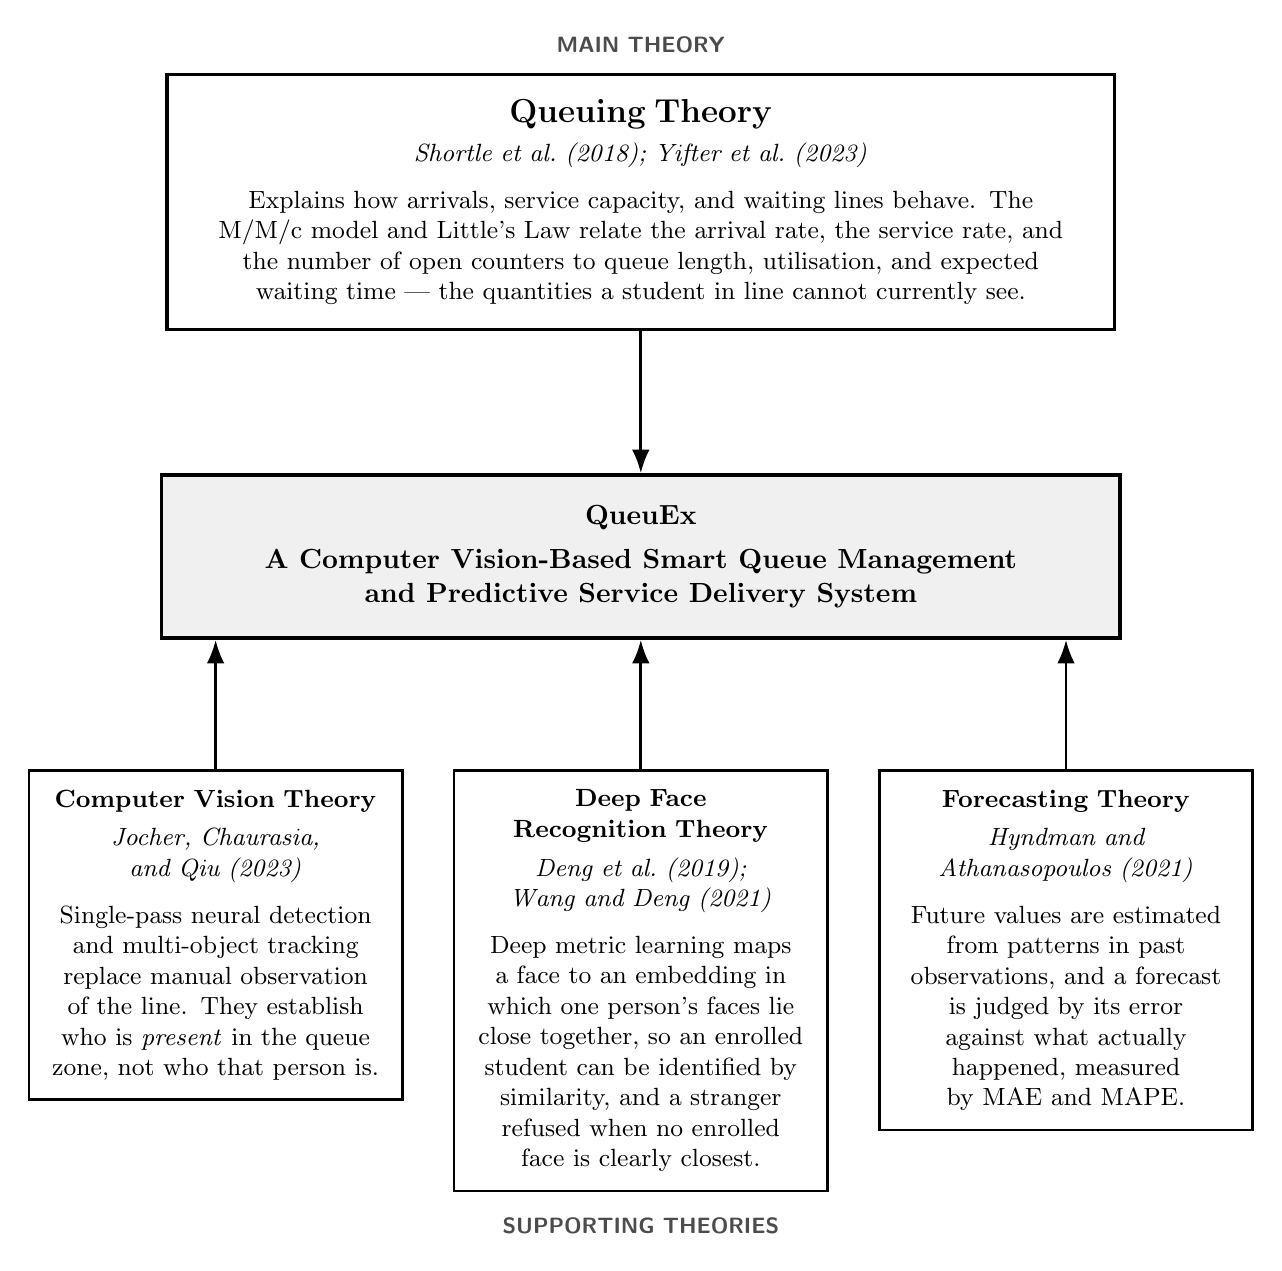
\begin{tikzpicture}[
    every node/.style={align=center},
    tag/.style={font=\footnotesize\bfseries\sffamily, text=black!70},
    mainbox/.style={rectangle, draw=black, line width=1.2pt,
                    text width=11.4cm, inner sep=9pt, font=\small},
    supbox/.style={rectangle, draw=black, line width=0.9pt,
                   text width=4.25cm, inner sep=7pt, font=\small},
    centerbox/.style={rectangle, draw=black, line width=1.4pt,
                      fill=black!6, text width=11.4cm, inner sep=11pt,
                      font=\bfseries},
    arr/.style={-{Latex[length=3mm]}, line width=1pt}
  ]
  \hyphenpenalty=10000
  \exhyphenpenalty=10000
  \node[mainbox] (qt) at (0, 8.2) {
    {\large\textbf{Queuing Theory}}\\[3pt]
    \textit{Shortle et al.\ (2018); Yifter et al.\ (2023)}\\[6pt]
    Explains how arrivals, service capacity, and waiting lines behave.
    The M/M/c model and Little's Law relate the arrival rate, the
    service rate, and the number of open counters to queue length,
    utilisation, and expected waiting time --- the quantities a student
    in line cannot currently see.
  };
  \node[tag, anchor=south] at ([yshift=4pt]qt.north) {MAIN THEORY};

  \node[centerbox] (sys) at (0, 3.7) {
    \sysname{}\\[4pt]
    A Computer Vision-Based Smart Queue Management\\
    and Predictive Service Delivery System
  };

  \node[supbox, anchor=north] (cv) at (-5.4, 1.0) {
    \textbf{Computer Vision Theory}\\[3pt]
    \textit{Jocher, Chaurasia, and Qiu (2023)}\\[6pt]
    Single-pass neural detection and multi-object tracking replace
    manual observation of the line. They establish who is
    \emph{present} in the queue zone, not who that person is.
  };
  \node[supbox, anchor=north] (fr) at (0, 1.0) {
    \textbf{Deep Face Recognition Theory}\\[3pt]
    \textit{Deng et al.\ (2019); Wang and Deng (2021)}\\[6pt]
    Deep metric learning maps a face to an embedding in which one
    person's faces lie close together, so an enrolled student can be
    identified by similarity, and a stranger refused when no enrolled
    face is clearly closest.
  };
  \node[supbox, anchor=north] (ft) at (5.4, 1.0) {
    \textbf{Forecasting Theory}\\[3pt]
    \textit{Hyndman and Athanasopoulos (2021)}\\[6pt]
    Future values are estimated from patterns in past observations,
    and a forecast is judged by its error against what actually
    happened, measured by MAE and MAPE.
  };
  \node[tag, anchor=north] at ([yshift=-6pt]fr.south) {SUPPORTING THEORIES};

  \draw[arr] (qt.south) -- (sys.north);
  \draw[arr] (cv.north) -- (cv.north |- sys.south);
  \draw[arr] (fr.north) -- (sys.south);
  \draw[arr] (ft.north) -- (ft.north |- sys.south);
  \end{tikzpicture}
  \caption{Theoretical Framework of \sysname{}}
  \label{fig:theoretical-framework}
\end{figure}

\emph{Queuing Theory} is the main theory of the study. In its standard
formulation~\cite{shortle2018fundamentals}, and as recent studies of
service queues continue to apply it~\cite{yifter2023modeling}, a waiting
line is described
by the rate at which people arrive, the rate at which a counter serves
them, and the number of counters open. The M/M/c model turns these into
the expected queue length, counter utilisation, and waiting time, and
Little's Law ties the three together: the number of people in a line
equals their arrival rate multiplied by the time each one spends in it.
These are exactly the quantities the baseline survey found students
unable to see --- the highest-scoring student items concerned not knowing
the wait and not knowing how many people are ahead. Queuing theory
therefore defines what \sysname{} must make visible, and it supplies the
wait-time definitions against which the prediction module is judged
under Statement of the Problem No.~3.

\emph{Computer Vision Theory} is the first supporting theory and explains
how the line is observed without a person watching it. Single-stage
detectors of the YOLO family locate every person in a camera frame in
one pass of a neural network, fast enough for continuous
monitoring~\cite{jocher2023}, and multi-object tracking carries each
detection from frame to frame so that a person keeps one identity across
the time they stand in line~\cite{zhang2022bytetrack}. In \sysname{} this
layer answers one question only: whether a person is present in the
queue zone. It does not establish who that person is, and a walk-in who
has not enrolled is detected but never identified.

\emph{Deep Face Recognition Theory} is the second supporting theory and
explains how an enrolled student is recognised. Deep metric learning
trains a network to map each face image to a fixed-length embedding in
which photographs of the same person lie close together and photographs
of different people lie far apart; ArcFace achieves this by adding an
angular margin between identities during training, so that similarity
between two embeddings can be measured by their cosine~\cite{deng2019arcface}.
Recent surveys identify this family of margin-based losses as the basis
of current face recognition~\cite{wang2021deepfacesurvey}.
\sysname{} uses a pretrained model of this kind. The theory explains why
a similarity score is meaningful, but not when a score is high enough to
act on --- particularly in the open-set case, where the person at the
camera may not be enrolled at all. The threshold-and-margin rule that
this study contributes, and evaluates under Statement of the Problem
No.~2, answers that second question.

\emph{Forecasting Theory} is the third supporting theory and explains how
the line is anticipated rather than merely reported. Modern forecasting
practice estimates future values from structure in past observations ---
level, trend, and recurring patterns --- through methods such as
exponential smoothing, and evaluates a forecast by comparing it with what
actually happened~\cite{hyndman2021forecasting}. The same practice names
the error measures used in this study: the Mean Absolute Error, which
states the typical miss in minutes, and the Mean Absolute Percentage
Error, which states it relative to the wait itself. These are the
measures applied under Statement of the Problem No.~3.

Taken together, queuing theory states what the line needs to show,
computer vision establishes who is present in it, face recognition
establishes which of those people are enrolled students entitled to a
system-issued number, and forecasting estimates how long each of them
will wait. The outputs of all four reach users through the staff
dashboard, the student mobile application, and the public display board,
whose usability, reliability, and clarity are assessed under Statement of
the Problem No.~4.


\section{Conceptual Framework}
\label{sec:conceptual-framework}

The conceptual framework follows the Input-Process-Output-Outcome (IPOO)
model. It traces how the camera feed, the students who have enrolled and
asked to be queued, and the staff at the counter are turned by \sysname{}
into a queue that both sides can see.
Figure~\ref{fig:conceptual-framework} arranges the four stages and the
feedback that returns from the outcome to the input.

\begin{figure}[H]
  \centering
  \providecommand{\colbox}[2]{%
    \begin{minipage}[t][8.4cm][t]{#1}\raggedright #2\end{minipage}}
  \begin{tikzpicture}[
    col/.style={rectangle, draw=black, line width=0.9pt, inner sep=4pt,
                anchor=north, font=\footnotesize},
    head/.style={rectangle, fill=black!80, text=white,
                 font=\sffamily\bfseries\small,                  minimum height=0.62cm, anchor=south},
    arr/.style={-{Latex[length=2.8mm]}, line width=1.1pt}
  ]
  \hyphenpenalty=10000
  \exhyphenpenalty=10000

  \node[col] (in) at (0,0) {\colbox{3.0cm}{%
    \textbullet\ Live camera feed of the queue zone\\[4pt]
    \textbullet\ Face embeddings of voluntarily enrolled students\\[4pt]
    \textbullet\ Student's request to be queued (mobile app)\\[4pt]
    \textbullet\ Counter configuration and service times\\[4pt]
    \textbullet\ Staff actions: done, no-show, reset, and emergency manual entry}};
  \node[head, minimum width=3.28cm] at (in.north) {INPUT};

  \node[col] (pr) at (4.23,0) {\colbox{3.9cm}{%
    1.\ Person detection and tracking (YOLOv8n, ByteTrack)\\[4pt]
    2.\ Presence confirmation in the queue zone\\[4pt]
    3.\ Track stability\\[4pt]
    4.\ Face-based identity validation: score $\geq 0.30$ \emph{and}
      margin $\geq 0.15$, else refer to staff\\[4pt]
    5.\ Queue-number issuance for recognised students who asked\\[4pt]
    6.\ Sticky counter assignment\\[4pt]
    7.\ Wait-time prediction\\[4pt]
    8.\ Ticket generation}};
  \node[head, minimum width=4.18cm] at (pr.north) {PROCESS};

  \node[col] (out) at (8.51,0) {\colbox{3.1cm}{%
    \textbullet\ Queue number issued without manual input\\[4pt]
    \textbullet\ Live queue and alerts on the staff dashboard\\[4pt]
    \textbullet\ Position, wait, and a \emph{you're next} prompt in the
      mobile app\\[4pt]
    \textbullet\ Counter calls on the display board, announced by
      voice\\[4pt]
    \textbullet\ Record of every recognition decision}};
  \node[head, minimum width=3.38cm] at (out.north) {OUTPUT};

  \node[col] (oc) at (12.39,0) {\colbox{3.1cm}{%
    \textbullet\ Students know their place and wait without watching the
      display\\[4pt]
    \textbullet\ Hands-free queue entry for registered students\\[4pt]
    \textbullet\ Staff act on the queue earlier\\[4pt]
    \textbullet\ Measured by recognition accuracy (SOP~2), prediction
      error (SOP~3), and satisfaction (SOP~4)}};
  \node[head, minimum width=3.38cm] at (oc.north) {OUTCOME};

  \draw[arr] (in.east)  -- (pr.west);
  \draw[arr] (pr.east)  -- (out.west);
  \draw[arr] (out.east) -- (oc.west);

  % Feedback: from the outcome back to the input, beneath the columns
  \draw[arr, dashed] (oc.south) -- ++(0,-0.75) -| (in.south)
    node[pos=0.25, below, font=\footnotesize\sffamily]
    {FEEDBACK: service times, counter changes, and staff decisions};
  \end{tikzpicture}
  \caption{Conceptual Framework of \sysname{}}
  \label{fig:conceptual-framework}
\end{figure}

\textbf{Input.} The system begins from five inputs. The live camera feed
shows who is standing in the marked queue zone. The face embeddings are
those of students who chose to enrol through the mobile application;
students who have not enrolled contribute no biometric data. A student
who wants a queue number asks for one in the application, so the camera
never queues anyone who did not ask. Walk-ins are not an input to
\sysname{}: they continue to take a ticket from the office's existing
kiosk by pressing its \emph{Get a Ticket} button, a process that runs
separately from this system. The counter
configuration, recent service times, and staff actions at the counter,
including emergency manual entry, complete the inputs.

\textbf{Process.} Eight routines turn these inputs into a managed queue.
The camera pipeline detects and tracks people, confirms which of them are
genuinely standing in the queue zone, and keeps each person's track
stable. For each confirmed person, the face-based identity validation
compares the face against the enrolled roster and accepts a match only
under the two-part threshold-and-margin rule; anyone it cannot identify
with confidence is left for staff rather than guessed at. A recognised
student who has requested a number receives one minted by the system,
and every entry is then given a counter, a wait-time estimate, and a
ticket.

\textbf{Output.} Recognised students receive a queue number without any
manual input. Staff see the live queue, counter assignments, and alerts
for people the system could not identify; students see their own
position, estimated wait, and a prompt when their turn is next; and the
public display board announces counter calls. Every recognition decision
is recorded for later audit.

\textbf{Outcome.} The intended outcome answers the problems found under
Statement of the Problem No.~1: students no longer have to stay within
sight of the display to know where they stand, registered students join
the queue without a manual step, walk-ins are served exactly as before,
and staff can act on the queue earlier. These outcomes are measured by
Statements of the Problem No.~2 to No.~4.

\textbf{Feedback.} Measured service times, changes to the number of open
counters, and staff decisions --- a transaction marked done, a student
marked a no-show, a queue reset --- return to the input stage. They update
the service rate used by the prediction module and the state of the
queue, so that \sysname{} reflects the office as it is operating rather
than the settings it started with.


\section{Statement of the Problem}
\label{cr:sop}

The study is guided by the following research problems:
\begin{enumerate}
  \item What are the current problems with the manual queue management
        process during busy periods, regarding wait times and
        user-experience?
  \item What is the level of accuracy of the face-recognition system
        in identifying enrolled students and assigning queue numbers
        without requiring manual input?
  \item What is the level of accuracy of the system's wait-time
        prediction model in terms of Mean Absolute Error (MAE) and
        Mean Absolute Percentage Error (MAPE)?
  \item What is the level of user's satisfaction in terms of:
        \begin{enumerate}
          \item[(a)] system's usability;
          \item[(b)] system's reliability; and
          \item[(c)] system clarity?
        \end{enumerate}
\end{enumerate}

\section{Assumptions}
\label{cr:assumptions}

The following assumptions delimit the proposed evaluation:

\textbf{Camera visibility and queue-zone coverage.} The camera covers the
queue zone with enough resolution and lighting for YOLO to detect the
people standing in it and for their faces to be detected and recognised
at queue-zone distance, under the lighting and crowd levels typical of
NCF service areas.

\textbf{Stable tracking.} Person tracking keeps each person's identity
stable for as long as they stand in the queue zone, so that their face
can be captured and matched once, and a student who briefly leaves and
returns can be recognised again by face.

\textbf{Student participation.} Students who want a system-issued queue
number have an Android phone and an NCF Gbox account, enrol their face
voluntarily through the mobile application, and ask to be queued before
they reach the queue zone.

\textbf{Representative enrolment.} A student's enrolment photographs
reflect how they look when they queue; a large change in appearance, such
as a face covering not worn at enrolment, may lead the system to refer
them to staff rather than recognise them.

\textbf{Network availability.} The service office has a working internet
connection to the cloud-hosted backend during the evaluation period,
since recognition and queue-number issuance depend on it.

\textbf{Usefulness of prediction outputs.} The implemented prediction
models generate forecasts that are actionable and sufficiently accurate
for staff scheduling and counter management decisions, with accuracy
assessed using MAE and MAPE in Chapter 3.

\textbf{Ticket rendering.} The ticket record remains the same whether
it is printed on thermal paper or rendered as a PDF: both outputs carry
the queue number, short code, QR link, and JWT used for status
checking.

\textbf{Staff capability and system adoption.} Service staff and
administrators possess basic digital literacy to operate the web
dashboard and interpret the system's outputs.

\section{Scope and Delimitation}
\label{sec:scope}

This section describes the boundaries of the \sysname{} study, organized
according to its introduction, scope, and limitations.

\textbf{Introduction.} \sysname{} is a camera-assisted queue management
prototype developed and evaluated for one NCF service-office setting in
Naga City, Philippines. It addresses the specific problem of manual,
observation-based queue handling in a campus service office by combining
automated person detection, face-based identification of enrolled
students, queue-number assignment, ticket generation, and wait-time
prediction in a single prototype system.

\textbf{Scope.} The study covers the development and evaluation of the
\sysname{} prototype in the selected NCF service office. The build
includes the YOLOv8n detection pipeline, self-service face enrolment and
ArcFace-based identification of enrolled students, face-based re-entry
matching, short- and medium-horizon wait-time prediction, FastAPI
endpoints, MySQL storage, a staff dashboard, a student mobile client, and
printer-agnostic ticket generation. During office use, the ticket record
is meant to be printed through a thermal printer. During evaluation, it
is rendered as a PDF so the queue number, short code, QR link, and JWT
validation can be checked without relying on printer availability.

\textbf{Limitations.} The present build uses one camera-defined queue
zone and one selected service office. It excludes multi-zone and
multi-department operation, and no priority queue is implemented in the
system; every queue entry is served in ordinary queue order without
priority handling based on student status or urgency. Face-based
identification and system-issued queue numbers apply only to students
who have enrolled voluntarily and asked to be queued; walk-ins and
unenrolled visitors are detected but never identified, and keep the
printed kiosk number they receive today. The system does not test
whether a face belongs to a live person, so it cannot distinguish a
student from a photograph of that student. The build also excludes
direct links to the Campus Management System or Student Information
System and IoT inputs other than the camera feed and ticket printer.

\sysname{} requires a working internet connection. Its backend,
database, cache, and ticket storage are cloud-hosted, and the detector
in the office must reach the backend for every recognition and every
queue number issued; if the connection fails, recognition and number
issuance stop until it returns. Offline operation is outside the scope
of this build. The user evaluation is limited to a supervised
trial session held before the final defense, not a semester of regular
operation.

\section{Significance of the Study}

The value of the study is in how the prototype supports everyday
service-office work: it gives staff a clearer view of the line,
provides students with a way to check their queue status, and keeps
records that administrators can review when improving service flow.

\textbf{Service Staff.} Service staff receive a dashboard that shows
the active queue, individual wait times, counter assignments, and
short-horizon demand forecasts without requiring them to recount the
line manually.

\textbf{Students.} Students benefit from a queueing process that removes
the counter-side step of asking for a number. A student enrols once, from
their own phone, by signing in with their institutional account and
capturing a face signature. On any later visit they request a place in
the queue in the mobile client and then walk into the monitored area,
where the camera recognizes them and the number is issued without staff
involvement or manual entry. Status is then followed in the mobile client
or through the ticket credential. Because the number is issued only to a
student who has asked for one, recognition alone never places anybody in
the queue.

\textbf{Institutional Administrators.} Administrators receive queue
performance records that can be used when reviewing staffing, service
hours, and physical layout.

\textbf{Naga College Foundation, Inc.} The institution benefits from a
campus-oriented prototype that demonstrates how automation, computer
vision, and predictive analytics can support service delivery and
student-facing operations.

\textbf{Academic Community and Future Researchers.} The work provides a
local reference for combining computer vision, re-identification,
ticket generation, and predictive analytics in Philippine HEI service
queues. Future researchers may extend it to multi-camera zones,
priority queues, direct campus-system integration, or alternative
detection and forecasting models.

\section{Definition of Terms}
\label{cr:definitions}

The following terms are defined operationally as applied in this study.
These definitions clarify the specific meanings of key technical
concepts and system components discussed throughout the manuscript and
are intended to support consistent interpretation of the \sysname{}
prototype and its evaluation.

\textbf{Access Token.} A ticket credential assigned to each confirmed
queue number. In the implemented prototype, this consists of a short
code and a JWT-backed validation record that allows the student to
check queue status without a login account.

\textbf{ArcFace Embedding.} The numeric representation of a face used
throughout this study: a 512-dimensional unit vector produced by the
ArcFace recognition model, in which the cosine similarity between two
vectors expresses how likely they are to belong to the same person. The
transformation runs in one direction only; a face cannot be reconstructed
from its embedding. Embeddings are generated by the InsightFace
\texttt{buffalo\_s} model pack running on the CPU, and the stored
enrolment embedding is the average of those computed from a student's
capture photographs.

\textbf{ByteTrack.} The multi-object tracking
algorithm~\cite{zhang2022bytetrack} invoked by Ultralytics persistent
tracking. ByteTrack associates detection boxes across frames using
high- and low-confidence detection matching, allowing the system to
maintain a stable track identifier $\mathrm{tid}$ for each person as
they move through the queue zone.

\textbf{Candidate Accumulation.} A buffer mechanism requiring a new
detection to appear consistently for a minimum confirmation window of
20 frames, with a centroid-standard-deviation motion check, before a
queue number is assigned. The mechanism prevents shadows, momentary
mis-detections, and stationary mis-classified objects from generating
spurious tickets. The motion gate and confidence bypass are specified
in Section~\ref{subsec:candidate} (\S\ref{subsec:candidate}).

\textbf{Done Cooldown.} A short-lived record of the position a served
person occupied, retained for a fixed number of frames after their
transaction is marked complete. It suppresses an immediate new queue
entry from the same spot, so that a person still standing at the counter
when staff mark them served is not re-admitted to the queue. The record
is spatial and carries no appearance or identity information.

\textbf{Duplicate Suppression.} A per-frame queue-tracker pass that
merges two distinct track identifiers assigned to the same physical
person, retaining the lower queue number. It is guarded by a 60-frame
re-entry immunity counter and an appearance-similarity safeguard that
prevents visually distinct persons from being merged regardless of
geometric proximity. The method is specified in
Section~\ref{subsec:dedup} (\S\ref{subsec:dedup}).

\textbf{Dynamic Service-Time Measurement.} A background process that
recomputes the average transaction service time every five minutes
from inter-departure gaps in the MySQL transaction log, blended
seventy--thirty with the previously stored value. It is specified in
Section~\ref{subsec:service-time} (\S\ref{subsec:service-time}).

\textbf{Exponential Moving Average (Bounding-Box Smoothing).} A
per-frame smoothing pass applied independently to each bounding-box
coordinate using factor $\alpha_{\mathrm{s}} = 0.45$, producing the
visually stable boxes rendered in the staff dashboard's annotated
snapshot.

\textbf{Face Enrolment.} The one-time process by which a student becomes
known to the recognizer. The student signs in with their institutional
account and then submits one to five photographs from the mobile client,
from which a single averaged ArcFace embedding is computed and stored
against their profile. The photographs are discarded once the embedding
is derived and are never written to storage. A student may repeat the
process, which replaces the stored embedding.

\textbf{Holt's Double Exponential Smoothing.} A classical forecasting
algorithm~\cite{holt2004forecasting} used for the medium-horizon
prediction, applying separate smoothing parameters for queue level and
trend, together with a damping factor to avoid over-projection.
Parameter values used in the prototype are configurable defaults
reported and justified in Chapters 2 and 3.

\textbf{Join Intent.} The student's explicit request, made in the mobile
client before approaching the service office, to be issued a queue number
when the camera recognizes them. It is the consent gate that separates
recognition from enrolment in the queue: a registered student who is
recognized without having armed a join intent is classified as a
bystander and issued nothing. The intent lapses after a configurable
interval and is consumed once it produces a number, so each visit
requires a fresh request.

\textbf{M/M/c Model.} A foundational multi-server queueing model from
classical queueing theory~\cite{shortle2018fundamentals} used for
short-term wait-time prediction, calculating $W = L/\lambda$ from
Little's Law using real-time arrival rates from the YOLO detection
pipeline.

\textbf{Mobile Client.} The student-facing application through which a
student signs in with an NCF Gbox account, enrols a face voluntarily,
asks to be queued, and follows their own position and estimated wait.
It is implemented as a Flutter application for Android and communicates
with the backend through the student API; references to the ``mobile
application'' elsewhere refer to the same component.

\textbf{Non-Maximum Suppression (NMS).} A standard
intersection-over-union pass applied internally by ByteTrack during
detection to suppress overlapping bounding-box candidates. A separate
per-frame duplicate-suppression step at the queue-tracker level,
specified in Section~\ref{subsec:dedup} (\S\ref{subsec:dedup}), handles the related
but distinct case of two track identifiers being assigned to the same
physical person within the same frame.

\textbf{Open-Set Rejection.} The requirement that the recognizer refuse
any face it has not enrolled, rather than returning the closest match
available. A closed-set recognizer always names somebody; an open-set one
must be able to answer that the person is unknown. In \sysname{} this is
enforced by the threshold-and-margin decision rule, and it is what allows
unenrolled visitors to pass through the queue zone without ever being
identified.

\textbf{Printer-Agnostic Ticket Protocol.} The set of fields, including
queue number, short code, QR link, and JWT, issued for each confirmed queue
entry. Because the ticket record is independent of the output device,
it can be printed on thermal paper in office use or rendered as a PDF
during evaluation.

\textbf{Public Display Board.} A user-facing surface, alongside the
staff web dashboard and the student mobile client, that renders the
active queue in the waiting area and announces newly assigned counter
calls using the browser's built-in Web Speech API. All
text-to-speech synthesis runs client-side; no audio is transmitted to
any external service.

\textbf{Queue Zone.} A configurable rectangular region defined by four
pixel coordinates on the camera frame; only persons whose bounding box
centre falls within this region are tracked and assigned queue numbers.

\textbf{Re-Entry Matching.} The procedure that restores a queue person
whose track was lost, typically because they stepped out of the camera's
view and returned. A face embedding taken from the new detection is
compared against the stored embeddings of queue persons currently
recorded as missing, and the same threshold-and-margin decision rule used
elsewhere in the system governs acceptance. A face signature is
discriminative enough on its own that the earlier tiered scheme of
recency windows, spatial fallbacks and lookalike safeguards, which
existed to compensate for weak clothing-colour comparison, is no longer
required.

\textbf{Sticky Counter Assignment.} A scheduling rule under which a
counter, once allocated to a queue entry, persists until that entry is
marked done or a no-show, regardless of changes to the line behind it.
The rule prevents the disorienting per-frame reshuffling that a
straight-rank assignment would otherwise produce.

\textbf{Threshold-and-Margin Decision Rule.} The two-part test every face
match must pass before it is accepted. The cosine similarity to the
best-matching enrolled student must reach an absolute threshold
$\tau_{\mathrm{match}} = 0.30$, and it must additionally exceed the
similarity to the second-best candidate by a margin
$\tau_{\mathrm{margin}} = 0.15$. The first condition establishes that the
face resembles a known student at all; the second establishes that it
resembles one student distinctly more than any other. A match that
satisfies the threshold but not the margin is refused rather than
resolved by choosing the higher score, so an ambiguous face produces no
identification instead of a plausible but unverified one.

\textbf{You Only Look Once (YOLO).} The YOLOv8n
model~\cite{jocher2023} with ByteTrack-based \texttt{persist=True}
tracking, configurable input size, and confidence threshold, used to
detect and track persons entering the queue zone in camera frames. Newer
variants, YOLOv9 through YOLOv12~\cite{tian2025yolov12}, are not used
in this study; the rationale is discussed in Section~1.3.

% ============================================================
% CHAPTER 2: METHODOLOGY
% ============================================================
\chapter{Methodology}

Chapter~2 sets out how the \sysname{} prototype will be built, deployed,
and evaluated in the selected NCF service office. The chapter covers
the research design, respondents and locale, sampling procedure, data
gathering, research instruments, questionnaire validation, ethical
safeguards, statistical treatment, system architecture, development
process, and testing plan.

\section{Research Design}

The research design has two linked parts. The developmental part covers
the construction of \sysname{}; the evaluation part checks how the
prototype behaves during service-office use. Quantitative evidence
comes from system logs, observer records, and survey ratings. These
data are used to measure queue assignment accuracy, re-identification
reliability, ticket and token validation, detection-to-ticket latency,
and wait-time prediction error through Mean Absolute Error (MAE) and
Mean Absolute Percentage Error (MAPE). The five-point Likert survey
records how cashier staff and student users rate
dashboard usability, layout clarity, and the usefulness of the
prediction outputs after regular exposure to the prototype.
Qualitative evidence comes from short semi-structured interviews, where
respondents can explain concerns or useful features that a rating scale
may not capture.

The engineering work is organized around the prototype components that
carry the main technical risk: YOLOv8n detection, hybrid re-entry
matching, ticket-payload generation, multi-horizon prediction, the
FastAPI backend, the staff dashboard, and the mobile status interface.
Each component is built through the Agile sprint cycle described in
Section~\ref{sec:sdp}.
Its output is checked against the design principles in
Section~\ref{sec:design-arch}. Quantitative results and qualitative
accounts are analyzed side by side so that the final discussion can
compare measured performance with the actual experience of the users.

\section{Population and Locale of the Study}
\label{cr:population}

Naga College Foundation, Inc.\ (NCF), located in Naga City, Camarines
Sur, Philippines, serves as the locale of this study. NCF was selected
as the research site because its service offices, particularly the
cashiering office, experience high student traffic during enrollment,
payment, and clearance periods, creating visible peak-demand conditions
that are appropriate for evaluating a camera-assisted queue management
prototype. The prototype will be installed in one service office area
coordinated with NCF administration, serving as the single-queue-zone
test site defined in the Scope and Delimitation of Chapter~1.

The study population consists of the two groups who directly use the
\sysname{} prototype. The first is the cashier staff assigned to the
selected cashiering office counter, who operate the staff dashboard. The
second is currently enrolled NCF students who transact at the cashiering
office and receive a \sysname{}-issued queue number. Administrators and
IT personnel are not surveyed: they oversee the office but do not use the
system themselves, so they could not rate its usability, reliability, or
clarity from experience. The total population size for each
group will be determined prior to deployment in coordination with NCF
administration, and the number of respondents drawn from each group is
reported in the final evaluation phase of Chapter~3.

\section{Sample and Sampling Technique}
\label{cr:sampling}

This study uses total enumeration for cashier staff and convenience
sampling for students, adapted to the supervised trial session in which
the system is evaluated. Sampling is adapted to the size and role of
each group rather than applying one procedure to both, so that the
evaluation includes the operational perspective of staff and the user
experience of students.

\textbf{Service staff.} Because the population of staff directly
involved in queue-based transactions in the selected service office is
relatively small and bounded, total enumeration is used; all eligible
staff will be invited to participate. The inclusion criterion is
having operated the staff dashboard during the supervised trial
session.

\textbf{Students.} Student respondents are drawn by convenience
sampling from the students who volunteer for the supervised trial
session. Each goes through the full sequence: signing in, enrolling a
face, asking to be queued, and being issued a queue number at the queue
zone. The inclusion criterion is completing that sequence at least once
during the session. This replaces the Slovin-sized sample stratified by
year level in the original design, as explained in
Section~\ref{sec:datagathering}; the student sample is therefore smaller
and is not claimed to represent all NCF students.

\textbf{Baseline respondents.} The baseline survey for Statement of the
Problem No.~1 is a separate, earlier sample drawn by convenience
sampling. A link to the online questionnaire was shared with students
and service staff of NCF, and those who chose to answer formed the
sample: 22 in all, 15 students and 7 staff members. Because respondents
selected themselves, the sample may over-represent people with stronger
views about the queue, and it was not sized by Slovin's formula; it is
also small, particularly on the staff side. Its results are therefore
read as evidence of what the current problems are and how strongly each
group feels them, not as estimates for the whole NCF population.

\textbf{Exclusion criterion.} In both groups, any prospective
respondent below 18 years of age is excluded. The age criterion is
enforced through a screening question that immediately precedes the
informed consent form, and any prospective respondent indicating an age
below 18 is thanked for their interest and not enrolled.

\section{Data Gathering Procedure}
\label{sec:datagathering}

Data gathering is divided into three phases so that the manual
baseline, live system behavior, and user feedback are not mixed
together prematurely. The sequence also makes it possible to compare
what staff normally do, what \sysname{} records during use, and what
participants report after using the prototype.

\textbf{Phase 1: Pre-Deployment Setup and Operational Baseline.} Prior
to deployment, the researchers will coordinate with the office head of
the selected service office to confirm the camera placement, queue zone
calibration, counter configuration, and the initial seed value for the
average service time. The seed value is used by the prediction service
until enough transactions have been logged for the dynamic
service-time measurement procedure (Section~\ref{subsec:service-time},
\S\ref{subsec:service-time}) to supply a measured estimate. During this phase, the
researchers will also conduct informal observation of the existing
manual queue handling process, recording approximate queue lengths and
qualitative accounts from staff regarding the patterns of congestion
most commonly encountered. The baseline questionnaire described in
Section~\ref{sec:instrument} was administered online through a shared
questionnaire link from 16 to 23 September 2026, and its results
answer Statement of the Problem No.~1. These baseline accounts establish
the reference against which the \sysname{}-mediated process is later
compared.

\textbf{Phase 2: System Deployment and Performance Logging.} After
alpha testing in Section~2.10, the system will be operated in the
selected service office during the supervised trial session. During this phase, two parallel streams of data will be
captured. First, the system will automatically log every detection
event, queue assignment, re-entry matching decision, ticket issuance,
prediction output, and dashboard interaction, with associated
timestamps. Second, an independent observer will maintain a manual
ground-truth log during defined observation windows, recording each
actual queue entrant, each genuine re-entry event, and the actual wait
time measured from queue zone entry to counter arrival. The automated
logs and the manual ground-truth log together support the technical
performance metrics specified in Section~2.7.

\textbf{Phase 3: Post-Trial Survey and Interviews.} Immediately after
the supervised trial session, the content-validated questionnaire in
Section~2.5 will be administered to the respondent groups identified in
Section~2.3.
A subset of respondents from each group will be invited to a short
semi-structured interview, scheduled at their convenience and lasting
approximately twenty minutes. Interview audio will be recorded only
with consent and transcribed, after which the recordings will be
deleted. Both survey responses and interview transcripts will be
anonymized before analysis.

\textbf{Shortened evaluation protocol.} The original design allowed at
least two weeks of regular operation before the user evaluation, a
separate pilot of 10 to 15 respondents before the main survey, and a
student sample sized by Slovin's formula. The time available before the
final defense does not allow these, so the protocol was shortened in
three ways, each reported here rather than left implicit. First, the two
weeks of regular operation are replaced by a single supervised trial
session, and the questionnaire is answered immediately afterwards.
Second, the separate pilot is replaced by Cronbach's alpha computed on
the evaluation responses themselves. Third, the student sample consists
of the volunteers who complete the trial rather than a Slovin-sized
sample. Content validation by the three expert raters is kept. The
consequence for interpretation is direct: the results for Statement of
the Problem No.~4 describe users' first experience of \sysname{} under
supervision, not their satisfaction after sustained daily use, and they
are reported with that qualification.

\section{Research Instrument}
\label{sec:instrument}

Four instruments provide the evidence for the study: the \sysname{}
operational log, the observer's ground-truth log, a researcher-made
Likert questionnaire, and a short semi-structured interview guide.

\textbf{Operational and ground-truth logs.} The operational log is
generated automatically by the system and records every detection,
queue assignment, re-entry decision, ticket issuance, prediction
output, dashboard action, and associated timestamps. The manual
ground-truth log is a paper or digital record maintained by an
independent observer during defined observation windows in Phase~2.
Together these two logs provide the data needed to compute queue
assignment accuracy, re-identification reliability, MAE and MAPE for
wait-time prediction, detection-to-ticket latency, and ticket and token
validation rates.

\textbf{Baseline questionnaire.} A separate researcher-made
questionnaire addresses Statement of the Problem No.~1 and is
administered before deployment. It exists in two forms against a shared
five-point scale, because the two groups experience the queue from
opposite sides: the staff form asks about running the queue, and the
student form about waiting in it. Each form contains fourteen items in
two sections --- seven on perceived problems with wait-time and seven
on perceived problems with user experience --- followed by one
open-ended question asking, in the respondent's own words, what the
biggest problem is. Every item is worded as a problem, so agreement
indicates that the problem is present; only the agreement half of
Table~\ref{tab:likert} is therefore applied to this instrument, since
its quality half inverts the meaning of a problem statement. Its
internal consistency is tested with Cronbach's alpha for each section
and for each form as a whole, and the coefficients are reported with the
results in Chapter~3. The staff form also records tenure and how often the respondent handles the
queue; the student form records year level and frequency of use. The
full instrument appears in Appendix~\ref{app:sop1-questionnaire}.

\textbf{Likert-scale questionnaire.} A second questionnaire is
structured into three dimensions that correspond directly to Statement
of the Problem No.~4 in Chapter~1: (a)~system's usability, covering the
dashboard, mobile client, and ticket workflow; (b)~system's
reliability, covering queue assignment accuracy, face recognition,
and re-identification as perceived by users; and (c)~system clarity,
covering the dashboard layout, live snapshot, analytics cards, counter
controls, and the presentation of wait-time predictions. Each respondent
answers fifteen items, five per dimension: two common to all groups, so
that the groups can be compared, and three specific to their role. The
items are rated on the five-point scale shown in Table~\ref{tab:likert}
and listed in Appendix~\ref{app:queueflow-questionnaire}.

\textbf{Semi-structured interview guide.} A short interview guide is
prepared to explore usability problems, perceived benefits of the
prediction outputs, situations in which staff would override system
suggestions, and recommendations for future improvement. The guide is
used flexibly, with the interviewer free to follow up on respondent
comments.

\begin{table}[!ht]
  \caption{Likert Scale Interpretation}
  \label{tab:likert}
  \centering
  \begin{tabular}{clcc}
    \toprule
    \textbf{Scale} & \textbf{Category} & \textbf{WM Range} &
    \textbf{Interpretation} \\
    \midrule
    5 & Strongly Agree    & 4.21--5.00 & Strongly Agree / Excellent \\
    4 & Agree             & 3.41--4.20 & Agree / Very Satisfactory \\
    3 & Neutral           & 2.61--3.40 & Neutral / Satisfactory \\
    2 & Disagree          & 1.81--2.60 & Disagree / Poor \\
    1 & Strongly Disagree & 1.00--1.80 & Strongly Disagree / Very Poor \\
    \bottomrule
  \end{tabular}
\end{table}

\textbf{Instrument validation.} Because the questionnaire is
researcher-made, its content validity is established before it is
used, and its reliability is measured on the responses. Content validation is
conducted by three expert raters, namely the thesis adviser, one
faculty member with expertise in research methods or statistics, and
one faculty member with expertise in computer science or information
systems. Each rater independently rates every item on a four-point
relevance scale, where 1 means not relevant and 4 means highly
relevant. The Content Validity Index is then computed at the item level
(I-CVI) and at the scale level (S-CVI/Average). An I-CVI of at least
0.78 per item and an S-CVI/Average of at least 0.90 for the full scale
are taken as acceptable thresholds, and any item falling below the
threshold is revised or removed based on the experts' written comments.
Under the shortened evaluation protocol this is completed in a single
review round before the questionnaire is administered.

\textbf{Reliability testing.} Internal-consistency reliability is
computed with Cronbach's alpha, using the formula in Section~2.7, for
each dimension within each respondent group, and a value of at least
0.70 is taken as acceptable. The original design called for a separate
pilot of 10 to 15 respondents excluded from the final sample; under the
shortened evaluation protocol, alpha is instead computed on the
evaluation responses themselves, as it was for the baseline
questionnaire. A dimension that falls below 0.70 is reported with its
coefficient and interpreted item by item rather than as a composite. The
signed content validation forms and the reliability output are attached
as appendices.

\section{Ethical Considerations}
\label{sec:ethics}

Ethical handling is treated as part of the system design, not only as a
research requirement. Staff and student users may join
surveys, interviews, and system testing only after giving informed
consent. Before any questionnaire or interview is administered, the
researchers explain the purpose of the study, the activities involved,
the expected time commitment, possible benefits, and the participant's
right to withdraw without penalty.

Only respondents who are 18 years of age or older will be enrolled. The
age criterion is enforced through a screening question that immediately
precedes the consent form, and any prospective respondent indicating an
age below 18 will not be enrolled. No data from minors is collected or
stored at any point in the study.

For confidentiality, personal identifiers are removed before analysis.
Questionnaires use respondent codes instead of names. Interview audio,
when the respondent allows recording, is transcribed for analysis and
then deleted. Results are reported in aggregate form so that individual
respondents are not identifiable. Digital files are kept in
password-protected storage accessible only to the researchers and the
thesis adviser, while hard-copy materials are placed in locked storage
and shredded after the retention period. Study data are kept for a
maximum of three years after completion and are then destroyed.

\textbf{Camera Snapshot Handling.} The system captures live video
frames from the queue zone solely for automated person detection and
the live staff dashboard. The detector encodes annotated snapshots,
showing the camera frame with queue zone, person bounding boxes, and
queue numbers overlaid, at a configurable frame rate and transmits them
to the backend through an authenticated endpoint. The backend retains
only the latest snapshot in process memory; each new snapshot
overwrites the previous one, and no historical snapshot archive is
maintained on disk. Where an optional Redis cache is enabled in cloud
deployment, it is configured as a volatile cache only: snapshot keys
carry a short time-to-live, with a default of ten seconds, and Redis
persistence, including RDB snapshotting and AOF append-only logging, is
disabled in the bundled Redis configuration
(\texttt{save ""; appendonly no}). If a managed Redis provider is used,
persistence and provider-side backups for the \sysname{} cache instance
must be disabled, or the existence of provider-side persistence must be
disclosed in the deployment notes. Detection metadata, including person
tracks, queue length, and wait-time predictions, is transmitted through
a separate endpoint and is the only data persisted in the MySQL
database; the snapshot image itself is not written to MySQL at any
point. The queue-zone camera does perform face recognition on enrolled
students, and the handling of that biometric data is set out separately
below.

\textbf{Biometric Data and Face Enrolment.} Following the panel-mandated
revision, \sysname{} identifies enrolled students by face rather than by
clothing appearance. This constitutes processing of sensitive personal
information under Section~3(l) of the Data Privacy Act of 2012, and it is
treated as such.

Enrolment is self-service and requires two deliberate acts. A student
signs in with an institutional Gbox account and then completes a separate
face-capture step; neither alone enrols anyone. The capture submits one to
five photographs taken at varied angle and lighting, from which the system
computes a single averaged 512-dimensional ArcFace embedding. The
photographs themselves are never written to storage: they are read into
memory, converted to the embedding, and discarded within the same request.
No table in the database holds a face image, and the embedding is a
one-way numeric representation from which the original face cannot be
reconstructed.

That embedding, held in \texttt{student\_profiles}, is the only biometric
artefact the system retains. Embeddings computed at the queue-zone camera
during operation exist in process memory for the lifetime of a person's
track and are never written to the database; the recognition audit table
records only the matched student identifier, the similarity score, the
margin over the runner-up, and the accept-or-reject outcome.

Recognition is not treated as consent to be queued. A recognized student
is issued a number only if they have separately requested one in the
mobile client, and that request lapses after a configurable interval. A
registered student who merely walks past the camera is marked as a
bystander and is issued nothing. People who are not enrolled are never
identified: acceptance requires both an absolute similarity threshold and
a margin over the next-best candidate, and the matcher refuses rather than
guesses when either condition fails.

Withdrawal is supported. A hard-delete path removes a student profile
together with its embedding in support of erasure requests under the Act,
and a student may re-enrol at any time, which replaces the stored
embedding rather than adding to it.

\textbf{Access Control and Transparency.} Dashboard access is
restricted to authenticated staff through session login, with JWT-based
camera-token validation between the detector and the backend. The
student-facing mobile client exposes only the requesting student's own
queue status, reached either through the signed-in student's own session
or through the ticket QR code and short-code credential issued to that
student; it does not display the camera feed or any other student's
status. Physical signage will be posted at the
service-office entrance informing visitors that the area is monitored
by an automated queue management system for service-delivery purposes,
that students who have enrolled a face signature are identified by the
camera while all other persons are detected but never identified, and
that enrolment is voluntary and may be withdrawn. The signage cites the
Data Privacy Act of 2012, or Republic Act No.~10173, and provides
researcher contact for data-subject requests. The camera is
mounted visibly, not concealed. Consistent with the proportionality
principle of the Act, only the minimum data necessary for queue
management is processed; no marketing, profiling, or third-party data
sharing is performed.

The work is aligned with the Data Privacy Act of 2012, or Republic Act
No.~10173, and with applicable NCF research ethics protocols. Ethical
clearance will be secured from the host institution before deployment
and data collection begin. Sources are cited and acknowledged
throughout the manuscript. Any use of AI-assisted tools is limited to
draft organization, language checking, or proofreading; the system
implementation, analysis, interpretation, and final responsibility for
the manuscript remain with the researchers.

\section{Statistical Treatment of Data}

The statistical treatment is organized around the questions raised in
Chapter~1. Technical measures are used for the detector, ticket, and
prediction components, while descriptive statistics are used for the
respondent ratings and profile data.

\textbf{Queue Assignment Accuracy and Re-Identification Reliability.}
These two metrics address Statement of the Problem No.~2. Queue
assignment accuracy is computed as the proportion of correctly assigned
queue numbers, matching the manual ground-truth log, over the total
number of arrivals observed during the evaluation period.
Re-identification reliability is computed as the proportion of correct
re-entry decisions, either correctly restoring a previous queue number
or correctly assigning a new one, over the total number of re-entry
events observed:
\begin{equation}
  \text{Accuracy} =
  \frac{\text{correct decisions}}{\text{total decisions}} \times 100\%
  \label{eq:accuracy}
\end{equation}

\textbf{Face-Recognition Accuracy.} Recognition is additionally
evaluated offline on photographs whose identities are known, so that its
accuracy can be measured against ground truth rather than inferred from
the system's own log. Each held-out probe is compared with every
enrolled identity. A comparison between a probe and its own identity is
a \emph{genuine} pair; any other comparison is an \emph{impostor} pair.
At a match threshold $\tau$, the False Accept Rate is the proportion of
impostor pairs that score at or above $\tau$, and the False Reject Rate
is the proportion of genuine pairs that score below it:
\begin{equation}
  \text{FAR}(\tau) =
  \frac{\left|\{\text{impostor pairs with } s \geq \tau\}\right|}
       {\left|\{\text{impostor pairs}\}\right|}, \qquad
  \text{FRR}(\tau) =
  \frac{\left|\{\text{genuine pairs with } s < \tau\}\right|}
       {\left|\{\text{genuine pairs}\}\right|}
  \label{eq:far-frr}
\end{equation}
The Equal Error Rate (EER) is the value at which the two rates coincide,
and the area under the ROC curve (AUC) is the probability that a
randomly chosen genuine pair outscores a randomly chosen impostor pair;
both describe the embedding model independently of any threshold. The
decision rule itself is then evaluated at the deployed thresholds as an
identification outcome for each probe --- correctly linked, linked to
the wrong identity, or refused and escalated to staff --- and, in an
open-set test, by removing each person from the gallery and probing
with their photographs, so that the rate at which a non-enrolled person
is wrongly identified can be measured directly.

\textbf{Mean Absolute Error and Mean Absolute Percentage Error.} These
two metrics address Statement of the Problem No.~3 and are computed
separately for the current, 5-minute, 15-minute, and 30-minute
prediction horizons:
\begin{equation}
  \text{MAE} =
  \frac{1}{n}\sum |y_{\text{predicted}} - y_{\text{actual}}|
  \label{eq:mae}
\end{equation}
\begin{equation}
  \text{MAPE} = \frac{1}{n}\sum\left|
    \frac{y_{\text{actual}} - y_{\text{predicted}}}{y_{\text{actual}}}
  \right| \times 100\%
  \label{eq:mape}
\end{equation}
where $y_{\text{predicted}}$ is the system's wait-time estimate at a
given horizon and $y_{\text{actual}}$ is the wait time measured by the
observer using a stopwatch from queue zone entry to counter arrival.

\textbf{Weighted Mean and Overall Weighted Mean.} These two measures
address Statements of the Problem No.~1 and No.~4. For No.~1 they are
computed separately for staff and students, whose baseline items
differ, and are interpreted on the agreement scale only. The weighted
mean (WM) is
computed for each Likert item, each dimension averaged across items
within a dimension, and each respondent group: cashier staff and
students. The results are then pooled into an
overall weighted mean (OWM). Per-group weighted means are reported to
allow comparison across stakeholder perspectives; because staff and
students answer different role-specific items for No.~4, groups are
compared on the common items only.
\begin{equation}
  \text{WM} = \frac{\sum(f \times w)}{N}
  \label{eq:weighted_mean}
\end{equation}
where $f$ is the frequency of each response, $w$ is the weight assigned
to that response from 1 to 5 on the Likert scale, and $N$ is the number
of respondents in the group.
\begin{equation}
  \text{OWM} = \frac{\sum \text{WM}}{n}
  \label{eq:overall_weighted_mean}
\end{equation}
where $n$ is the number of items per dimension or the number of
dimensions per group, depending on which level of aggregation is being
computed. Interpretation follows the verbal categories in
Table~\ref{tab:likert}.

\textbf{Percentage Distribution.} Percentage is used to describe the
composition of the respondent sample by group, year level, role, and
demographic profile, and the distribution of responses across the
five-point scale for each item:
\begin{equation}
  P = \frac{f}{N} \times 100
  \label{eq:percentage}
\end{equation}

\textbf{Cronbach's Alpha.} Cronbach's alpha is used to assess the
internal-consistency reliability of the questionnaire after the pilot
test:
\begin{equation}
  \alpha =
  \frac{k}{k - 1}
  \left(1 - \frac{\sum\sigma_i^2}{\sigma_{\text{total}}^2}\right)
  \label{eq:cronbach_alpha}
\end{equation}
where $k$ is the number of items, $\sigma_i^2$ is the variance of each
item, and $\sigma_{\text{total}}^2$ is the variance of the total score.
Values of 0.70 or higher are taken as acceptable.

\textbf{Detection-to-Ticket Latency.} Detection-to-ticket latency is
reported as the mean and standard deviation, in seconds, of the elapsed
time from the first confirmed detection of a queue entrant to the
issuance of the corresponding ticket payload, computed from the
automated operational log.

\section{System Design and Architecture}
\label{sec:design-arch}

\sysname{} is designed as a set of cooperating components rather than as
a single monolithic application. The detector, re-identification logic,
ticket workflow, prediction module, dashboard, FastAPI backend, and
MySQL data layer are developed and tested iteratively so that changes
in one component can be checked against the behavior of the rest of the
prototype.

\subsection{Design Principles}

\textbf{Recognition Accuracy.} The system must never issue an enrolled
student's queue number to someone else. Person detection establishes
only that someone is present; a queue number is issued only when the
face-based identity validation accepts an enrolled student under the
threshold-and-margin rule, and anyone the rule cannot identify with
confidence is referred to staff rather than guessed at. Recognition
accuracy, the rate of wrong identities, and the rejection of
non-enrolled people are the primary quality gates, reported in
Chapter~3.

\textbf{Prediction Usefulness.} The prediction module must produce
wait-time estimates whose MAE and MAPE, at each of the current,
5-minute, 15-minute, and 30-minute horizons, are low enough to be
actionable for staff planning. Specific target thresholds are reported
in Chapter~3.

\textbf{API Reliability.} The REST endpoints must handle malformed,
empty, or unusually long inputs gracefully, returning structured error
responses rather than crashing. Endpoint behavior must be consistent
and deterministic across repeated calls with identical inputs, and
inference time must remain within bounded latency for live use.

\textbf{Reproducibility.} All model configurations, queue-zone
parameters, prediction smoothing factors, and confirmation-window
values used in the prototype are recorded as configurable defaults in
version-controlled code stored in the project repository, ensuring
results reported in this study can be independently verified.

\textbf{Privacy Protection.} Consistent with the visual privacy
literature reviewed in Chapter~1, the system stores derived data rather
than imagery. Detection produces bounding boxes, and identification
produces face embeddings, which are one-way numeric representations from
which a face cannot be reconstructed. No photograph, video segment or
camera frame is written to the database at any point, and enrolment
photographs are discarded once their embedding has been computed. Because
the embedding is nonetheless biometric data, its handling is governed by
the safeguards set out in Section~\ref{sec:ethics}.

\subsection{Tools and Technologies}

\sysname{} is split between the service office and the cloud. The
detector runs on the camera-connected machine in the office, where it
performs person detection and computes face embeddings locally, so that
no camera frame has to leave the building for recognition. The backend,
database, cache, and ticket storage are hosted in the cloud, and the
staff dashboard and student mobile application reach them over the
internet. Table~\ref{tab:tools} lists the tools used in each part and
the reason each was chosen.

\begin{table}[!htbp]
  \caption{System Tools and Technologies}
  \label{tab:tools}
  \centering
  \footnotesize
  \renewcommand{\arraystretch}{1.05}
  \begin{tabular}{p{2.3cm} p{3.4cm} p{7.4cm}}
    \toprule
    \textbf{Category} & \textbf{Technology} & \textbf{Rationale} \\
    \midrule
    Person detection & YOLOv8n (Ultralytics) with ByteTrack &
      Lightweight single-pass person detection with persistent tracking,
      fast enough to run on an office computer without a dedicated
      GPU~\cite{jocher2023,zhang2022bytetrack}. \\
    Face recognition & InsightFace \texttt{buffalo\_s} on ONNX Runtime (CPU) &
      Pretrained face detector and ArcFace embedding
      network~\cite{deng2019arcface}; the smallest general-purpose pack,
      chosen to fit the 512~MB backend limit. \\
    Video & OpenCV &
      Camera capture, frame preprocessing, overlays, and JPEG encoding of
      the live view. \\
    Backend API & Python, FastAPI, Uvicorn &
      REST endpoints for the detector, the staff dashboard, and the
      student application; live MJPEG stream of the queue camera. \\
    Staff dashboard & React, TypeScript, Vite, Tailwind CSS &
      Browser-based dashboard for the live queue, counter control,
      Done and No-show actions, pending-link alerts, and analytics. \\
    Student application & Flutter (Android) &
      Sign-in, face enrolment, joining the queue, and viewing position
      and estimated wait. \\
    Student sign-in & Google Sign-In (NCF Gbox) &
      Restricts accounts to the school's own domain, so no separate
      password system is needed. \\
    Database & MySQL (managed, Aiven) &
      Student profiles and face embeddings, queue records, tickets,
      events, and the recognition audit. \\
    Cache & Redis (managed, Upstash) &
      Short-lived shared state for the live queue; keys expire and are
      not persisted. \\
    Ticket storage & S3-compatible object storage (Supabase) &
      PDF tickets, kept outside the backend container so they survive a
      restart. \\
    Hosting & Render (Docker), Vercel &
      Backend container on Render; staff dashboard on Vercel. \\
    Ticketing & Short code, JWT (HS256), QR code &
      Ticket credential for status checking; PDF during evaluation and
      thermal printing in deployment. \\
    Prediction & Custom Python &
      M/M/c baseline, trend projection, and exponential smoothing for the
      wait-time estimates. \\
    Development & VS Code, Git/GitHub, Postman, Docker &
      Version control, endpoint testing, and reproducible builds. \\
    \bottomrule
  \end{tabular}
\end{table}


\subsection{System Architecture}
\label{sec:architecture}

\sysname{} follows a six-layer architecture: the Presentation Layer, the
API Layer, the Computer Vision Layer, the Business Logic Layer, the
Persistence Layer, and the Cache and Runtime State Layer. The layers also
divide by location. The Computer Vision Layer runs on the office computer
attached to the camera; every other layer runs in the cloud, and the
dashboard and mobile application reach it over the internet.
Figure~\ref{fig:system-architecture} shows the layers and their
components.

\begin{figure}[!htbp]
  \centering
  \resizebox{\textwidth}{!}{%
  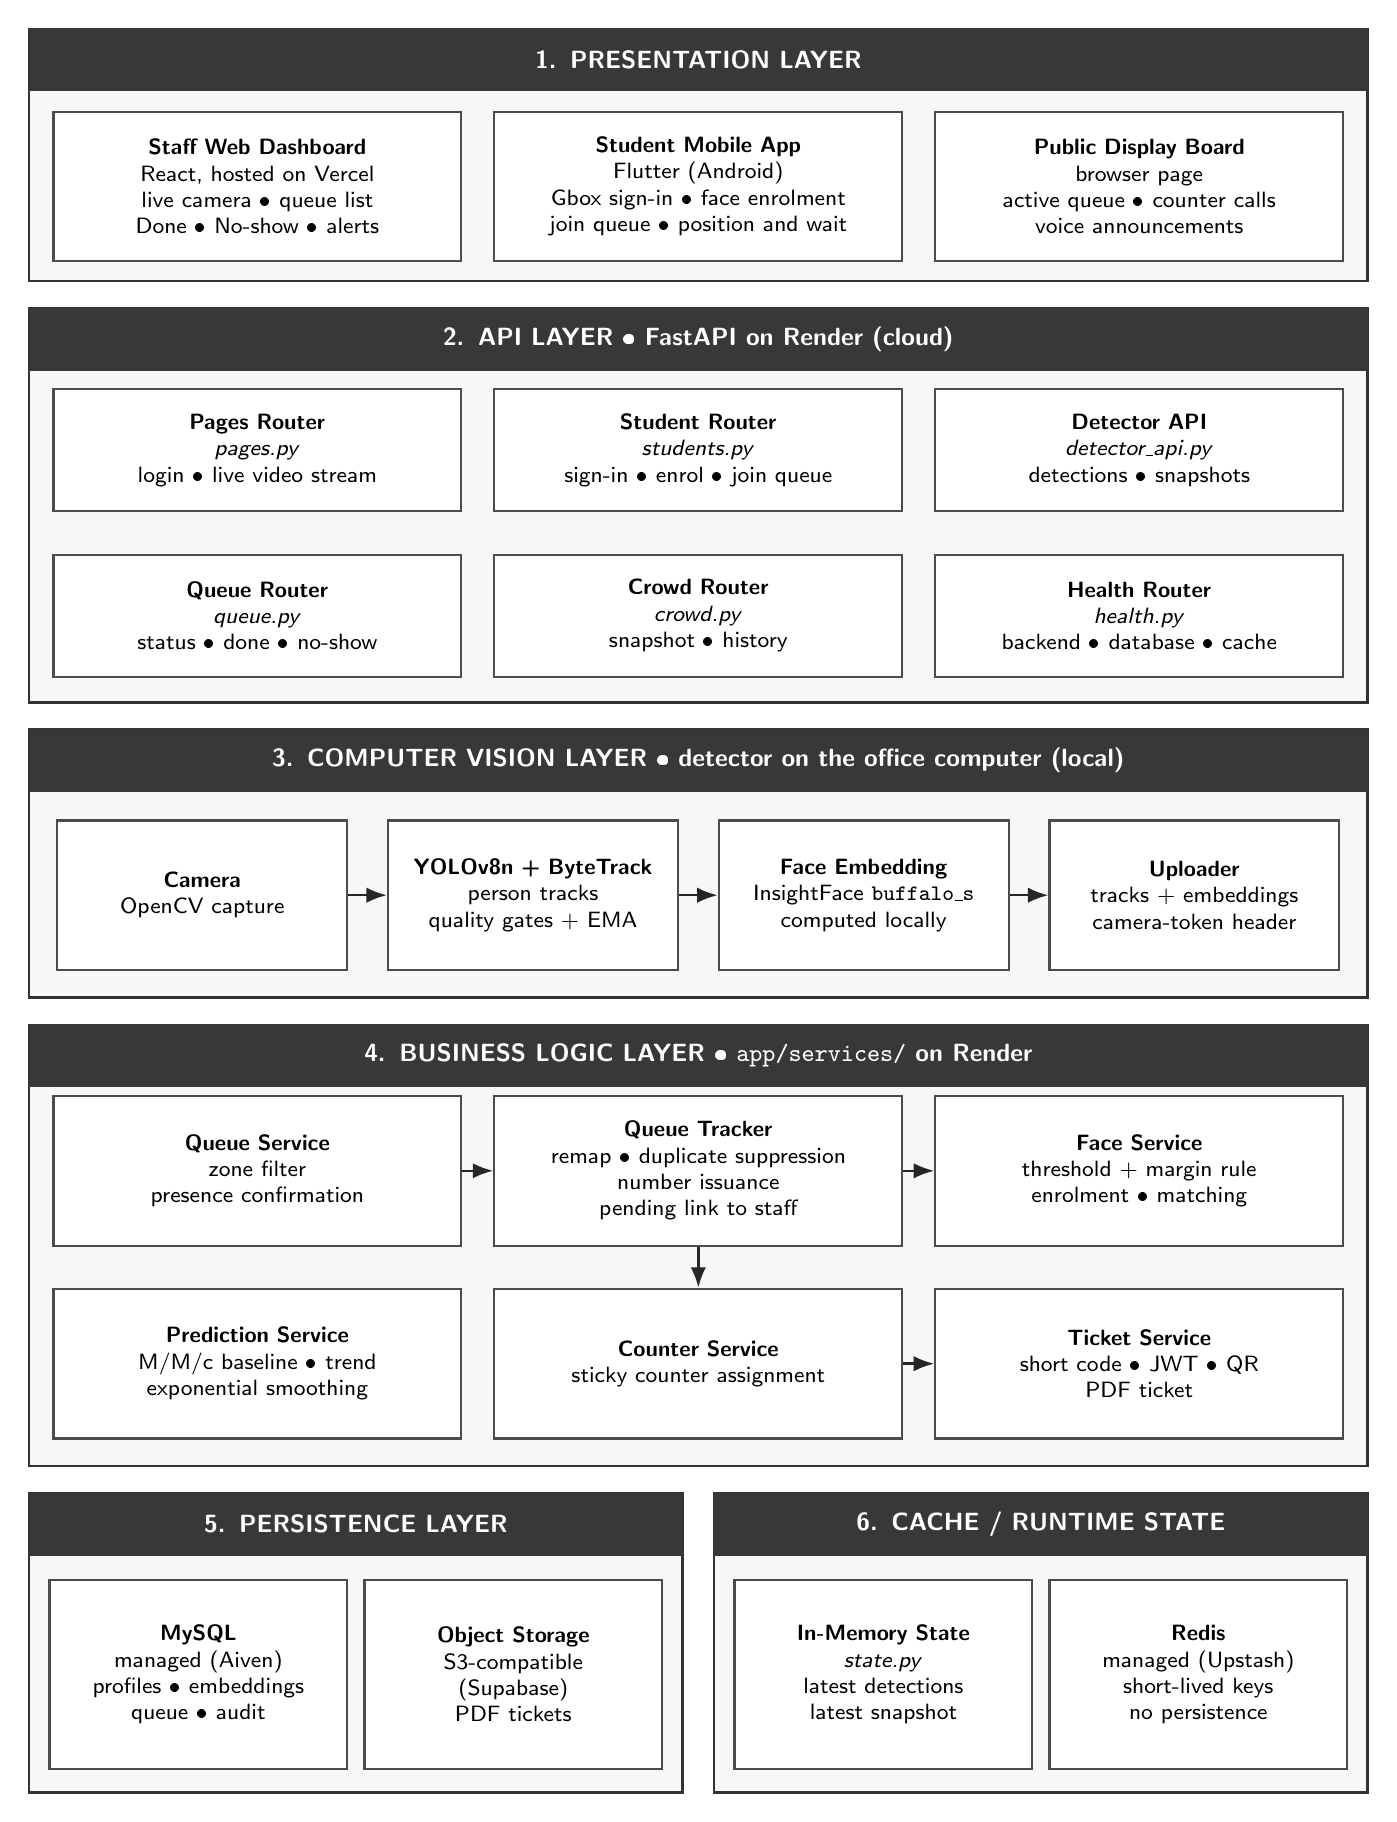
\begin{tikzpicture}[
    font=\sffamily,
    layer/.style={draw=black!80, line width=1pt, fill=black!3,
      minimum width=17cm},
    lhead/.style={fill=black!78, text=white, font=\sffamily\bfseries\small,
      minimum width=17cm, minimum height=0.8cm, anchor=north,
      align=center, inner sep=3pt},
    hhead/.style={lhead, minimum width=8.3cm},
    box/.style={draw=black!70, line width=0.8pt, fill=white, align=center,
      inner sep=4pt, font=\sffamily\footnotesize},
    b3/.style={box, text width=4.9cm, minimum height=1.9cm},
    r3/.style={box, text width=4.9cm, minimum height=1.55cm},
    b4/.style={box, text width=3.4cm, minimum height=1.9cm},
    b2/.style={box, text width=3.5cm, minimum height=2.4cm},
    arrow/.style={-{Latex[length=2.6mm]}, line width=0.9pt, black!85}
  ]
  %---- L1 PRESENTATION ----
  \node[layer, minimum height=3.2cm] (L1) at (0,-1.6) {};
  \node[lhead] at (L1.north) {1.\enspace PRESENTATION LAYER};
  \node[b3] at (-5.6,-2.0)
    {\textbf{Staff Web Dashboard}\\React, hosted on Vercel\\
     live camera \textbullet{} queue list\\Done \textbullet{} No-show \textbullet{} alerts};
  \node[b3] at ( 0.0,-2.0)
    {\textbf{Student Mobile App}\\Flutter (Android)\\
     Gbox sign-in \textbullet{} face enrolment\\join queue \textbullet{} position and wait};
  \node[b3] at ( 5.6,-2.0)
    {\textbf{Public Display Board}\\browser page\\
     active queue \textbullet{} counter calls\\voice announcements};
  %---- L2 API ----
  \node[layer, minimum height=5.0cm] (L2) at (0,-6.05) {};
  \node[lhead] at (L2.north)
    {2.\enspace API LAYER \textbullet{} FastAPI on Render (cloud)};
  \node[r3] at (-5.6,-5.35) {\textbf{Pages Router}\\\textit{pages.py}\\login \textbullet{} live video stream};
  \node[r3] at ( 0.0,-5.35) {\textbf{Student Router}\\\textit{students.py}\\sign-in \textbullet{} enrol \textbullet{} join queue};
  \node[r3] at ( 5.6,-5.35) {\textbf{Detector API}\\\textit{detector\_api.py}\\detections \textbullet{} snapshots};
  \node[r3] at (-5.6,-7.45) {\textbf{Queue Router}\\\textit{queue.py}\\status \textbullet{} done \textbullet{} no-show};
  \node[r3] at ( 0.0,-7.45) {\textbf{Crowd Router}\\\textit{crowd.py}\\snapshot \textbullet{} history};
  \node[r3] at ( 5.6,-7.45) {\textbf{Health Router}\\\textit{health.py}\\backend \textbullet{} database \textbullet{} cache};
  %---- L3 COMPUTER VISION ----
  \node[layer, minimum height=3.4cm] (L3) at (0,-10.6) {};
  \node[lhead] at (L3.north)
    {3.\enspace COMPUTER VISION LAYER \textbullet{} detector on the office computer (local)};
  \node[b4] (camera) at (-6.3,-11.0) {\textbf{Camera}\\OpenCV capture};
  \node[b4] (yolo)   at (-2.1,-11.0) {\textbf{YOLOv8n + ByteTrack}\\person tracks\\quality gates + EMA};
  \node[b4] (embed)  at ( 2.1,-11.0) {\textbf{Face Embedding}\\InsightFace \texttt{buffalo\_s}\\computed locally};
  \node[b4] (upload) at ( 6.3,-11.0) {\textbf{Uploader}\\tracks + embeddings\\camera-token header};
  \draw[arrow] (camera) -- (yolo);
  \draw[arrow] (yolo)   -- (embed);
  \draw[arrow] (embed)  -- (upload);
  %---- L4 BUSINESS LOGIC ----
  \node[layer, minimum height=5.6cm] (L4) at (0,-15.45) {};
  \node[lhead] at (L4.north)
    {4.\enspace BUSINESS LOGIC LAYER \textbullet{} \texttt{app/services/} on Render};
  \node[b3] (qsvc)    at (-5.6,-14.5) {\textbf{Queue Service}\\zone filter\\presence confirmation};
  \node[b3] (tracker) at ( 0.0,-14.5) {\textbf{Queue Tracker}\\remap \textbullet{} duplicate suppression\\number issuance\\pending link to staff};
  \node[b3] (facesvc) at ( 5.6,-14.5) {\textbf{Face Service}\\threshold + margin rule\\enrolment \textbullet{} matching};
  \node[b3] (pred)    at (-5.6,-16.95) {\textbf{Prediction Service}\\M/M/c baseline \textbullet{} trend\\exponential smoothing};
  \node[b3] (counter) at ( 0.0,-16.95) {\textbf{Counter Service}\\sticky counter assignment};
  \node[b3] (ticket)  at ( 5.6,-16.95) {\textbf{Ticket Service}\\short code \textbullet{} JWT \textbullet{} QR\\PDF ticket};
  \draw[arrow] (qsvc)    -- (tracker);
  \draw[arrow] (tracker) -- (facesvc);
  \draw[arrow] (tracker) -- (counter);
  \draw[arrow] (counter) -- (ticket);
  %---- L5 & L6 ----
  \node[layer, minimum width=8.3cm, minimum height=3.8cm] (L5) at (-4.35,-20.5) {};
  \node[hhead] at (L5.north) {5.\enspace PERSISTENCE LAYER};
  \node[b2] at (-6.35,-20.9) {\textbf{MySQL}\\managed (Aiven)\\profiles \textbullet{} embeddings\\queue \textbullet{} audit};
  \node[b2] at (-2.35,-20.9) {\textbf{Object Storage}\\S3-compatible\\(Supabase)\\PDF tickets};
  \node[layer, minimum width=8.3cm, minimum height=3.8cm] (L6) at (4.35,-20.5) {};
  \node[hhead] at (L6.north) {6.\enspace CACHE / RUNTIME STATE};
  \node[b2] at (2.35,-20.9) {\textbf{In-Memory State}\\\textit{state.py}\\latest detections\\latest snapshot};
  \node[b2] at (6.35,-20.9) {\textbf{Redis}\\managed (Upstash)\\short-lived keys\\no persistence};
  \end{tikzpicture}%
  }
  \caption[\sysname{} six-layer system architecture]{\sysname{} Six-Layer
  System Architecture. Layer~3 runs on the office computer attached to
  the camera; all other layers run in the cloud.}
  \label{fig:system-architecture}
\end{figure}

\textbf{Presentation Layer.} This layer has three user-facing surfaces.
The \emph{staff web dashboard}, built in React and hosted on Vercel,
shows the live camera view, the queue list with Done and No-show actions
for each entry, alerts for people the system could not identify, an
emergency manual entry, counter controls, and analytics. The \emph{student mobile application}, built in
Flutter, handles sign-in with the student's NCF Gbox account, voluntary
face enrolment, the request to join the queue, and the student's own
position and estimated wait; it never shows the camera feed or any other
student's status. The \emph{public display board} renders the active
queue in the waiting area and announces counter calls using the
browser's built-in Web Speech API, so no audio leaves the browser.

\textbf{API Layer.} This layer is a FastAPI application hosted on Render
and is organised into six routers. \texttt{pages.py} serves the login
page and the live MJPEG video stream; \texttt{students.py} handles
sign-in, face enrolment, the request to join, and a student's own queue
status; \texttt{detector\_api.py} receives detection metadata and
snapshots from the detector; \texttt{queue.py} serves the queue list,
queue status, prediction, analytics, and the staff actions of marking an
entry done or a no-show; \texttt{crowd.py} serves snapshots and recent
history; and \texttt{health.py} reports the state of the backend,
database, cache, and snapshot feed.

\textbf{Computer Vision Layer.} This layer is a separate Python process
running on the office computer attached to the camera, implemented in
\texttt{app/detector.py}. It reads frames through OpenCV, runs YOLOv8n with
ByteTrack~\cite{zhang2022bytetrack} persistent tracking, and passes each
detection through five quality gates --- minimum bounding-box area,
maximum frame coverage, portrait aspect ratio, motion energy, and
non-maximum suppression --- before smoothing its box with an exponential
moving average. For each tracked person whose face is visible, it then
computes the face embedding locally with InsightFace \texttt{buffalo\_s}.
Only the resulting metadata --- tracks, boxes, and embeddings --- and a
compressed snapshot for the live view are sent to the backend, over
requests authenticated by a camera token. Running the detector as its
own process keeps camera work from blocking the dashboard or the API.
Gate thresholds and the smoothing factor are specified in
Section~\ref{subsec:cv-layer}.

\begin{figure}[!htbp]
  \centering
  \resizebox{!}{0.86\textheight}{%
  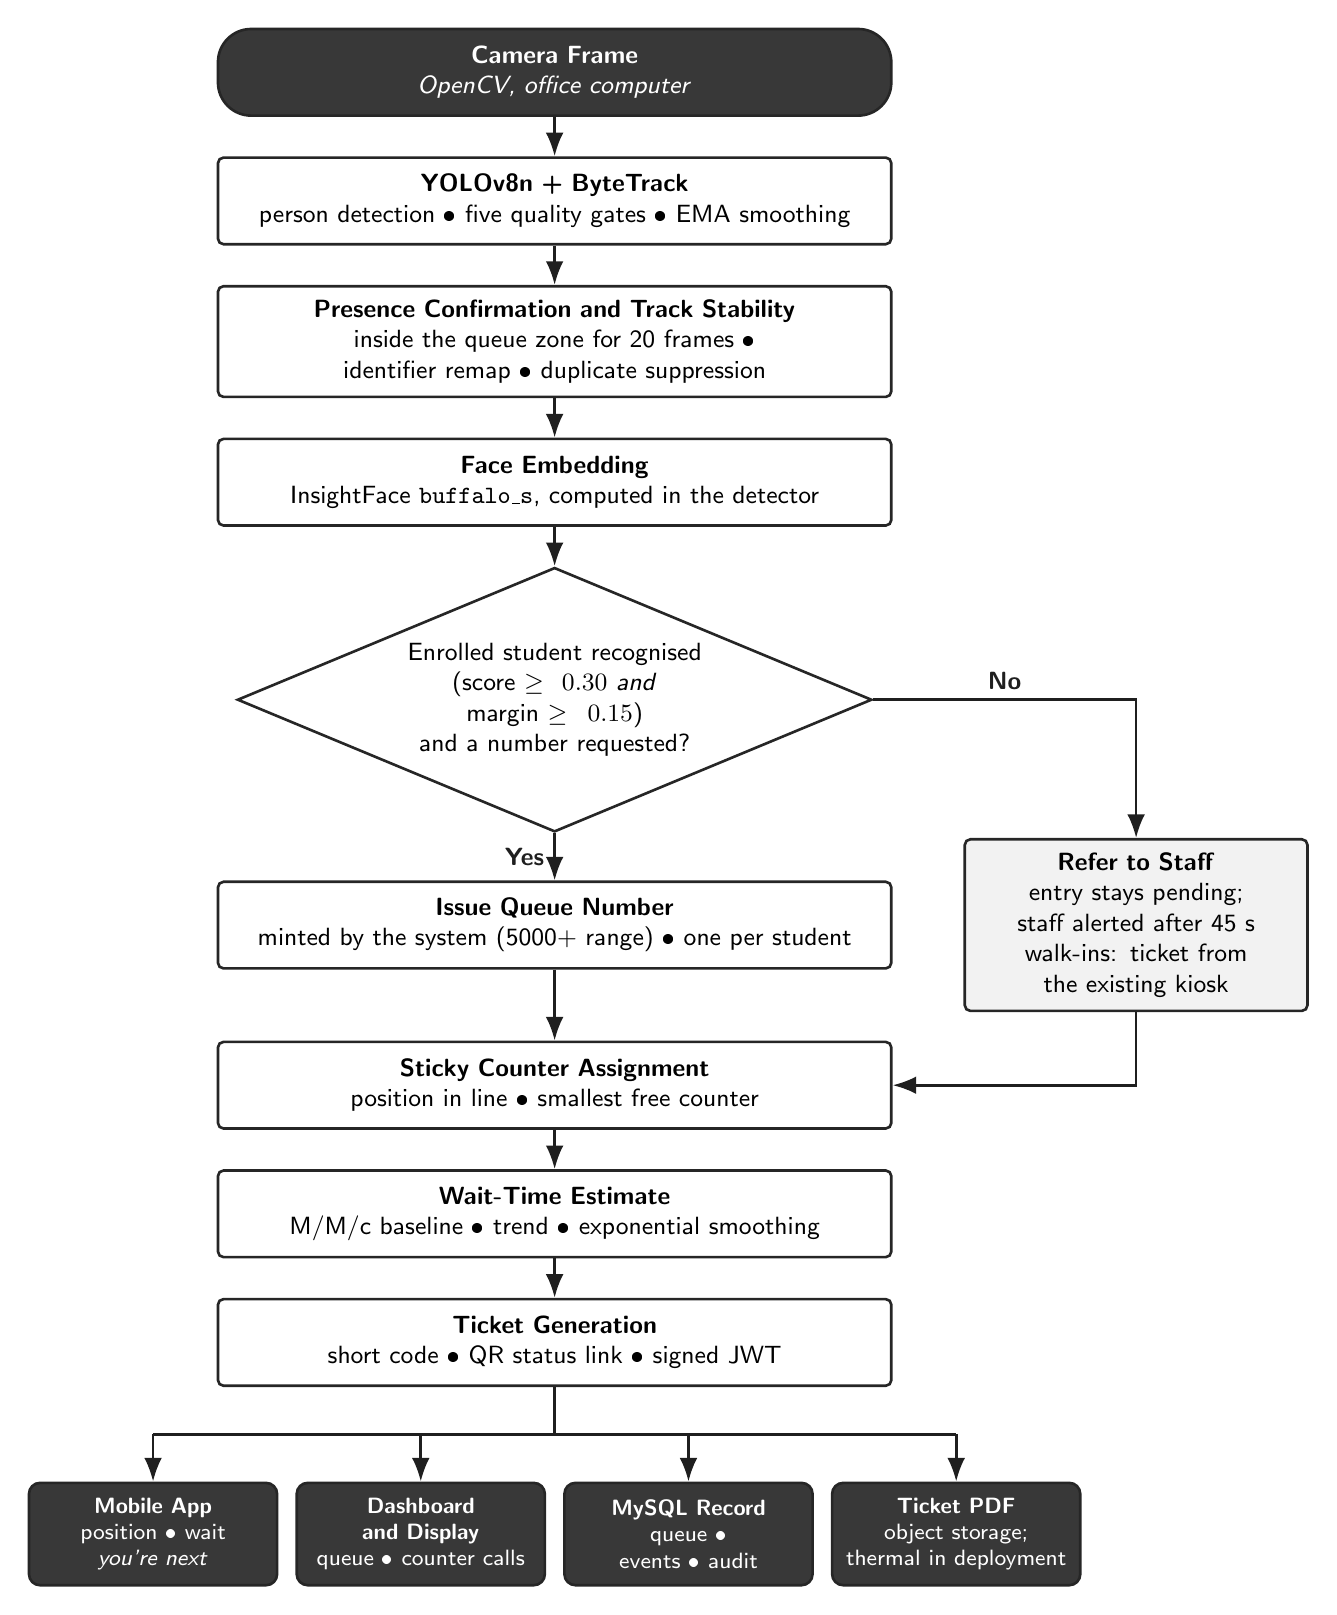
\begin{tikzpicture}[
    font=\sffamily,
    node distance=0.5cm,
    proc/.style={draw=black!85, line width=0.95pt, fill=white, align=center,
      rounded corners=2pt, text width=8.2cm, minimum height=1.1cm,
      inner sep=5pt, font=\sffamily\small},
    dark/.style={proc, fill=black!78, text=white, rounded corners=12pt},
    side/.style={proc, text width=4.0cm, fill=black!5},
    decision/.style={diamond, aspect=2.4, draw=black!85, line width=0.95pt,
      fill=white, align=center, text width=4.6cm, inner sep=0pt,
      font=\sffamily\small},
    outbox/.style={proc, fill=black!78, text=white, text width=2.8cm,
      minimum height=1.3cm, rounded corners=4pt, font=\sffamily\footnotesize},
    arrow/.style={-{Latex[length=3mm]}, line width=0.95pt, black!88},
    lab/.style={font=\sffamily\small\bfseries}
  ]
  \hyphenpenalty=10000
  \exhyphenpenalty=10000
  \node[dark] (camera) at (0,0)
    {\textbf{Camera Frame}\\\textit{OpenCV, office computer}};
  \node[proc, below=of camera] (detect)
    {\textbf{YOLOv8n + ByteTrack}\\person detection \textbullet{} five quality gates \textbullet{} EMA smoothing};
  \node[proc, below=of detect] (zone)
    {\textbf{Presence Confirmation and Track Stability}\\inside the queue zone for 20 frames \textbullet{} identifier remap \textbullet{} duplicate suppression};
  \node[proc, below=of zone] (embed)
    {\textbf{Face Embedding}\\InsightFace \texttt{buffalo\_s}, computed in the detector};
  \node[decision, below=of embed] (dec)
    {Enrolled student recognised\\(score $\geq 0.30$ \emph{and}\\margin $\geq 0.15$)\\and a number requested?};
  \node[proc, below=0.6cm of dec] (issue)
    {\textbf{Issue Queue Number}\\minted by the system (5000+ range) \textbullet{} one per student};
  \node[side, right=0.9cm of issue] (staff)
    {\textbf{Refer to Staff}\\entry stays pending; staff alerted after 45~s\\walk-ins: ticket from the existing kiosk};
  \node[proc, below=0.9cm of issue] (counter)
    {\textbf{Sticky Counter Assignment}\\position in line \textbullet{} smallest free counter};
  \node[proc, below=of counter] (predict)
    {\textbf{Wait-Time Estimate}\\M/M/c baseline \textbullet{} trend \textbullet{} exponential smoothing};
  \node[proc, below=of predict] (ticket)
    {\textbf{Ticket Generation}\\short code \textbullet{} QR status link \textbullet{} signed JWT};

  \foreach \a/\b in {camera/detect, detect/zone, zone/embed, embed/dec, issue/counter, counter/predict, predict/ticket}
    \draw[arrow] (\a) -- (\b);
  \draw[arrow] (dec) -- node[lab, left] {Yes} (issue);
  \draw[arrow] (dec.east) -| node[lab, above, pos=0.25] {No} (staff.north);
  \draw[arrow] (staff.south) |- (counter.east);

  % outputs
  \node[outbox, below=1.2cm of ticket, xshift=-5.1cm] (o1) {\textbf{Mobile App}\\position \textbullet{} wait\\\emph{you're next}};
  \node[outbox, below=1.2cm of ticket, xshift=-1.7cm] (o2) {\textbf{Dashboard and Display}\\queue \textbullet{} counter calls};
  \node[outbox, below=1.2cm of ticket, xshift= 1.7cm] (o3) {\textbf{MySQL Record}\\queue \textbullet{} events \textbullet{} audit};
  \node[outbox, below=1.2cm of ticket, xshift= 5.1cm] (o4) {\textbf{Ticket PDF}\\object storage;\\thermal in deployment};
  \draw[line width=0.95pt, black!88] (ticket.south) -- ++(0,-0.6) coordinate (sp);
  \draw[line width=0.95pt, black!88] (o1.north |- sp) -- (o4.north |- sp);
  \foreach \o in {o1,o2,o3,o4}
    \draw[arrow] (\o.north |- sp) -- (\o.north);
  \end{tikzpicture}%
  }
  \caption[\sysname{} detection-to-ticket pipeline]{\sysname{}
  Detection-to-Ticket Pipeline. Only an enrolled student who is
  recognised with confidence and has asked for a number is issued one by
  the system; every other person is referred to staff. Walk-ins take a ticket from the
  office's existing kiosk, which runs separately from the system.}
  \label{fig:detection-ticket-pipeline}
\end{figure}

\textbf{Business Logic Layer.} This layer is implemented in
\texttt{app/services/} and runs on Render with the API. The \emph{Queue
Service} removes weak detections, applies the centroid-in-rectangle zone
test (\S\ref{subsec:candidate}), and passes confirmed detections to the
Queue Tracker. The \emph{Queue Tracker} holds the active queue in memory;
confirms presence through a 20-frame buffer with a motion check
(\S\ref{subsec:candidate}); keeps tracks stable through identifier
remapping (\S\ref{subsec:remap}) and duplicate suppression with re-entry
immunity (\S\ref{subsec:dedup}); and, through the \emph{Face Service},
compares each confirmed person's embedding with the enrolled roster under
the threshold-and-margin rule (\S\ref{subsec:reid}). A queue number is
issued only to an enrolled student who is recognised with confidence
and has asked for a number in the mobile application; anyone else stays
unlinked, and after 45~seconds the dashboard alerts staff
(Figure~\ref{fig:detection-ticket-pipeline}). Walk-ins are not handled
here at all: they take a ticket from the office's existing kiosk, which
runs separately from \sysname{}. The tracker then produces
the sticky counter assignments shown on the dashboard
(\S\ref{subsec:counters}).

\textbf{Emergency manual entry.} The dashboard also gives staff a manual
override for the occasions when automatic recognition cannot do its job:
the camera is blocked or offline, the detector has stopped, or a
registered student is standing in the queue but cannot be recognised,
for example because of poor lighting or a face covering. Staff can use
it in two ways. A person the camera sees but could not identify, shown
among the pending-link alerts, can be given a queue number directly; and
when the camera cannot see the person at all, staff can type a queue
number to create the entry by hand. A manual entry joins the queue in the
same order as any other, receives a counter and a ticket in the usual
way, and stays in the queue until staff mark it done or a no-show, since
there is no camera track that could expire. The system refuses any
number already issued that day, so manual entry cannot create a
duplicate. This is an emergency feature, not part of the normal flow, and
every entry made through it is recorded as manual; how often staff
needed it is therefore itself evidence of how often automatic
recognition fell short. Because the dashboard runs in the cloud, the
override covers a failure of the camera or of recognition, but not a loss
of the office's internet connection.

The \emph{Prediction Service} runs four sub-models in sequence on a
rolling buffer of crowd-count samples: an M/M/c queueing baseline for
the current wait estimate (\S\ref{subsubsec:mmc-baseline}); a linear
trend-projection forecast at the five-minute horizon
(\S\ref{subsubsec:short-forecast}); Holt's double-exponential
smoothing forecast at the fifteen-minute horizon
(\S\ref{subsubsec:holt-forecast}); and a growth-ratio mean-reversion
forecast at the thirty-minute horizon (\S\ref{subsubsec:long-forecast}).
The arrival rate $\lambda$ is estimated from the difference of recent
queue counts (\S\ref{subsubsec:arrival-rate}); the service rate $\mu$
is supplied by the dynamic service-time measurement described in
Section~\ref{subsec:service-time}, which recomputes the average service
time every five minutes from the transaction log.

The \emph{Counter Service} allocates counters using a sticky-assignment
rule: each frame, the active queue is sorted by queue number, each person
receives a position in line, and each unassigned person at a position no
greater than the number of open counters is given the smallest free
counter number. An allocation persists until the entry is marked done or
a no-show (\S\ref{subsec:counters}).

The \emph{Ticket Service} is a background worker that consumes
ticket-generation jobs. The \emph{Ticket Printer} produces the short
code, the JSON Web Token signed with HMAC-SHA256, the QR-encoded status
URL, and the PDF ticket, which is stored in object storage; in the
deployment configuration it drives a thermal printer instead. The short
code is drawn from a 32-character alphabet that excludes the ambiguous
characters 0, O, 1, and I, and is formatted as \texttt{XXXX--XXXX}. The
JWT carries a four-hour expiry and a 32-hex-digit nonce to prevent
replay. The complete payload specification is in
Section~\ref{subsec:ticket}.

\textbf{Persistence Layer.} This layer is a managed MySQL database hosted
on Aiven, accessed through \texttt{app/database/database\_handler.py},
together with S3-compatible object storage on Supabase for PDF tickets.
The database holds student profiles and their face embeddings, queue
records with their short codes, tokens, statuses, and timestamps,
operational events, and the audit of every recognition decision. Raw
camera frames, live snapshots, enrolment photographs, and the in-memory
queue state are intentionally never persisted.

\textbf{Cache and Runtime State Layer.} This layer comprises an in-memory
state module, \texttt{app/state.py}, holding the latest detector output,
the latest annotated snapshot, and a short rolling history, and a managed
Redis cache on Upstash, accessed through
\texttt{app/services/cache\_service.py}, which shares live values
between backend workers. The cache is volatile by design: every key
carries a short time-to-live and nothing in it is written to disk as a
record of the queue.


\subsection{Dynamic Service-Time Measurement}
\label{sec:dynamic-service-time-method}

\sysname{} treats average service time as a value that can change
during live operation, not as a fixed assumption decided before
deployment. Every five minutes, a background measurement routine reads
recent completed transactions from the MySQL log and estimates the
current service pace from inter-departure gaps. For completed
transaction timestamps $t_1, t_2, \ldots, t_N$, each gap is computed in
minutes as

\begin{equation}
g_i = \frac{t_i - t_{i-1}}{60}, \qquad i = 2, \ldots, N.
\label{eq:method-svc-gap}
\end{equation}

\noindent Gaps below 0.1 minute are treated as database-write noise,
while gaps above 15 minutes are treated as idle periods rather than
normal cashier service. The retained gaps are averaged and multiplied
by the number of active counters to account for parallel service. The
new estimate is then blended with the previously stored value:

\begin{equation}
\widehat{\mathrm{svc}}_{\text{new}} =
0.7\,\widehat{\mathrm{svc}} +
0.3\,\widehat{\mathrm{svc}}_{\text{prev}}.
\label{eq:method-svc-blend}
\end{equation}

\noindent This dynamic measurement supplies the service rate $\mu$ used
by the prediction module after the system has recorded enough
transactions. The pre-deployment service-time calibration in
Section~\ref{sec:datagathering} is therefore used only as the initial
seed value.

\subsection{Machine-Learning Wait-Time Predictor Training Protocol}
\label{sec:ml-training-protocol}

\sysname{} does not train its wait-time model while the cashiering
prototype is already serving users. Training is handled as an offline
step: the researchers prepare the transaction logs, test several
predictors on past records, and deploy the selected model only after
its error values are acceptable for the study. This keeps experimental
model changes away from live queue operations and gives the researchers
a reproducible basis for the results presented later in the manuscript.

\textbf{Dataset.} The working dataset comes from historical cashiering
queue logs made available for \sysname{} predictor development. The XML
export contains 49,303 queue records covering March~24,~2023 to
May~4,~2026. The available fields include queue identifier, application
identifier, queue number, service date, service time, transaction type,
processing status, and program identifier. Names, student numbers,
payment amounts, account details, and other personally identifiable
fields are not used by the model. Records marked with
\texttt{processing = 3} are excluded because they represent no-show,
cancelled, or incomplete queue events.

\textbf{Feature Engineering.} The predictor uses three feature groups.
The first group is derived directly from the queue logs and timestamp
sequence:
\begin{enumerate}
  \item Queue and transaction fields: queue number, transaction type,
        program identifier, daily queue size, and estimated people
        ahead.
  \item Time fields: hour, minute, day of week, month, morning or
        afternoon indicator, and peak-hour indicator.
  \item Recent-demand fields: arrivals within the previous 5 and
        15 minutes.
\end{enumerate}
The second group consists of academic-period indicators for enrollment,
prelim, midterm, final, and clearance periods. These indicators allow
the model to distinguish ordinary service days from predictable
cashiering-demand spikes.

The third group grounds the AI model in the analytical prediction
framework of \sysname{}. For every training row, the preparation script
computes outputs from the mathematical routines described in
Section~\ref{subsec:prediction}: an M/M/c-style baseline wait, a
local trend-projected wait, a Holt double-exponential smoothing
estimate, a growth-ratio mean-reversion estimate, the estimated
arrival rate, and the estimated service time. These analytical outputs
are used as input features to the machine-learning model rather than
as replacements for it.

The response variable is reconstructed wait time in minutes. Because
the XML export does not contain both a queue-entry timestamp and a
counter-arrival timestamp for every record, wait time is reconstructed
as the elapsed time from a valid queue record to the next valid served
record on the same service date. Reconstructed waits below one minute
are excluded during model fitting because sub-minute gaps may represent
immediate transaction encoding or log artifacts rather than meaningful
queue waiting. Reconstructed waits above 120 minutes are excluded to
avoid idle-period outliers.

\textbf{Train and Test Split.} Queue records are split by service date,
not by random row assignment. The first 80\% of ordered service dates
form the training set and the remaining 20\% form the test set. This
order matters because cashiering demand is time-dependent: enrollment
week, payment deadlines, and ordinary class days do not behave the same
way. A random split could allow future queue patterns to influence
model tuning, so it is avoided.

\textbf{Model Architecture.} The implemented AI component uses
Gradient Boosting Regression through scikit-learn's
\texttt{HistGradientBoostingRegressor}. Gradient boosting is selected
because the available data is tabular and contains mixed operational,
calendar, and analytical prediction features. The model learns
nonlinear corrections from historical queue behavior while still being
anchored to the interpretable mathematical estimates computed by the
prediction service.

Deep sequence models such as Long Short-Term Memory networks and the
Temporal Fusion Transformer are not used in this version of the
prototype. These architectures may be useful for large, multi-office
time-series datasets, but the available cashiering data comes from a
single service office. For this study, simpler tabular models are more
appropriate and easier to validate.

\textbf{Hyperparameter Selection.} The prototype model uses 300
boosting iterations, a learning rate of 0.05, 31 maximum leaf nodes,
and L2 regularization of 0.1. These conservative settings were chosen
to keep the model stable on the reconstructed wait-time target and to
avoid overfitting to short timestamp gaps.

\textbf{Evaluation Protocol.} The selected model is evaluated on the
date-based held-out test set using MAE, RMSE, MAPE, and $R^2$. MAE and
RMSE are treated as the primary metrics because reconstructed waits can
be short, making percentage-based error unstable. MAPE is still
reported for transparency but is interpreted cautiously.

\textbf{Integration Plan.} After offline testing, the trained model is
serialized with \texttt{joblib} and loaded by the FastAPI backend at
startup. During a ticket-status request, the backend computes the live
feature vector, including queue-state features, academic-period
features, and the analytical prediction features described above. The
Gradient Boosting prediction is then calibrated with current-day
service speed, yesterday's same-hour wait behavior, and recent
prediction error before being returned to the dashboard or student
status page as the displayed wait-time estimate.

\textbf{Retraining and Model Drift.} The procedure in this subsection
covers the initial training run only. Periodic retraining, automated
drift monitoring, and production retraining pipelines are outside the
present scope, although the prototype is arranged so that a later model
file can replace the original one. The resulting training metrics are
reported in Chapter~3.

\section{Software Development Process}
\label{sec:sdp}

\sysname{} development is organized as a small Agile-style engineering
cycle. Requirements, interface decisions, coding work, testing, and
review are repeated across modules instead of being handled as one
large build at the end of the study.

\textbf{Planning and Requirement Analysis.} The researchers will
collaborate with NCF service office staff to determine system
requirements. User needs, expected workflows, dashboard actions, and
ticket conventions will be documented to create user stories,
prioritize features, and align development goals with the conceptual
framework presented in Chapter~1.

\textbf{System Design.} This phase focuses on the architecture and
design of the detection pipeline, the backend, the database, and the
dashboard. It includes queue-zone coordinate design, ticket-payload
schema design, prediction-module parameter design, and dashboard
wireframing.

\textbf{Development Iteration and Sprint Cycles.} Development is
organized into sprint cycles, each concentrating on a specific module.
The sprints, in the order in which they will be executed, are
summarized below:
\begin{enumerate}
  \item YOLOv8n pipeline setup, queue-zone configuration, and the
        custom NMS pre-filter for duplicate head and body box
        suppression.
  \item Hybrid re-entry matching algorithm design, implementation, and
        iterative debugging using recorded test footage.
  \item Queue position recalculation logic.
  \item Prediction module implementation of the M/M/c baseline,
        short-term trend projection, Holt smoothing, and
        mean-reversion long forecast; iterative accuracy tuning against
        logged ground-truth wait times.
  \item FastAPI backend, staff web dashboard, and counter controls.
  \item Printer-agnostic ticket workflow, including JWT issuance,
        short-code generation, QR linking, and PDF rendering for
        demonstration.
  \item Student status integration, including mobile client, status
        API, and end-to-end ticket scan tests.
  \item Integration testing, performance tuning, and final
        pre-evaluation hardening.
\end{enumerate}

Each of the eight sprints listed above is executed through a five-phase
cycle: Plan, Design, Build, Test, and Review. Sprint-level Plan and
Design refine the module's acceptance criteria and interface contracts
before Build; Test validates the deliverable against those criteria;
and Review captures adviser feedback together with measured performance,
which then propagates into the Plan phase of the following sprint.
This per-sprint feedback loop instantiates, at the development level,
the Feedback stage described in the conceptual framework of
Section~\ref{sec:conceptual-framework}.

% Figure 2.3 removed per panel recommendation.
% The Agile cycle figure should only be included if customized
% to show \sysname{}-specific stages and phases.
% Reinsert the figure block below once a study-specific version is prepared.
%
% \begin{figure}[!htbp]
%   \centering
%   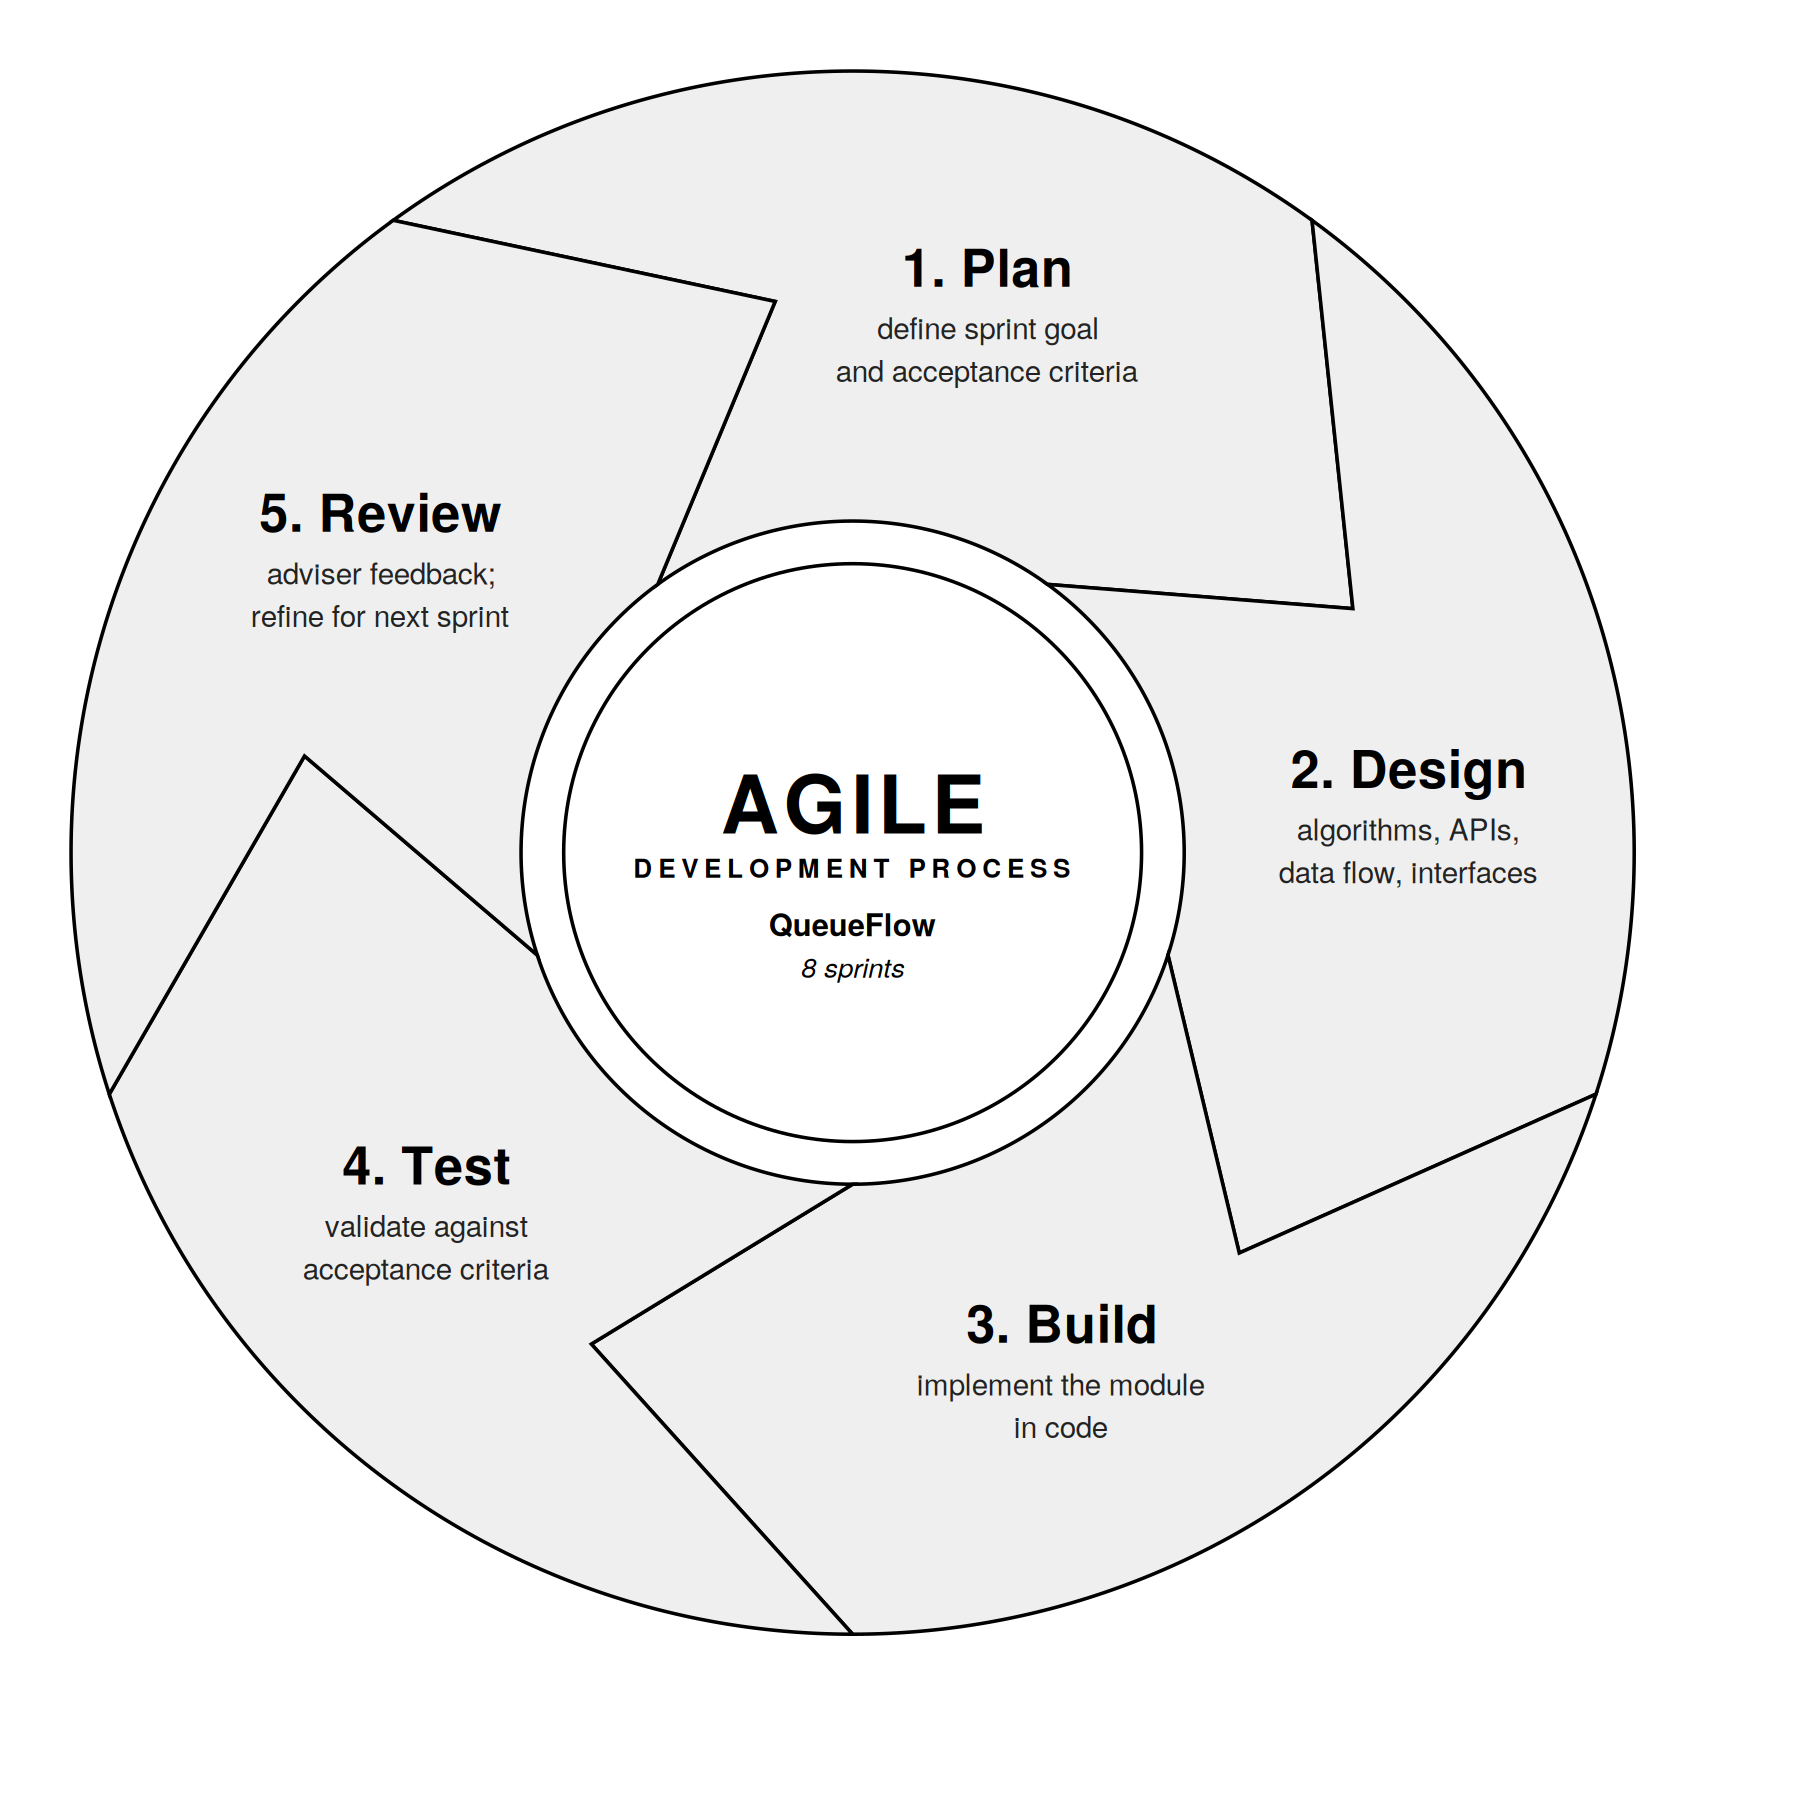
\includegraphics[width=0.78\textwidth,height=0.74\textheight,keepaspectratio]{queueflow_agile_cycle.png}
%   \par\vspace{0.3em}{\centering\small\textbf{Figure 2.3}\par}
%   \caption{Agile Development Process for \sysname{}.}
%   \label{fig:agile-cycle}
% \end{figure}

Each sprint will conclude with a review against defined acceptance
criteria and with the thesis adviser before proceeding to the next
phase. Sprint reviews will also be used to refine prediction parameters
and queue-zone calibration based on observed system behavior,
consistent with the feedback loop described in Section~1.6 of
Chapter~1.

\section{Validation and Testing Methods}
\label{cr:validation}

Validation combines software tests, observed performance, and user
feedback. Functional and integration tests check whether the prototype
works as intended; queue assignment, re-identification, prediction, and
latency measures address the technical research questions; and the
survey and interviews address user evaluation.

\textbf{Alpha Testing.} Alpha testing will be conducted internally by
the developers using both live camera input and pre-recorded test
footage. Defects in detection, tracking, ticket generation, dashboard
rendering, and mobile-client status retrieval will be identified and
resolved before any external user is exposed to the system.

\textbf{Beta Testing.} Under the shortened evaluation protocol, beta
testing takes the form of a supervised trial session in which NCF
service staff operate the system while volunteer students use it. The
developers observe the interaction and log any operational issues, and
the same session provides the structured evaluation described below,
rather than following a separate two-week period of regular
operation.

\textbf{Performance Testing: Queue Assignment Accuracy.} During defined
observation windows, an independent observer will maintain a manual
ground-truth log in which every actual queue entrant will be recorded
with a timestamp. The system's queue assignments will then be compared
against this log. Accuracy is reported as the proportion of correct
assignments over total arrivals, using the formula in Section~2.7.

\textbf{Performance Testing: Re-Identification Reliability.} Re-entry
events, in which a tracked person leaves the camera frame and later
returns, will also be recorded in the same manual ground-truth log. The
system's re-entry decision, either assigning a new number or restoring
a previous number, will be compared against the ground-truth identity
recorded by the observer. Reliability is reported as the proportion of
correct decisions over total re-entry events.

\textbf{Performance Testing: Prediction MAE and MAPE.} Actual wait
times will be measured by the observer using a stopwatch from the
moment a person enters the queue zone to the moment the person reaches
the counter. These observed wait times will be compared to the
system's predictions at the corresponding horizons. MAE and MAPE will
be computed using the formulas in Section~2.7, separately for the
current, 5-minute, 15-minute, and 30-minute horizons.

\textbf{Performance Testing: Latency and Ticket Flow.}
Detection-to-ticket latency will be measured from automated timestamps
logged at the moment a queue entrant is first detected, that is, the
moment the detection passes all five quality gates of the Computer
Vision Layer (\S\ref{subsec:cv-layer}), to the moment the
corresponding ticket payload is issued after candidate confirmation and
queue-number assignment. Ticket flow validation will be performed by
issuing tickets across a representative range of conditions and
verifying that the short code, QR link, and JWT each correctly resolves
to the matching queue status. Failures will be logged and counted
toward the ticket and token validation rate reported under Statement of
the Problem No.~2.

\textbf{Usability Evaluation.} Immediately after the supervised trial
session, the content-validated questionnaire in Section~2.5 is
administered to the respondent groups identified in Section~2.3.
Because the questionnaire is researcher-made, its internal-consistency
reliability is measured with Cronbach's alpha on those responses, with a
value of at least $0.70$ taken as acceptable, as specified in
Section~2.5. The baseline
questionnaire for Statement of the Problem No.~1 is also researcher-made
and was tested in the same way; its coefficients are reported with the
results in Section~\ref{sec:sop1-results}. Responses will
be analyzed using the statistical procedures in Section~2.7. A subset
of respondents from each group will be invited to a short
semi-structured interview, and the resulting transcripts will be
thematically coded to surface patterns that the Likert ratings alone
do not capture.

\textbf{Load and Pressure Testing.} To assess system stability under
concurrent user load, load and pressure testing will be conducted
before deployment. The testing will simulate multiple simultaneous
connections to the FastAPI backend, including concurrent detector
uploads, dashboard polling requests, and student status queries. The
primary metrics are response time under load, error rate, and system
recovery behavior when traffic exceeds normal operational levels.
Findings from load testing are used to identify and address
performance bottlenecks before the evaluation period begins.

The combination of automated performance logs, manual ground-truth
observation, structured survey responses, qualitative interviews, and
load testing provides multiple lines of evidence for each research
question, supporting the convergent parallel mixed-methods design
described in Section~2.1.

% ============================================================
% CHAPTER 3: RESULTS AND DISCUSSIONS
% ============================================================
\chapter{Results and Discussions}

% ----------------------------------------------------------------
% 3.1  SOP #1 — Current limitations of manual queue management
% ----------------------------------------------------------------
\section[Current Problems with the Manual Queue Management Process]{Current Problems with the Manual Queue\\ Management Process}
\label{sec:sop1-results}

This section addresses Statement of the Problem No.~1: \emph{What are
the current problems with the manual queue management process during
busy periods, regarding wait times and user-experience?} The findings
are drawn from the pre-deployment baseline survey administered during
Phase~1 of the data-gathering procedure described in
Section~\ref{sec:datagathering}, using the instrument described in
Section~\ref{sec:instrument}.

Twenty-two respondents completed the survey: 15 students and 7 staff
members of the service office. Among the staff, 6 handle queue
transactions daily and 4 have done so for one to three years. Among the
students, 10 are in their fourth year and 12 use the office
occasionally or rarely rather than daily, which matters for
interpretation: these are not people whose answers reflect a single bad
day, but the ordinary experience of an occasional visitor.

The two groups answered different items against the same five-point
scale --- staff about running the queue, students about waiting in it
--- so their results are reported side by side rather than pooled.
Every item is worded as a problem, so agreement means the problem is
real. For this reason only the agreement half of Table~\ref{tab:likert}
is used here; its quality half reads backwards on a problem statement,
where agreeing is the unfavourable outcome.

Because the questionnaire is researcher-made, its internal consistency
was tested with Cronbach's alpha before the results were interpreted
(Table~\ref{tab:sop1-reliability}). The student form is reliable as a
whole ($\alpha = 0.857$) and in both sections. The staff form is
acceptable as a whole ($\alpha = 0.796$) and in its user-experience
section, but its wait-time section is not ($\alpha = 0.288$): the seven
staff agreed strongly with some wait-time items and disagreed with
others, so the items do not move together. With seven respondents this
coefficient is also unstable. The staff wait-time section weighted mean
is therefore reported as a descriptive average only, and the staff
findings below are interpreted item by item rather than as a composite.

\begin{table}[H]
\centering
\caption{Internal consistency of the baseline questionnaire
(Cronbach's alpha).}
\label{tab:sop1-reliability}
\begin{tabular}{lccc}
\hline
Form & Wait-time & User experience & Whole form \\
\hline
Students ($n = 15$) & $0.703$ & $0.828$ & $0.857$ \\
Staff ($n = 7$) & $0.288$ & $0.767$ & $0.796$ \\
\hline
\multicolumn{4}{l}{\footnotesize Seven items per section, fourteen per
form. $\alpha \geq 0.70$ is taken as acceptable.} \\
\end{tabular}
\end{table}

\subsection{Problems Reported by Students}
\label{subsec:sop1-students}

Students returned an overall weighted mean of $4.25$ (\emph{Strongly
Agree}), the strongest agreement recorded anywhere in this study.
Table~\ref{tab:sop1-students} gives the item-level results.

\begin{table}[H]
\centering
\caption{Problems with the current queue process as reported by
students ($n = 15$).}
\label{tab:sop1-students}
\begin{tabular}{p{0.66\textwidth}cc}
\hline
Item & WM & Interpretation \\
\hline
\multicolumn{3}{l}{\textbf{Perceived problems on wait-time}} \\
The display shows only the number being served, not how long I still
  need to wait & $4.60$ & Strongly Agree \\
I have experienced long wait times during busy periods & $4.60$ & Strongly Agree \\
I have no way of knowing my estimated wait time after getting my ticket
  & $4.13$ & Agree \\
I need to keep watching the display to know when my number will be
  called & $4.47$ & Strongly Agree \\
I have missed my turn because I was not near the display & $3.47$ & Agree \\
Waiting time feels unpredictable, especially during busy periods & $4.27$ & Strongly Agree \\
Long or unpredictable waits discourage me from availing services at
  peak hours & $4.53$ & Strongly Agree \\
\hline
\multicolumn{2}{l}{\textbf{Section weighted mean}} & $4.30$ \\
\hline
\multicolumn{3}{l}{\textbf{Perceived problems on user experience}} \\
It is inconvenient to have to watch the screen or ask staff to know my
  status & $4.13$ & Agree \\
I get confused whether a window is closed, on break, or not yet open & $4.07$ & Agree \\
I feel frustrated when I do not know how many people are ahead of me & $4.40$ & Strongly Agree \\
There is no notification to tell me when my turn is near & $4.00$ & Agree \\
It is inconvenient to wait without knowing how much time is left & $4.47$ & Strongly Agree \\
The lack of a wait-time estimate affects my overall experience & $4.40$ & Strongly Agree \\
Overall, I am dissatisfied with the current queue process & $4.00$ & Agree \\
\hline
\multicolumn{2}{l}{\textbf{Section weighted mean}} & $4.21$ \\
\hline
\multicolumn{2}{l}{\textbf{Overall weighted mean}} & $\mathbf{4.25}$ \\
\hline
\end{tabular}
\end{table}

\noindent Three items sit at or above $4.47$ and describe the same
condition from different angles: the student cannot see how long the
wait will be, cannot see how many people are ahead, and must therefore
stay within sight of the display. The highest-scoring item on the
user-experience side is not dissatisfaction in general ($4.00$) but the
specific inconvenience of waiting without knowing how much time is left
($4.47$). What the students object to is not the waiting; it is the
\emph{blindness} of the waiting.

The consequence appears in the item scoring $4.53$: long or
unpredictable waits discourage students from availing services during
peak hours. The current process does not merely inconvenience students;
it changes when --- and whether --- they come at all.

The open-ended responses point the same way while adding two problems
the Likert items did not ask about. One student wrote that there is
``no way of telling if the queue is long if I'm not physically present
in the office,'' which is the remote-visibility problem stated plainly.
Two reported being cut in line, one of them ``whenever my turn is near
and told to go back again the next office hours.'' One raised a
physical constraint outside the scope of any software: ``the lack of
waiting space or room for people waiting in line, often times I am
stuck standing in a hallway.'' Another asked for ``guidance of where I
should queue.'' These last three are recorded here because they were
volunteered, but a queue-management system does not solve them.

\subsection{Problems Reported by Staff}
\label{subsec:sop1-staff}

Staff returned an overall weighted mean of $3.34$ (\emph{Neutral}) ---
substantially lower than the students, and the more informative result
of the two. Table~\ref{tab:sop1-staff} gives the item-level figures.

\begin{table}[H]
\centering
\caption{Problems with the current queue process as reported by staff
($n = 7$).}
\label{tab:sop1-staff}
\begin{tabular}{p{0.66\textwidth}cc}
\hline
Item & WM & Interpretation \\
\hline
\multicolumn{3}{l}{\textbf{Perceived problems on wait-time}} \\
The display shows only the number being served, not how long a client
  still needs to wait & $4.14$ & Agree \\
It is difficult to predict how long a client will wait after receiving
  a ticket & $4.00$ & Agree \\
Wait times increase significantly during peak periods & $4.29$ & Strongly Agree \\
Wait times increase further when a window closes, since numbers are not
  redistributed & $3.29$ & Neutral \\
It is difficult to manage the queue when a window closes temporarily & $2.43$ & Disagree \\
No-show clients disrupt the flow of the numbering system & $3.57$ & Agree \\
There is no way to notify clients in advance that their number is near & $3.43$ & Agree \\
\hline
\multicolumn{2}{l}{\textbf{Section weighted mean}} & $3.59$ \\
\hline
\multicolumn{3}{l}{\textbf{Perceived problems on user experience}} \\
Clients frequently approach the counter to ask about their number & $2.86$ & Neutral \\
Clients get confused when a window shows no number & $3.00$ & Neutral \\
It is difficult to manage complaints about long or unclear waits & $2.86$ & Neutral \\
Handling paper tickets creates additional workload during busy periods & $3.57$ & Agree \\
It is challenging to maintain order in the queue area & $3.14$ & Neutral \\
Miscommunication occurs when the display and actual status do not match & $3.43$ & Agree \\
Overall, the current system negatively affects service quality & $2.71$ & Neutral \\
\hline
\multicolumn{2}{l}{\textbf{Section weighted mean}} & $3.08$ \\
\hline
\multicolumn{2}{l}{\textbf{Overall weighted mean}} & $\mathbf{3.34}$ \\
\hline
\end{tabular}
\end{table}

\noindent Staff agree with the students on what the display fails to
show ($4.14$) and on what happens at peak hours ($4.29$), but they do
not agree that the process is hard to run. They disagree that a closing
window is difficult to manage ($2.43$), and they are neutral on whether
the system harms service quality at all ($2.71$).

\subsection{The Gap Between the Two Groups}
\label{subsec:sop1-gap}

The difference between $4.25$ and $3.34$ is the central finding of this
section, and it is not a weakness in the data. Staff and students were
asked about the same process and gave different answers because the
process costs them different things. The student bears the uncertainty:
standing within sight of a display, unable to estimate the wait,
occasionally missing a turn. The staff member does not --- from behind
the counter the queue is visible, its length is known, and the next
number is whatever the system prints.

This explains why the problem has persisted. A cost that falls entirely
on the people waiting is invisible to the people who would have to
authorise fixing it. It also sets the design priority for
\sysname{}: the features that address the highest-scoring student items
--- knowing the position in line, an estimated wait, and a notification
before the turn arrives --- are directed at the group that reported the
problem, not the group that administers it.

\subsection{The Problem Staff Named Instead}
\label{subsec:sop1-connectivity}

When the Likert items ended and staff were asked in their own words
what the biggest problem is, six of the seven gave the same answer, and
none of them named anything the Likert items had asked about:

\begin{quote}
``Internet connection.''\\
``No internet.''\\
``No internet connection during peak season, it cause long lines.''\\
``Glitch of queueing system when there's no internet, and running out
of paper tickets when peak or busy periods.''\\
``Glitch of the system, repetitive of number called by the system, no
internet which caused system failure, offline, no thermal paper
available.''\\
``Unreliable or slow internet connection compounds every problem in the
queue process\ldots{} you can't trust the status, and you waste time
redoing work.''
\end{quote}

\noindent This is the most consequential result in the baseline survey,
and it is reported here rather than set aside because it bears directly
on the deployed design of \sysname{}. The office already operates a
networked queueing system with a display and thermal tickets; what
staff experience as the daily failure is not the queue logic but the
connection underneath it.

\sysname{} is more exposed to this failure, not less. Its backend,
database, cache, and object storage are cloud-hosted, and the local
detector must reach the backend for every recognition and every queue
number issued. A connection loss that today costs the office its
display and its ticket printer would, under \sysname{}, additionally
stop face recognition and number issuance. The prototype was in fact
unreachable during one verification attempt in this study while general
connectivity was unaffected, which is the same failure mode the staff
describe.

Two consequences follow, and both are carried forward rather than
resolved here. First, the connectivity requirement is stated as a
delimitation in Section~\ref{sec:scope} and as a limitation in the
concluding chapter: \sysname{} as evaluated requires a
working network path between the service office and the cloud backend.
Second, offline-capable operation --- local inference with deferred
synchronisation --- is recorded as the highest-priority recommendation
for future work, because the survey shows it is the problem the
operators of the current system would most want solved.

% ----------------------------------------------------------------
% 3.2  SOP #2 — System performance: detection, re-ID, ticket, latency
% ----------------------------------------------------------------
\section{\sysname{} System Performance}
\label{sec:sop2-results}
\label{sec:design}

This section addresses Statement of the Problem No.~2: \emph{What is
the level of accuracy of the face-recognition system in identifying
enrolled students and assigning queue numbers without requiring manual
input?} It covers the design and implementation of the prototype,
then reports recognition accuracy in two parts that answer different
questions: an offline evaluation on photographs whose identities are
known, which measures accuracy against ground truth, and the system's
own record of live recognitions at the queue-zone camera, which shows
how the same rule behaved in operation and whether queue numbers were
issued without manual input.

% =====================================================================
% Section 3.2: Design and System Plans
% Reformatted per panel recommendation: numbered-list algorithm style,
% consolidated from 12 to 7 algorithms.
% =====================================================================

% Section heading is provided by the parent file (Chapter 3, SOP #2).
% This file begins directly with the introductory paragraph.

Section~3.2 records the design routines behind the implemented
\sysname{} prototype. Section~\ref{sec:architecture} (\S2.8.3)
identifies the major layers and responsibilities; this section moves
one level closer to the code by stating each routine's inputs, outputs,
equations, parameter values, and numbered steps. The discussion follows
the detection-to-ticket flow in Figure~\ref{fig:detection-ticket-pipeline}
(Figure~2.2): camera-frame filtering, queue-zone confirmation,
tracker maintenance, re-identification, queue-state updates, prediction,
and ticket output.

\subsection{Notation}
\label{subsec:notation}

The specifications below adopt the following notation. Queueing-theoretic
symbols ($\lambda$, $\mu$, $c$, $\rho$, $W$) retain the meanings introduced
in Section~\ref{sec:theoretical} (\S1.5). Queue length is denoted $Q$
throughout this section; $Q$ is identical to $L$ in
Equation~\ref{eq:littles_law}. Two distinct smoothing factors appear:
$\alpha_{\mathrm{H}}$ and $\beta_{\mathrm{H}}$ for Holt's
double-exponential smoothing of queue counts (\S\ref{subsec:prediction}),
and $\alpha_{\mathrm{s}}$ for the per-frame exponential moving average
applied to bounding-box coordinates (\S\ref{subsec:cv-layer}).
Thresholds are denoted $\tau$ with a descriptive subscript
($\tau_{\mathrm{match}}$ for the absolute face-match threshold,
$\tau_{\mathrm{margin}}$ for the required lead over the runner-up,
$\tau_{\mathrm{det}}$ for the face-detector confidence gate,
$\tau_{\mathrm{iou}}$ for the duplicate-suppression IoU gate).
The intersection-over-union of two axis-aligned bounding boxes $A$ and
$B$ is

\begin{equation}
\mathrm{IoU}(A, B) \;=\; \frac{|A \cap B|}{|A \cup B|},
\label{eq:iou}
\end{equation}

\noindent used by the duplicate-suppression step (\S\ref{subsec:dedup}),
the track-identifier remapping step (\S\ref{subsec:remap}), and the
non-maximum suppression step internal to the tracker
(\S\ref{subsec:cv-layer}).

% =====================================================================
\subsection{Computer Vision Layer}
\label{subsec:cv-layer}

The Computer Vision Layer runs as a separate Python process
(\texttt{app/detector.py}) on the camera-connected machine. Each
captured frame is fed to a YOLOv8n detector~\cite{jocher2023}
configured for single-class person detection. Multi-object tracking is
performed by ByteTrack~\cite{zhang2022bytetrack}, the default tracker
when the Ultralytics interface is invoked with \texttt{persist=True};
ByteTrack assigns a persistent track identifier $\mathrm{tid}$ to each
detected person across frames. Raw YOLO output is then passed through
five quality gates before any detection is forwarded to the Business
Logic Layer, and each accepted bounding box is subsequently smoothed
with an exponential moving average to remove per-frame jitter.

\subsubsection{Detection quality gates}

For a bounding box with corners $(x_1, y_1, x_2, y_2)$ in a frame of
size $W_f \times H_f$, Gate~1 requires sufficient area:

\begin{equation}
A \;=\; (x_2 - x_1)(y_2 - y_1) \;\geq\; A_{\min}.
\label{eq:gate1}
\end{equation}

\noindent Gate~2 caps the fraction of the frame a single box may occupy:

\begin{equation}
f \;=\; \frac{A}{W_f \, H_f} \;\leq\; f_{\max}.
\end{equation}

\noindent Gate~3 enforces a portrait-orientation aspect ratio:

\begin{equation}
r \;=\; \frac{y_2 - y_1}{x_2 - x_1} \;\geq\; r_{\min}.
\end{equation}

\noindent Gate~4 requires evidence of motion:

\begin{equation}
M \;=\; \big|\{p : |g_t(p) - g_{t-1}(p)| > 25\}\big| \;\geq\; M_{\min}
\label{eq:motion}
\end{equation}

\noindent or, as an override for static high-confidence detections,
$\text{conf} \geq c_{\mathrm{byp}}$. Gate~5 is standard
non-maximum suppression applied internally by ByteTrack. Only
detections that pass all five gates reach the queue tracker.
Parameter values are listed in Table~\ref{tab:cv-params}.

\subsubsection{Bounding-box smoothing}

Each of the four bounding-box coordinates is smoothed with an
exponential moving average before being forwarded:

\begin{equation}
\hat{b}_t \;=\; \alpha_{\mathrm{s}}\, b_t \;+\; (1 - \alpha_{\mathrm{s}})\, \hat{b}_{t-1},
\label{eq:ema-bbox}
\end{equation}

\noindent applied independently to $x_1$, $y_1$, $x_2$, and $y_2$.
Algorithm~1 below formalises the complete detection processing routine,
combining all five quality gates with bounding-box smoothing.

\vspace{0.5em}
\noindent\rule{\linewidth}{0.8pt}

\noindent\textbf{\underline{Algorithm 1: Detection Quality Filtering}}

\noindent\textbf{Input:} \textit{currentFrame} $F_t$,
\textit{previousGreyFrame} $G_{t-1}$, \textit{rawDetections} $D$ from YOLOv8n\\
\noindent\textbf{Output:} \textit{filteredDetections} (quality-gated
detections with smoothed bounding boxes, ready for queue-zone
processing)

\begin{enumerate}
  \item \textbf{CONVERT} $F_t$ to greyscale to obtain $G_t$;
        \textbf{INITIALIZE} $\mathcal{D}_{\mathrm{ok}} \gets \emptyset$
  \item \textbf{FOR EACH} detection $d \in D$ with box
        $(x_1,y_1,x_2,y_2)$ and confidence $\text{conf}$:
  \item \quad \textbf{COMPUTE} $A = (x_2-x_1)(y_2-y_1)$,
        $f = A/(W_fH_f)$, $r = (y_2-y_1)/(x_2-x_1)$
  \item \quad \textbf{IF} $A < A_{\min}$ \textbf{OR} $f > f_{\max}$
        \textbf{OR} $r < r_{\min}$ \textbf{THEN} skip $d$
        (fails Gates 1--3)
  \item \quad \textbf{COMPUTE} motion energy $M$ as the pixel count
        where $|G_t(p) - G_{t-1}(p)| > 25$
  \item \quad \textbf{IF} $M < M_{\min}$ \textbf{AND}
        $\text{conf} < c_{\mathrm{byp}}$ \textbf{THEN} skip $d$
        (fails Gate 4)
  \item \quad \textbf{APPEND} $d$ to $\mathcal{D}_{\mathrm{ok}}$
  \item \textbf{APPLY} ByteTrack NMS to $\mathcal{D}_{\mathrm{ok}}$
        (Gate 5)
  \item \textbf{FOR EACH} accepted detection \textbf{APPLY} EMA
        smoothing: $\hat{b}_t \gets \alpha_{\mathrm{s}}\,b_t +
        (1-\alpha_{\mathrm{s}})\,\hat{b}_{t-1}$ on each coordinate
        independently
  \item \textbf{RETURN} $\mathcal{D}_{\mathrm{ok}}$ with smoothed
        bounding boxes
\end{enumerate}
\vspace{0.3em}

\begin{table}[H]
\centering
\caption{Computer Vision Layer parameters.}
\label{tab:cv-params}
\begin{tabular}{lcl}
\hline
Symbol & Value & Description \\
\hline
$A_{\min}$       & $800\ \mathrm{px}^2$ & Minimum bounding-box area (Gate~1) \\
$f_{\max}$       & $0.85$               & Maximum frame coverage (Gate~2) \\
$r_{\min}$       & $0.60$               & Minimum portrait aspect ratio (Gate~3) \\
$M_{\min}$       & $8\ \mathrm{px}$     & Minimum motion energy (Gate~4) \\
$c_{\mathrm{byp}}$ & $0.70$             & Static-detection confidence bypass (Gate~4) \\
$\alpha_{\mathrm{s}}$ & $0.45$          & Bounding-box EMA smoothing factor \\
\hline
\end{tabular}
\end{table}

% =====================================================================
\subsection{Queue Zone Membership and Candidate Confirmation}
\label{subsec:candidate}

A configurable rectangular region of interest, the queue zone, is
defined by four pixel coordinates $(z_{x_1}, z_{y_1}, z_{x_2}, z_{y_2})$
on the camera frame. A detected person is considered \emph{inside} the
zone when the centroid of their bounding box,
$(c_x, c_y) = \big((x_1+x_2)/2,\ (y_1+y_2)/2\big)$, falls within
the rectangle:

\begin{equation}
\text{inside} \;\Longleftrightarrow\; z_{x_1} \leq c_x \leq z_{x_2}
\;\wedge\; z_{y_1} \leq c_y \leq z_{y_2}.
\label{eq:zone}
\end{equation}

\noindent A person entering the queue zone is not assigned a queue
number immediately. Each new track identifier is buffered in a
candidate dictionary $C$ and must satisfy persistence and motion
conditions before a number is issued. Persistence requires the same
$\mathrm{tid}$ remain inside the zone for at least $N_{\mathrm{conf}}$
consecutive frames. Motion is assessed from the standard deviations
of the buffered centroid sequence:

\begin{equation}
\sigma_x = \mathrm{std}(c_{x,1},\ldots,c_{x,N_{\mathrm{conf}}}),
\qquad
\sigma_y = \mathrm{std}(c_{y,1},\ldots,c_{y,N_{\mathrm{conf}}}),
\label{eq:sigma}
\end{equation}

\begin{equation}
\text{motion ok} \;\Longleftrightarrow\;
\sigma_x + \sigma_y > \theta_{\mathrm{m}}
\;\vee\;
\overline{\text{conf}} \geq c_{\mathrm{byp}}.
\label{eq:motion-gate}
\end{equation}

\vspace{0.5em}
\noindent\rule{\linewidth}{0.8pt}

\noindent\textbf{\underline{Algorithm 2: Candidate Confirmation}}

\noindent\textbf{Input:} \textit{detection} $d$ with track ID
$\mathrm{tid}$ and confidence $\text{conf}$, \textit{candidateBuffer}
$C$, \textit{confirmationThreshold} $N_{\mathrm{conf}}$\\
\noindent\textbf{Output:} \textit{assignmentDecision} (issue queue
number, continue accumulating, or reject as static)

\begin{enumerate}
  \item \textbf{INCREMENT} $C[\mathrm{tid}].\text{count}$ by 1;
        \textbf{APPEND} $(c_x, c_y)$ and $\text{conf}$ to
        $C[\mathrm{tid}]$
  \item \textbf{IF} $C[\mathrm{tid}].\text{count} < N_{\mathrm{conf}}$
        \textbf{THEN RETURN} (continue accumulating)
  \item \textbf{COMPUTE} $\sigma_x$, $\sigma_y$ over buffered
        centroid sequence in $C[\mathrm{tid}]$
  \item \textbf{COMPUTE} $\overline{\text{conf}} \gets
        \mathrm{mean}(C[\mathrm{tid}].\text{confs})$
  \item \textbf{IF} $\sigma_x + \sigma_y > \theta_{\mathrm{m}}$
        \textbf{OR} $\overline{\text{conf}} \geq c_{\mathrm{byp}}$
        \textbf{THEN:}
  \item \quad \textbf{ASSIGN} next available queue number to
        $\mathrm{tid}$; \textbf{GENERATE} ticket payload
  \item \textbf{ELSE:}
  \item \quad \textbf{DELETE} $C[\mathrm{tid}]$ (static object
        rejected)
  \item \textbf{RETURN} assignment decision
\end{enumerate}
\vspace{0.3em}

\noindent At $N_{\mathrm{conf}} = 20$ frames and $12$--$15$~fps, a
person must remain in the zone for approximately $1.3$--$1.7$~s before
receiving a queue number. The motion threshold
$\theta_{\mathrm{m}} = 1.5\ \mathrm{px}$ rejects static mis-detections;
the confidence bypass at $0.70$ admits a momentarily stationary person
whose detection is unambiguous.

% =====================================================================
\subsection{Track-Identifier Remapping}
\label{subsec:remap}

\subsection{Duplicate Suppression}
\label{subsec:dedup}

ByteTrack occasionally assigns a new $\mathrm{tid}$ to a person who
briefly left and re-entered the camera frame (handled by Part~A
below), or assigns two distinct $\mathrm{tid}$ values to the same
physical person within the same frame (a \emph{ghost track}, handled
by Part~B). Both cases are resolved in Algorithm~3.

Remapping uses IoU (Equation~\ref{eq:iou}) and centroid Euclidean
distance:

\begin{equation}
d(A, B) \;=\; \sqrt{(c_x^A - c_x^B)^2 + (c_y^A - c_y^B)^2},
\label{eq:cdist}
\end{equation}

\noindent combined into a remap score with IoU prioritised:

\begin{equation}
s \;=\;
\begin{cases}
\mathrm{IoU}(A, B) + 1.0 & \text{if } \mathrm{IoU}(A, B) \geq \tau_{\mathrm{iou}}^{\mathrm{rm}}, \\[2pt]
1 - d(A, B)/d_{\max}     & \text{else if } d(A, B) \leq d_{\max}, \\[2pt]
\text{(no match)}        & \text{otherwise.}
\end{cases}
\label{eq:remap}
\end{equation}

Ghost-track merging uses:

\begin{equation}
\mathrm{dup}(p_i, p_j) \;\Longleftrightarrow\;
\mathrm{IoU}(p_i, p_j) > \tau_{\mathrm{iou}}^{\mathrm{dd}}
\;\vee\;
d(p_i, p_j) < f_{\mathrm{dd}} \cdot \overline{D}(p_i, p_j),
\label{eq:dedup}
\end{equation}

\noindent where $\overline{D}(p_i, p_j)$ is the mean diagonal of the
two bounding boxes, and the younger of the two entries is dropped. The
test is purely geometric. A person who has just been restored after an
absence carries 60 frames of immunity from this pass, so that somebody
returning to the queue is not immediately removed as a duplicate of
themselves. Parameter values are in Table~\ref{tab:dedup-params}.

\begin{table}[H]
\centering
\caption{Track-management parameters.}
\label{tab:dedup-params}
\begin{tabular}{lcl}
\hline
Symbol & Value & Description \\
\hline
$\tau_{\mathrm{iou}}^{\mathrm{rm}}$ & $0.10$ & Remap IoU threshold \\
$d_{\max}$                          & $180\ \mathrm{px}$ & Remap distance cap \\
$F_{\mathrm{rm}}$                   & $45\ \text{frames}$ & Remap absence window \\
$\tau_{\mathrm{iou}}^{\mathrm{dd}}$ & $0.40$ & Ghost-track merge IoU \\
$f_{\mathrm{dd}}$                   & $0.15$ & Centre-distance fraction \\
$I_0$                               & $60\ \text{frames}$ & Re-entry immunity \\
\hline
\end{tabular}
\end{table}

\vspace{0.5em}
\noindent\rule{\linewidth}{0.8pt}

\noindent\textbf{\underline{Algorithm 3: Track Management ---
Remapping and Duplicate Suppression}}

\noindent\textbf{Input:} \textit{incomingDetection} $d$ with new
track ID $\mathrm{tid}_{\mathrm{new}}$, \textit{activeQueue}
$\mathcal{Q}$, \textit{immunityTable} $I$\\
\noindent\textbf{Output:} \textit{correctedTrackID}; updated
$\mathcal{Q}$ with ghost tracks removed

\noindent\textit{Part A --- Track-Identifier Remapping:}
\begin{enumerate}
  \item \textbf{SET} $\mathrm{bestID} \gets \mathrm{tid}_{\mathrm{new}}$;
        $\mathrm{bestScore} \gets -\infty$
  \item \textbf{FOR EACH} active person $p \in \mathcal{Q}$:
  \item \quad \textbf{COMPUTE} IoU $u$ between $d.\mathrm{bbox}$ and
        $p.\mathrm{bbox}$; \textbf{COMPUTE} centroid distance $\delta$
  \item \quad \textbf{IF} $u \geq \tau_{\mathrm{iou}}^{\mathrm{rm}}$
        \textbf{THEN} $s \gets u + 1.0$
  \item \quad \textbf{ELSE IF} $\delta \leq d_{\max}$ \textbf{THEN}
        $s \gets 1 - \delta/d_{\max}$
  \item \quad \textbf{ELSE CONTINUE}
  \item \quad \textbf{IF} $s > \mathrm{bestScore}$ \textbf{THEN}
        \textbf{SET} $\mathrm{bestScore} \gets s$;
        $\mathrm{bestID} \gets p.\mathrm{tid}$
  \item \textbf{RETURN} $\mathrm{bestID}$
\end{enumerate}

\noindent\textit{Part B --- Per-Frame Duplicate Suppression:}
\begin{enumerate}
  \setcounter{enumi}{8}
  \item \textbf{FOR EACH} ordered pair $(p_i, p_j) \in \mathcal{Q}
        \times \mathcal{Q}$ with $i < j$:
  \item \quad \textbf{IF} $I[p_i] > 0$ \textbf{OR} $I[p_j] > 0$
        \textbf{THEN CONTINUE} (immunity active)
  \item \quad \textbf{IF} appearance signatures exist \textbf{AND}
        $\mathrm{sim}(p_i, p_j) < \tau_{\mathrm{bl}}$ \textbf{THEN
        CONTINUE} (visually distinct)
  \item \quad \textbf{IF} $\mathrm{dup}(p_i, p_j)$ holds
        \textbf{THEN} drop the higher queue number; retain the lower
  \item \textbf{DECREMENT} every positive entry of $I$ by 1
\end{enumerate}
\vspace{0.3em}

% =====================================================================
\subsection{Face-Based Identity Validation}
\label{subsec:reid}

This algorithm answers the question the pre-oral panel required the system
to answer: given a person standing in the queue zone, which enrolled
student is this, if any? It serves two purposes in the running system.
First, it identifies a registered student so that a queue number can be
issued without manual input, which is the subject of
Statement of the Problem~2. Second, it restores a queue person whose
track was lost, typically because they stepped out of the camera's view
and returned, recovering their original number instead of issuing a
second one.

The earlier design answered both questions from clothing colour. That
approach was replaced because a clothing signature identifies an
appearance, not a person: two students in similar uniforms are not
separable by it, the same student changes appearance between visits, and
nothing in it can confirm that the person at the camera is the account
holder requesting service. A face signature carries identity directly, and
the tiered arrangement of recency windows, spatial fallbacks and lookalike
guards that existed to compensate for a weak signal is no longer needed.

\subsubsection{Face embedding}
\label{subsubsec:signature}

A face detector locates the face within the upper region of each person's
bounding box, and is accepted only when its detection confidence reaches
$\tau_{\mathrm{det}} = 0.60$. The aligned face crop is passed to an
ArcFace recognition model, which maps it to a unit-length embedding

\begin{equation}
e \;=\; f(\mathbf{x}) \in \mathbb{R}^{512},
\qquad \lVert e \rVert_2 = 1,
\label{eq:embedding}
\end{equation}

\noindent where $\mathbf{x}$ is the face crop and $f$ the recognition
network. The mapping is one-way: $\mathbf{x}$ cannot be recovered from
$e$. Both models are supplied by the InsightFace
\texttt{buffalo\_s} pack and execute on the CPU, with the detector
operating at a $320 \times 320$ input size.

\subsubsection{Enrolment signature}
\label{subsubsec:enrolment}

A student enrols by submitting $n \in [1, 5]$ photographs at varied angle
and lighting. Each photograph that yields a confident face contributes an
embedding, and the stored signature is their normalised mean:

\begin{equation}
e^{\mathrm{enrol}} \;=\;
\frac{\frac{1}{n}\sum_{i=1}^{n} e_i}
     {\bigl\lVert \frac{1}{n}\sum_{i=1}^{n} e_i \bigr\rVert_2}.
\label{eq:enrol}
\end{equation}

\noindent Averaging across angles makes the stored signature more robust
than any single photograph. The photographs themselves are discarded once
the embedding is computed and are never written to storage.

\subsubsection{Comparison metric}
\label{subsubsec:psim}

A live embedding is compared with an enrolled one by cosine similarity,
which for unit-length vectors reduces to their inner product:

\begin{equation}
\mathrm{sim}(e_1, e_2) \;=\;
\frac{e_1 \cdot e_2}{\lVert e_1 \rVert_2 \, \lVert e_2 \rVert_2}
\;=\; e_1 \cdot e_2 \;\in\; [-1, 1].
\label{eq:cosine}
\end{equation}

\subsubsection{Threshold-and-margin decision rule}
\label{subsubsec:hybrid}

Let $\mathcal{E} = \{(s_i,\, e_i^{\mathrm{enrol}})\}$ be the enrolled
students eligible for matching, and let the similarities of a live
embedding $e$ against $\mathcal{E}$ be ranked so that $s^{(1)}$ is the
highest and $s^{(2)}$ the next. Acceptance requires \emph{both} of:

\begin{equation}
\text{accept} \;\Longleftrightarrow\;
\underbrace{s^{(1)} \geq \tau_{\mathrm{match}}}_{\text{resembles a known student}}
\;\wedge\;
\underbrace{s^{(1)} - s^{(2)} \geq \tau_{\mathrm{margin}}}_{\text{resembles one student distinctly}},
\label{eq:face-decision}
\end{equation}

\noindent with $\tau_{\mathrm{match}} = 0.30$ and
$\tau_{\mathrm{margin}} = 0.15$. When only one student is enrolled,
$s^{(2)}$ is defined as $-1$, so the margin condition is satisfied
trivially and the absolute threshold alone governs.

The second condition is the element original to this system. The first
establishes only that the face resembles a known student; it does not
establish \emph{which} student, and an absolute threshold alone will
accept a face that resembles two enrolled students almost equally. The
margin condition requires the best match to be better than the runner-up
by a stated amount, so an ambiguous face is refused rather than resolved
by taking the higher of two close scores. A refusal is not a failure of
the system but its intended behaviour: the person remains pending and a
member of staff resolves the case, which is preferable to issuing a
confident but unverified identification. This also removes the need for a
dedicated lookalike guard, since ambiguity is rejected by construction
rather than by a special case.

The same rule governs the open-set requirement. People who have not
enrolled are never identified, because a face absent from $\mathcal{E}$
produces neither a sufficient absolute score nor a sufficient margin.

\subsubsection{Queue-number issuance}
\label{subsubsec:minting}

An accepted match is what allows a queue number to be issued without
manual input. Three conditions govern the issuance itself.

\textbf{Consent precedes issuance.} Recognition alone does not place a
student in the queue. The student must have armed a join intent in the
mobile client beforehand; a registered student who is recognized without
one is classified as a bystander and issued nothing, so that somebody
merely walking past the camera, accompanying a friend or working nearby,
is never added to a queue they did not ask to join. The intent lapses
after a configurable interval and is consumed once it produces a number.

\textbf{One active entry per student.} Before a number is issued, the
system checks whether that student already holds a pending or waiting
entry. If so, nothing is issued. A student obtains a new number only
after staff mark the previous one done, which prevents a
recognized student from accumulating duplicate numbers by re-entering the
camera's view.

\textbf{A separate numeric range.} System-issued numbers are drawn from a
reserved range beginning at $N_{\mathrm{face}} = 5000$:

\begin{equation}
\mathrm{number} \;=\; \min\bigl\{\, n \in \mathbb{N} \;:\;
n \geq N_{\mathrm{face}} \;\wedge\; n \notin \mathcal{U} \,\bigr\},
\label{eq:mint}
\end{equation}

\noindent where $\mathcal{U}$ is the set of numbers already in use. The
service office's existing kiosk issues ordinary low numbers, so the two
sequences cannot collide. This is what allows automatic issuance for
registered students while leaving the established queue flow untouched,
as the pre-oral panel required. Walk-ins never reach this path: an
unenrolled face produces no accepted match, and walk-ins continue to
take a ticket from the existing kiosk, which runs separately from
\sysname{}.

\vspace{0.5em}
\noindent\rule{\linewidth}{0.8pt}

\noindent\textbf{\underline{Algorithm 4: Face-Based Identity Validation}}

\noindent\textbf{Input:} \textit{faceCrop} $\mathbf{x}$ with detector
confidence $c$, \textit{eligibleEnrolled} $\mathcal{E}$ (students not
already served today), \textit{usedNumbers}
$\mathcal{U}$\\
\noindent\textbf{Output:} an issued \textit{queueNumber},
\textsc{Bystander}, \textsc{AlreadyQueued}, or \textsc{Unrecognized}

\begin{enumerate}
  \item \textbf{IF} $c < \tau_{\mathrm{det}}$ \textbf{THEN RETURN}
        \textsc{Unrecognized} (no usable face in this frame)
  \item \textbf{COMPUTE} $e \gets f(\mathbf{x})$, the $512$-dimensional
        unit-length embedding
  \item \textbf{IF} $\mathcal{E} = \emptyset$ \textbf{THEN RETURN}
        \textsc{Unrecognized}
  \item \textbf{COMPUTE} $\mathrm{sim}(e,\, e_i^{\mathrm{enrol}})$ for
        every $(s_i,\, e_i^{\mathrm{enrol}}) \in \mathcal{E}$
  \item \textbf{RANK} the similarities; \textbf{SET} $s^{(1)}$ and
        $s^{(2)}$ as the two highest, with $s^{(2)} \gets -1$ if
        $|\mathcal{E}| = 1$, and $p^{(1)}$ as the best-matching student
  \item \textbf{SET} $\mathrm{margin} \gets s^{(1)} - s^{(2)}$
  \item \textbf{RECORD} the match event with $s^{(1)}$, $\mathrm{margin}$,
        and the accept-or-reject outcome
  \item \textbf{IF} $s^{(1)} < \tau_{\mathrm{match}}$
        \textbf{OR} $\mathrm{margin} < \tau_{\mathrm{margin}}$
        \textbf{THEN RETURN} \textsc{Unrecognized}
        (below threshold, or ambiguous between candidates)
  \item \textbf{IF} $p^{(1)}$ has not armed a join intent
        \textbf{THEN} mark the person a bystander and
        \textbf{RETURN} \textsc{Bystander} (recognition is not consent)
  \item \textbf{IF} $p^{(1)}$ already holds a pending or waiting entry
        \textbf{THEN RETURN} \textsc{AlreadyQueued}
  \item \textbf{SET} $\mathrm{number} \gets
        \min\{\, n \geq N_{\mathrm{face}} : n \notin \mathcal{U} \,\}$
  \item \textbf{LINK} $\mathrm{number}$ to $p^{(1)}$;
        \textbf{ADD} $\mathrm{number}$ to $\mathcal{U}$;
        \textbf{CONSUME} the join intent
  \item \textbf{RETURN} $\mathrm{number}$
\end{enumerate}
\vspace{0.3em}

\noindent The set $\mathcal{E}$ is filtered by the caller to exclude
students already served for the day, which performs the
role the served-blacklist held in the earlier design without retaining any
appearance data. Every evaluation, accepted or refused, is written to a
recognition audit table together with its score and margin, which is the
source of the accuracy results reported in Chapter~3.

Re-entry restoration, the second purpose named at the start of this
section, applies the same decision rule to a different candidate set. When
a queue person's track is lost and a new detection appears, the live
embedding is compared against the stored embeddings of queue persons
currently recorded as missing rather than against the enrolled roster, and
Equation~\ref{eq:face-decision} governs acceptance unchanged. A match
restores the person's original queue number; a refusal leaves them to be
treated as a new arrival. Because one rule serves both purposes, the
system has a single notion of what counts as a confident identification.

% =====================================================================
\subsection{Counter Assignment}
\label{subsec:counters}

After every frame, the active queue $\mathcal{Q}$ is sorted by queue
number in ascending order. Counter assignment is \emph{sticky}: once a
counter is allocated to a queue entry, the allocation persists until
that entry is marked done or a no-show. The assignment rule is

\begin{equation}
\text{counter}(p) \;=\;
\begin{cases}
\text{rank}(p) & \text{if } \text{rank}(p) \leq c
                 \text{ and } p \text{ unassigned}, \\
\text{previous allocation} & \text{if } p \text{ already assigned}, \\
\text{(none)} & \text{otherwise.}
\end{cases}
\label{eq:counter}
\end{equation}

\vspace{0.5em}
\noindent\rule{\linewidth}{0.8pt}

\noindent\textbf{\underline{Algorithm 5: Sticky Counter Assignment}}

\noindent\textbf{Input:} \textit{activeQueue} $\mathcal{Q}$,
\textit{numberOfCounters} $c$\\
\noindent\textbf{Output:} updated $\mathcal{Q}$ with counter
assignments

\begin{enumerate}
  \item \textbf{SORT} $\mathcal{Q}$ by queue number ascending;
        \textbf{ASSIGN} position rank $1, 2, \ldots$ to each entry
  \item \textbf{SET} $\mathrm{occupied} \gets
        \{p.\text{counter} : p \in \mathcal{Q},\;
        p.\text{counter} \neq \text{none}\}$
  \item \textbf{SET} $\mathrm{free} \gets \{1,\ldots,c\}
        \setminus \mathrm{occupied}$, sorted ascending
  \item \textbf{FOR EACH} $p \in \mathcal{Q}$ with
        $p.\text{counter} = \text{none}$:
  \item \quad \textbf{IF} $\mathrm{free}$ is non-empty
        \textbf{THEN SET} $p.\text{counter} \gets$
        pop smallest element of $\mathrm{free}$
\end{enumerate}
\vspace{0.3em}

% =====================================================================
\subsection{Wait-Time Prediction}
\label{subsec:prediction}

The Prediction Service consumes a rolling buffer of up to sixty
crowd-count samples and updates the wait-time estimates every frame.
The service rate $\mu = 1/\overline{\text{svc}}$ is supplied by a
background measurement routine that re-estimates the average service
time every $T_{\mathrm{svc}} = 300\ \mathrm{s}$ from the MySQL
transaction log. For completed-transaction timestamps
$t_1, t_2, \ldots, t_N$, inter-departure gaps in minutes are

\begin{equation}
g_i \;=\; \frac{t_i - t_{i-1}}{60}, \qquad i = 2, \ldots, N.
\label{eq:gap}
\end{equation}

\noindent Gaps outside $[0.1,\, 15]\ \mathrm{min}$ are discarded.
The mean retained gap is multiplied by $c$ to correct for parallel
service, then blended with the previous estimate:

\begin{equation}
\widehat{\mathrm{svc}}_{\text{new}} \;=\;
0.7\,\widehat{\mathrm{svc}} + 0.3\,\widehat{\mathrm{svc}}_{\text{prev}}.
\label{eq:svc-blend}
\end{equation}

\subsubsection{M/M/c baseline (current wait)}
\label{subsubsec:mmc-baseline}

With $\rho = \lambda/(c\mu)$, the current wait estimate is:

\begin{equation}
W_{\text{current}} \;=\;
\begin{cases}
\dfrac{Q}{\max(\lambda,\, 0.1)} + \dfrac{1}{\mu}
  & \text{if } \rho < 1, \\[10pt]
\dfrac{Q}{\mu \, c}
  & \text{if } \rho \geq 1.
\end{cases}
\label{eq:wcurrent}
\end{equation}

\subsubsection{Arrival rate}
\label{subsubsec:arrival-rate}

\begin{equation}
\lambda \;=\; \frac{Q_t - Q_{t-n}}{\Delta t},
\qquad n = \min(30,\, |\text{history}|).
\label{eq:arrival}
\end{equation}

\subsubsection{Short-term forecast ($\approx 5\ \mathrm{min}$)}
\label{subsubsec:short-forecast}

An OLS slope $\beta$ is fit to the most recent $W_{\mathrm{tr}} = 20$
samples. The projected queue count is:

\begin{equation}
\hat{Q}_{\text{short}} \;=\;
\max\!\big(0,\, Q + \beta \cdot \mathrm{fps} \cdot T_{\mathrm{sh}}\big).
\label{eq:qshort}
\end{equation}

\subsubsection{Medium-term forecast ($\approx 15\ \mathrm{min}$)}
\label{subsubsec:holt-forecast}

Holt's double-exponential smoothing updates level $L_t$ and trend
$T_t$:

\begin{align}
L_t &\;=\; \alpha_{\mathrm{H}}\,y_t +
(1-\alpha_{\mathrm{H}})(L_{t-1}+T_{t-1}),
\label{eq:holt-level} \\
T_t &\;=\; \beta_{\mathrm{H}}(L_t - L_{t-1}) +
(1-\beta_{\mathrm{H}})T_{t-1}.
\label{eq:holt-trend}
\end{align}

\noindent The damped forecast $h$ steps ahead is:

\begin{equation}
\hat{Q}_{t+h} \;=\; L_t \;+\; T_t \sum_{i=1}^{h} \varphi^i.
\label{eq:holt-forecast}
\end{equation}

\subsubsection{Long-term forecast ($\approx 30\ \mathrm{min}$)}
\label{subsubsec:long-forecast}

The growth ratio and mean-reversion projection are:

\begin{equation}
g \;=\;
\frac{Q_{\mathrm{recent}}}{\max(Q_{\mathrm{early}},\, 1)},
\label{eq:growth}
\end{equation}

\begin{equation}
\hat{Q}_{\text{long}} \;=\;
\max\!\Big(0,\;
Q_{\mathrm{recent}} \cdot (0.7\,g + 0.3)\Big).
\label{eq:qlong}
\end{equation}

\subsubsection{Hybrid AI predictor}
\label{subsubsec:hybrid-ai-prediction}

The deployed AI model uses the analytical outputs
$W_{\mathrm{current}}$, $W_{\mathrm{short}}$, $W_{\mathrm{medium}}$,
and $W_{\mathrm{long}}$ as features for a Gradient Boosting regressor,
calibrated at runtime with current service speed, yesterday's same-hour
wait, and recent prediction error.

\vspace{0.5em}
\noindent\rule{\linewidth}{0.8pt}

\noindent\textbf{\underline{Algorithm 6: Multi-Horizon Wait-Time
Prediction}}

\noindent\textbf{Input:} \textit{countHistory} $H$,
\textit{currentQueueLength} $Q$, \textit{activeCounters} $c$,
\textit{serviceRate} $\mu$ (from dynamic measurement),
\textit{trainedModel} $G$\\
\noindent\textbf{Output:} \textit{currentWait} $W_{\mathrm{current}}$,
\textit{shortWait} $W_{\mathrm{short}}$,
\textit{mediumWait} $W_{\mathrm{medium}}$,
\textit{longWait} $W_{\mathrm{long}}$,
\textit{finalWait} $W_{\mathrm{final}}$

\begin{enumerate}
  \item \textbf{APPEND} current $Q$ and timestamp to $H$
  \item \textbf{COMPUTE} $\lambda$ from recent count differences
        using Equation~\ref{eq:arrival};
        \textbf{COMPUTE} $\rho \gets \lambda/(c\mu)$
  \item \textbf{COMPUTE} $W_{\mathrm{current}}$ using M/M/c formula
        (Equation~\ref{eq:wcurrent})
  \item \textbf{FIT} OLS slope $\beta$ to the latest
        $W_{\mathrm{tr}}$ samples;
        \textbf{COMPUTE} $\hat{Q}_{\text{short}} \gets
        \max(0, Q + \beta \cdot \mathrm{fps} \cdot T_{\mathrm{sh}})$
  \item \textbf{SET} $W_{\mathrm{short}} \gets$ M/M/c wait from
        $\hat{Q}_{\text{short}}$
  \item \textbf{UPDATE} Holt level $L_t$ and trend $T_t$ using
        $\alpha_{\mathrm{H}}$, $\beta_{\mathrm{H}}$
        (Equations~\ref{eq:holt-level}--\ref{eq:holt-trend})
  \item \textbf{COMPUTE} $\hat{Q}_{t+h} \gets L_t + T_t
        \sum_{i=1}^{h}\varphi^i$;
        \textbf{SET} $W_{\mathrm{medium}} \gets$ M/M/c wait from
        $\hat{Q}_{t+h}$
  \item \textbf{SPLIT} $H$ into thirds;
        \textbf{COMPUTE} growth ratio $g \gets Q_{\mathrm{recent}} /
        \max(Q_{\mathrm{early}}, 1)$
  \item \textbf{COMPUTE} $\hat{Q}_{\text{long}} \gets
        \max\!\big(0,\; Q_{\mathrm{recent}}(0.7g + 0.3)\big)$
  \item \textbf{SET} $W_{\mathrm{long}} \gets
        \min\!\big(W_{\max}^{\mathrm{long}},\;
        \text{M/M/c wait from } \hat{Q}_{\text{long}}\big)$
  \item \textbf{BUILD} feature vector $x$ from queue-state features,
        recent-demand features, academic-period indicators, and
        $\{W_{\mathrm{current}}, W_{\mathrm{short}},
        W_{\mathrm{medium}}, W_{\mathrm{long}}\}$
  \item \textbf{COMPUTE} $W_{\mathrm{AI}} \gets G(x)$;
        \textbf{APPLY} recent error correction $e_{\mathrm{recent}}$:
        $W_{\mathrm{AI,corr}} \gets \max(0, W_{\mathrm{AI}} +
        e_{\mathrm{recent}})$
  \item \textbf{COMPUTE} runtime baseline $W_{\mathrm{base}}$ from
        current service speed and yesterday's same-hour average
  \item \textbf{SET} $\gamma \gets
        \min(\text{completed\_today}/10,\, 1)$
  \item \textbf{COMPUTE} $W_{\mathrm{final}} \gets
        0.6\,W_{\mathrm{AI,corr}} + 0.4\,W_{\mathrm{base}}$
  \item \textbf{RETURN}
        $(W_{\mathrm{current}}, W_{\mathrm{short}},
        W_{\mathrm{medium}}, W_{\mathrm{long}},
        W_{\mathrm{final}}, \rho, \lambda)$
\end{enumerate}
\vspace{0.3em}

The deployed parameter values are $\alpha_{\mathrm{H}} = 0.4$,
$\beta_{\mathrm{H}} = 0.2$, $\varphi = 0.85$, $h = 20$, and
$W_{\max}^{\mathrm{long}} = 60\ \mathrm{min}$.

% =====================================================================
\subsection{Dynamic Service-Time Measurement}
\label{subsec:service-time}

The service rate $\mu$ used in Algorithm~7 is recomputed every
$T_{\mathrm{svc}} = 300\ \mathrm{s}$ by the background measurement
routine described in Equations~\ref{eq:gap}--\ref{eq:svc-blend}. The
pre-deployment calibration in Section~\ref{sec:datagathering}
(Phase~1) supplies the initial seed value for
$\widehat{\mathrm{svc}}_{\mathrm{prev}}$ before any transactions are
logged.

% =====================================================================
\subsection{Ticket Generation}
\label{subsec:ticket}

When a queue number is confirmed, the Ticket Service generates a
printer-agnostic ticket payload comprising four fields: the queue
number, a short alphanumeric code for manual entry, a QR-encoded
status-page URL, and a JSON Web Token (JWT). The JWT is constructed
with the HS256 algorithm:

\begin{equation}
\mathrm{token} \;=\; h \cdot \texttt{.} \cdot p \cdot \texttt{.} \cdot
\mathrm{base64url}\big(\mathrm{HMAC\text{-}SHA256}(h \cdot \texttt{.}
\cdot p,\; K)\big),
\label{eq:jwt}
\end{equation}

\noindent where $h$ is the base64url-encoded header and $p$ is the
base64url-encoded payload containing the queue number (\texttt{sub}),
issue time (\texttt{iat}), expiry (\texttt{exp}), and nonce
(\texttt{jti}); $K$ is the server-side secret. The short code is
drawn from a 32-character unambiguous alphabet (excluding 0, O, 1,
and~I) and formatted as \texttt{XXXX-XXXX}, providing approximately
40 bits of entropy sufficient to resist brute-force guessing within the
four-hour ticket lifetime.

\vspace{0.5em}
\noindent\rule{\linewidth}{0.8pt}

\noindent\textbf{\underline{Algorithm 7: Ticket Generation}}

\noindent\textbf{Input:} \textit{confirmedQueueNumber} $q$,
\textit{statusPageURL} $U$, \textit{signingSecret} $K$\\
\noindent\textbf{Output:} \textit{ticketPayload} (persisted to
database and rendered as PDF or sent to thermal printer)

\begin{enumerate}
  \item \textbf{DRAW} 8 random characters from the unambiguous
        32-character alphabet (excluding 0, O, 1, I);
        \textbf{FORMAT} as \texttt{XXXX-XXXX}
  \item \textbf{GENERATE} $\textit{jti} \gets$ random 32-character
        hexadecimal nonce
  \item \textbf{SET} $\textit{iat} \gets$ current timestamp;
        $\textit{exp} \gets \textit{iat} + 4\ \text{hours}$
  \item \textbf{CONSTRUCT} JWT header $h$ and payload
        $p = \{\mathrm{sub}{:}\,q,\;\mathrm{iat},\;\mathrm{exp},
        \;\mathrm{jti}\}$
  \item \textbf{SIGN} $h.p$ with HMAC-SHA256 and secret $K$ to
        produce \textit{token}
  \item \textbf{ENCODE} QR URL $U(q, \textit{token})$
  \item \textbf{PERSIST} queue number, short code, QR URL,
        \textit{token}, expiry, and status to the MySQL database
  \item \textbf{IF} prototype mode \textbf{THEN RENDER} payload as a
        PDF ticket
  \item \textbf{ELSE SEND} payload to the thermal-printer driver
  \item \textbf{RETURN} ticket payload
\end{enumerate}
\vspace{0.3em}

% =====================================================================
\subsection{Public Display Board with TTS Announcements}
\label{subsec:display-board}

A third presentation surface, alongside the staff dashboard and the
student mobile client, is a public display board mounted in the
service-office waiting area. The board renders the active queue and
announces newly assigned counter calls using the browser's built-in
Web Speech API. All speech synthesis runs client-side; no audio is
transmitted to any third-party service.

A deduplication set indexed by the pair
$(\text{queue\_number}, \text{counter\_number})$ prevents the same
counter assignment from being announced more than once even when the
polling endpoint returns the same active queue across consecutive
intervals. Announcements are spoken sequentially with an $800\ \mathrm{ms}$
gap between utterances to avoid speech overlap when several counter
assignments are issued simultaneously.

% =====================================================================
\subsection{Parameter Summary}
\label{subsec:params}

Table~\ref{tab:all-params} consolidates every tunable parameter
referenced in this section. Values listed are those used in the
deployed prototype.

\begin{table}[!htbp]
\centering
\small
\renewcommand{\arraystretch}{0.94}
\caption{Consolidated parameter values for the deployed \sysname{} prototype.}
\label{tab:all-params}
\begin{tabular}{llcl}
\hline
Subsystem & Symbol & Value & Description \\
\hline
CV Layer        & $A_{\min}$                   & $800\ \mathrm{px}^2$ & Min.\ box area \\
                & $f_{\max}$                   & $0.85$               & Max.\ frame fraction \\
                & $r_{\min}$                   & $0.60$               & Min.\ portrait aspect \\
                & $M_{\min}$                   & $8\ \mathrm{px}$     & Min.\ motion energy \\
                & $c_{\mathrm{byp}}$           & $0.70$               & Static-conf bypass \\
                & $\alpha_{\mathrm{s}}$        & $0.45$               & Bbox EMA factor \\
\hline
Candidate conf. & $N_{\mathrm{conf}}$          & $20$ frames          & Confirmation window \\
                & $\theta_{\mathrm{m}}$        & $1.5\ \mathrm{px}$   & Motion-gate $\sigma$ \\
\hline
Track mgmt.     & $\tau_{\mathrm{iou}}^{\mathrm{rm}}$ & $0.10$   & Remap IoU threshold \\
                & $d_{\max}$                   & $180\ \mathrm{px}$   & Remap distance cap \\
                & $F_{\mathrm{rm}}$            & $45$ frames          & Remap absence window \\
                & $\tau_{\mathrm{iou}}^{\mathrm{dd}}$ & $0.40$   & Dedup IoU threshold \\
                & $f_{\mathrm{dd}}$            & $0.15$               & Centre-fraction gate \\
                & $I_0$                        & $60$ frames          & Re-entry immunity \\
\hline
Face identity   & $\tau_{\mathrm{match}}$      & $0.30$               & Absolute match threshold \\
                & $\tau_{\mathrm{margin}}$     & $0.15$               & Margin over runner-up \\
                & $\tau_{\mathrm{det}}$        & $0.60$               & Face-detector confidence \\
                & $d_{\mathrm{emb}}$           & $512$                & Embedding dimension \\
                & $n_{\mathrm{enrol}}$         & $1$--$5$             & Enrolment photographs \\
                & $N_{\mathrm{face}}$          & $5000$               & System-minted range start \\
\hline
Prediction      & $\alpha_{\mathrm{H}}$        & $0.4$                & Holt's level smoothing \\
                & $\beta_{\mathrm{H}}$         & $0.2$                & Holt's trend smoothing \\
                & $\varphi$                    & $0.85$               & Holt's damping factor \\
                & $h$                          & $20$                 & Holt's projection steps \\
                & $W_{\mathrm{tr}}$            & $20$ samples         & Trend regression window \\
                & $T_{\mathrm{sh}}$            & $600\ \mathrm{s}$    & Short-term horizon \\
                & $W_{\max}^{\text{long}}$     & $60\ \mathrm{min}$   & Long-term cap \\
\hline
Service time    & $T_{\mathrm{svc}}$           & $300\ \mathrm{s}$    & Re-measure interval \\
\hline
Ticket          & N/A                          & $4\ \mathrm{h}$      & JWT expiry \\
                & N/A                          & $40$ bits            & Short-code entropy \\
\hline
Display board   & N/A                          & $800\ \mathrm{ms}$   & TTS inter-utterance gap \\
\hline
\end{tabular}
\end{table}

% =====================================================================
% End of Section 3.2: Design and System Plans
% =====================================================================


\subsection{Evaluation Dataset}
\label{subsec:eval-dataset}

The offline evaluation used photographs of 17 individuals, gathered
from a classmate's face-photo collection and supplemented by
photographs of the researcher, with several photographs per person taken
under varied angle, lighting, and background. Each person's photographs
were divided into an enrolment set and a held-out probe set, using
explicit enrolment and verification labels where the collection
provided them and a 70/30 split by file order otherwise. The enrolment
photographs of each person were averaged into one stored embedding,
exactly as the system builds a registered student's profile; no probe
photograph was used for enrolment.

This produced 45 held-out probes. Each probe was compared with every one
of the 17 stored identities, giving 765 comparisons: 45 genuine pairs
and 720 impostor pairs (Table~\ref{tab:eval-dataset}).

\begin{table}[!htbp]
\centering
\caption{Offline face-recognition evaluation dataset.}
\label{tab:eval-dataset}
\begin{tabular}{lr}
\hline
Component & Count \\
\hline
Identities enrolled & 17 \\
Held-out probe photographs & 45 \\
Genuine pairs (probe vs.\ own identity) & 45 \\
Impostor pairs (probe vs.\ other identities) & 720 \\
\hline
Total comparisons & 765 \\
\hline
\end{tabular}
\end{table}

Two defects in the dataset were found and corrected before the results
below were computed, and both are reported because a small calibration
set is sensitive to a single bad sample. One photograph filed as a
genuine capture was a screenshot of an AI face filter, watermarked as
AI-generated; it scored $0.126$ against its own identity and was
removed. Separately, photographs stored in the \texttt{.jfif} format
were being skipped by the image loader, silently dropping one person
from the evaluation. Restoring that person raised the dataset from 16
identities and 43 probes to the 17 identities and 45 probes reported
here --- and, as Section~\ref{subsec:calibration} shows, it was the
restored person who exposed the need for a stricter margin.

\subsection{Model Selection and Threshold Calibration}
\label{subsec:calibration}

Unlike a classification study, this system does not train a neural
network. Face embeddings are produced by the pretrained InsightFace
\texttt{buffalo\_s} model, whose recognition network was trained by its
developers on a large public face corpus with the ArcFace objective
described in Chapter~1. Training or fine-tuning such a model requires
millions of photographs across tens of thousands of identities, a scale
no single-office deployment can supply; a network fine-tuned on a few
hundred photographs would generalise worse, not better. Using a
pretrained embedding model is the standard engineering choice at this
scale, and it is not the contribution of this study.

The same holds for person detection. YOLOv8n runs with its stock
weights, pretrained on the COCO dataset, in which the person class is
among the most heavily represented. Fine-tuning it on a small custom set
of queue-area images was attempted during development; person detection
became less reliable afterwards, and the change was reverted. The stock
model is therefore the one evaluated here.

\textbf{Model selection.} \texttt{buffalo\_s} is the smaller of
InsightFace's two general-purpose model packs. It was selected because
the deployed backend runs in 512~MB of memory; loading only its
detection and recognition modules, rather than the full pack, reduced
its footprint from 251.9~MB to 98.9~MB and allowed the service to run
within that limit.

\textbf{What was calibrated.} The contribution of this study is the
decision rule applied on top of the model
(Equation~\ref{eq:face-decision}), and what had to be established
empirically are its two thresholds: the minimum similarity
$\tau_{\mathrm{match}}$ and the required lead over the runner-up
$\tau_{\mathrm{margin}}$. These cannot be derived from first principles;
they depend on the enrolled population, the camera, and the lighting.

The match threshold was selected by sweeping $\tau_{\mathrm{match}}$
from $0.20$ to $0.70$ and recording, for every probe, whether the rule
linked it correctly, linked it to the wrong identity, or refused it.
Figure~\ref{fig:threshold-sweep} shows the result. No threshold in the
range produced a wrong identity; raising the threshold only converted
correct links into refusals. $\tau_{\mathrm{match}} = 0.30$ was chosen
because it sits below the lowest genuine score observed ($0.321$),
leaving room for live captures, which come from a person crop at
queue-zone distance and score lower than posed photographs.

\begin{figure}[!htbp]
  \centering
  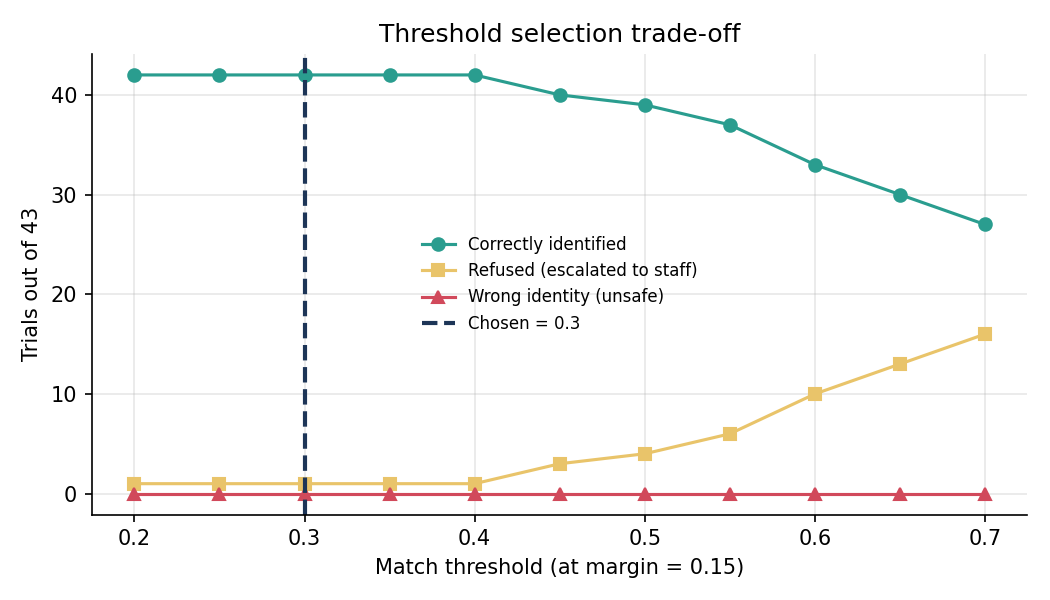
\includegraphics[width=0.86\textwidth]{03_threshold_sweep.png}
  \caption[Match-threshold selection trade-off]{Outcome of every probe
  as the match threshold is varied, at the deployed margin of $0.15$.
  This sweep was run on the calibration dataset as it stood before the
  loader defect was corrected (16 identities, 43 probes); the accuracy
  figures that follow use the corrected dataset (17 identities, 45
  probes).}
  \label{fig:threshold-sweep}
\end{figure}

The margin was first set at $0.10$. A sweep over enrolled probes could
not test the case that matters most --- a person who is not enrolled at
all --- so the open-set test described in
Section~\ref{subsec:heldout-accuracy} was added. It found one
non-enrolled person accepted as an enrolled student with a margin of
$0.110$, clearing $0.10$ by a hundredth. Across the corrected dataset,
genuine probes led their runner-up by at least $0.222$ (excluding the
one probe refused at every setting), while strangers led by at most
$0.110$. The margin was therefore raised to $0.15$, which lies between
the two with room on both sides and costs no genuine match.
Table~\ref{tab:calibrated-params} lists the calibrated values.

\begin{table}[H]
\centering
\caption{Calibrated recognition parameters.}
\label{tab:calibrated-params}
\begin{tabular}{llp{0.5\textwidth}}
\hline
Parameter & Value & Basis \\
\hline
$\tau_{\mathrm{match}}$ & $0.30$ & Below the lowest genuine score
  ($0.321$); no wrong identity at any threshold tested \\
$\tau_{\mathrm{margin}}$ & $0.15$ & Between the highest stranger
  margin ($0.110$) and the lowest genuine margin ($0.222$) \\
$\tau_{\mathrm{det}}$ & $0.60$ & Minimum face-detector confidence
  before a face is embedded \\
Embedding model & \texttt{buffalo\_s} & Fits the 512~MB deployment
  limit (98.9~MB loaded) \\
\hline
\end{tabular}
\end{table}

\subsection{Recognition Accuracy on Held-Out Probes}
\label{subsec:heldout-accuracy}

\textbf{Embedding quality.} Before any threshold is applied, the model
separates genuine from impostor pairs almost completely
(Table~\ref{tab:embedding-quality}). The area under the ROC curve is
$0.999907$; it is reported to six decimals deliberately, because at
four it prints as $1.0000$ and would read as perfect separation, when
the set in fact contains one inverted pair. The Equal Error Rate is
$0.42\%$, reached at a threshold of $0.320$ --- close to the deployed
$0.30$, which was chosen independently in
Section~\ref{subsec:calibration}.

\begin{table}[H]
\centering
\caption{Threshold-independent embedding quality ($N = 765$
comparisons).}
\label{tab:embedding-quality}
\begin{tabular}{lr}
\hline
Metric & Value \\
\hline
ROC AUC & $0.999907$ \\
Equal Error Rate & $0.42\%$ (at $0.320$) \\
Separation ($d'$) & $4.99$ \\
Genuine score, mean $\pm$ SD & $0.695 \pm 0.140$ \\
Impostor score, mean $\pm$ SD & $0.108 \pm 0.090$ \\
\hline
\end{tabular}
\end{table}

\begin{figure}[!htbp]
  \centering
  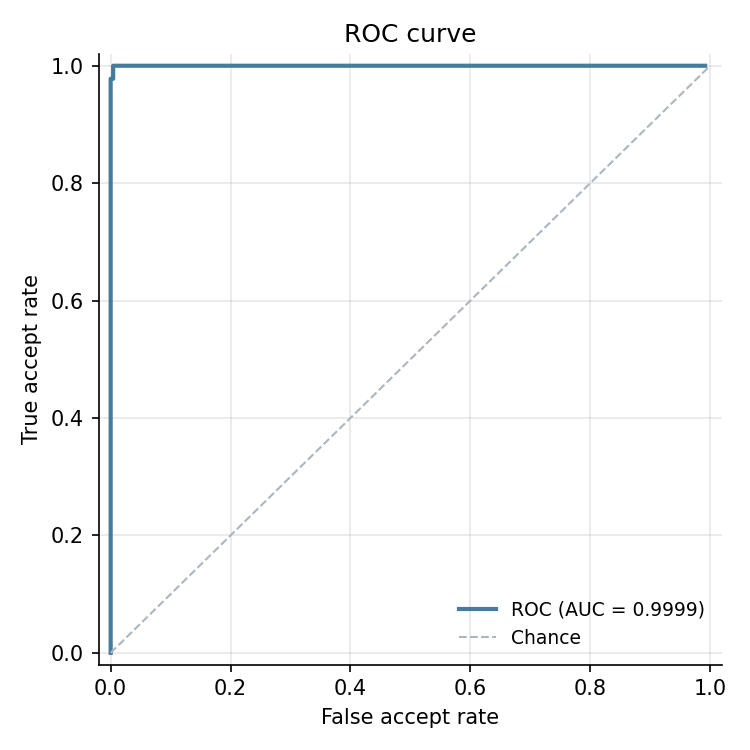
\includegraphics[width=0.62\textwidth]{07_roc_curve.png}
  \caption[ROC curve of the embedding model]{ROC curve over 45 genuine
  and 720 impostor pairs. AUC $= 0.999907$.}
  \label{fig:roc}
\end{figure}

\begin{figure}[!htbp]
  \centering
  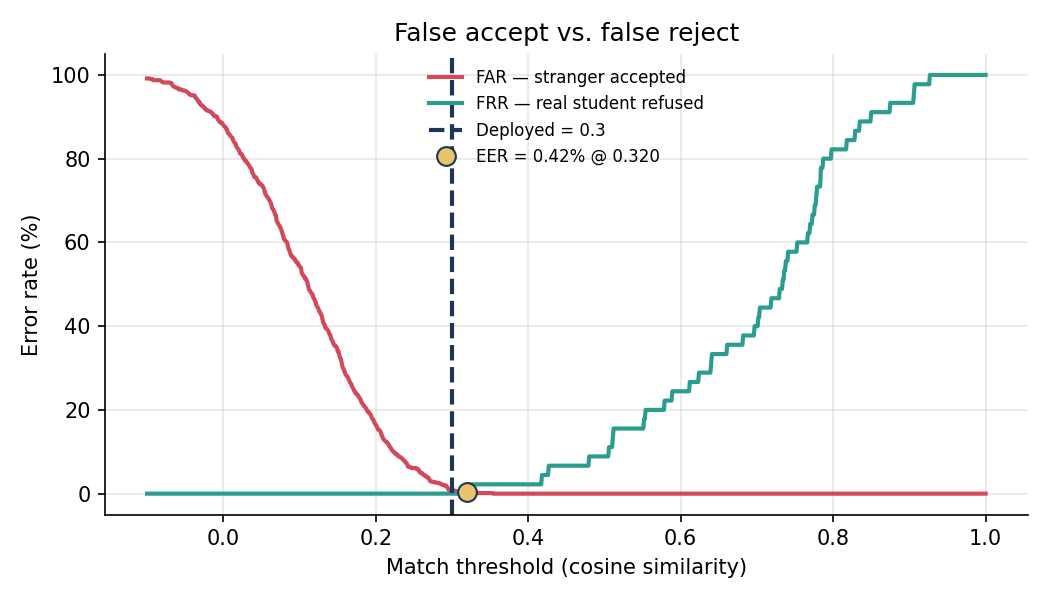
\includegraphics[width=0.9\textwidth]{06_far_frr.png}
  \caption[False accept and false reject rates]{False Accept Rate and
  False Reject Rate as the match threshold varies. The two cross at
  $0.42\%$ (EER, threshold $0.320$); the deployed threshold of $0.30$
  is marked.}
  \label{fig:far-frr}
\end{figure}

\begin{figure}[!htbp]
  \centering
  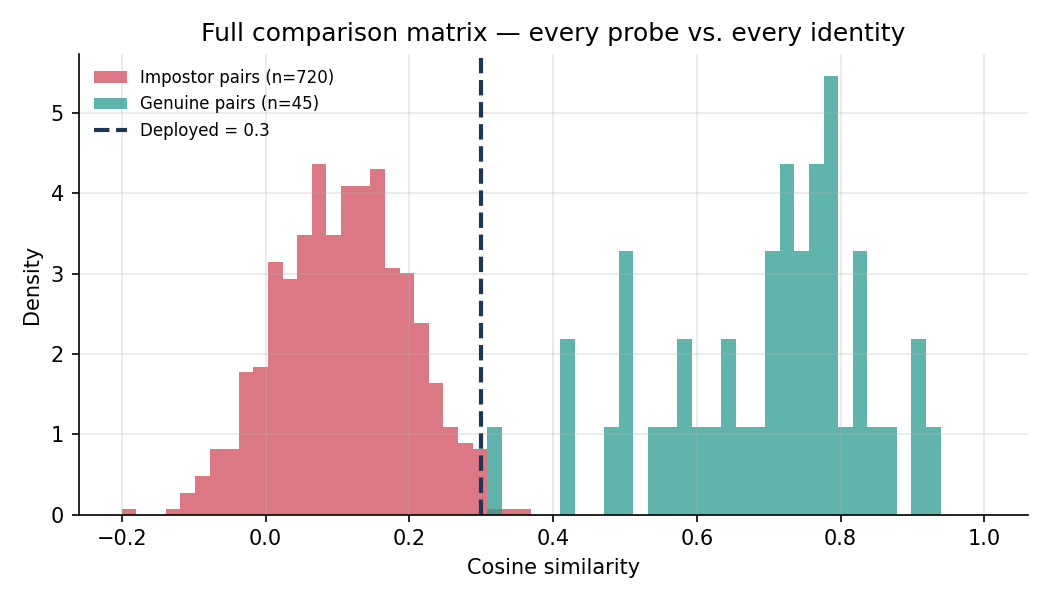
\includegraphics[width=0.9\textwidth]{08_full_score_distribution.png}
  \caption[Genuine and impostor score distributions]{Cosine similarity
  of every probe against every enrolled identity. Impostor pairs
  ($n = 720$) and genuine pairs ($n = 45$) occupy largely separate
  ranges; the few impostor pairs above $0.30$ are the cases the margin
  requirement exists to catch.}
  \label{fig:score-distribution}
\end{figure}

\textbf{Identification at the deployed thresholds.}
Table~\ref{tab:identification-outcomes} gives the outcome of every probe
under the full decision rule, in the form of a confusion matrix: each
probe is either linked to the correct student, linked to a wrong one,
or refused and escalated to staff. The first row is the closed-set
test, in which every probe belongs to an enrolled student. The second
is the open-set test, in which each person is removed from the gallery
and probed with their own photographs, so that they arrive as a
stranger.

\begin{table}[H]
\centering
\caption{Identification outcomes at $\tau_{\mathrm{match}} = 0.30$,
$\tau_{\mathrm{margin}} = 0.15$.}
\label{tab:identification-outcomes}
\begin{tabular}{lcccc}
\hline
Probe & Correctly linked & Wrong identity & Refused & Total \\
\hline
Enrolled student & $44$ ($97.8\%$) & $0$ ($0\%$) & $1$ ($2.2\%$) & $45$ \\
Not enrolled (stranger) & --- & $0$ ($0\%$) & $45$ ($100\%$) & $45$ \\
\hline
\end{tabular}
\end{table}

\noindent The correct student was ranked first for all 45 enrolled
probes (rank-1 accuracy $100\%$), and 44 of them were linked
automatically. The single refusal scored $0.321$ against the correct
student, but its runner-up was only $0.027$ behind; the rule declined to
choose between two candidates it could not separate and escalated to
staff. That is the safe failure --- the student is delayed, not given
someone else's number --- and no probe produced the unsafe one.

\textbf{Why the margin requirement is necessary.} The highest stranger
score in the open-set test was $0.353$, above $\tau_{\mathrm{match}}$.
Five stranger probes cleared the match threshold, and a rule that
applied the threshold alone would have issued each of them an enrolled
student's queue number. Table~\ref{tab:margin-caught} lists them, with
identities anonymised.

\begin{table}[H]
\centering
\caption{Stranger probes that cleared the match threshold.}
\label{tab:margin-caught}
\begin{tabular}{llcc}
\hline
Stranger & Would have been accepted as & Score & Margin \\
\hline
Person A & Enrolled student 1 & $0.353$ & $0.046$ \\
Person B & Enrolled student 2 & $0.331$ & $0.110$ \\
Person B & Enrolled student 2 & $0.326$ & $0.056$ \\
Person C & Enrolled student 1 & $0.305$ & $0.012$ \\
Person C & Enrolled student 3 & $0.302$ & $0.015$ \\
\hline
\multicolumn{2}{l}{Threshold alone} & \multicolumn{2}{r}{5 false identifications} \\
\multicolumn{2}{l}{Threshold and margin} & \multicolumn{2}{r}{0 false identifications} \\
\hline
\end{tabular}
\end{table}

\noindent None of the five led its runner-up by the required $0.15$,
and all five were refused. This is the measured case for the decision
rule that is this study's contribution: the pretrained model supplies
the similarity scores, but it is the requirement of a clear lead over
the runner-up that prevents a stranger from being issued an enrolled
student's number.

These probes are posed, cooperative, close-up photographs, whereas a
live capture is a crop of a person standing at queue-zone distance. The
figures above should therefore be read as an upper bound on live
performance. The remainder of this section reports how the same rule
behaved at the deployed camera.

\subsection{Separation Between Enrolled Students}
\label{subsec:enrol-separation}

Before recognition accuracy can be interpreted, it is necessary to know
how distinguishable the enrolled population is. With nine students
enrolled, the thirty-six distinct pairs of stored enrolment embeddings
were compared using Equation~\ref{eq:cosine}. Table~\ref{tab:enrol-sep}
reports the resulting impostor distribution.

\begin{table}[H]
\centering
\caption{Cosine similarity between the enrolment embeddings of different
students ($n = 9$ students, 36 pairs).}
\label{tab:enrol-sep}
\begin{tabular}{lc}
\hline
Statistic & Value \\
\hline
Mean impostor similarity & $0.1611$ \\
Standard deviation       & $0.0869$ \\
Minimum                  & $-0.0427$ \\
Maximum                  & $0.3561$ \\
\hline
\end{tabular}
\end{table}

\noindent The mean of $0.1611$ sits well below the acceptance threshold
$\tau_{\mathrm{match}} = 0.30$, confirming that enrolled students are
generally well separated. The maximum is the consequential figure: one
pair of genuinely different students reaches $0.3561$, which
\emph{exceeds} the acceptance threshold. An absolute threshold applied on
its own would therefore admit a comparison between these two students as
a valid match, and the identity finally reported would be decided by
whichever score happened to be higher. This is the condition the margin
requirement in Equation~\ref{eq:face-decision} exists to detect.

\begin{figure}[!htbp]
  \centering
  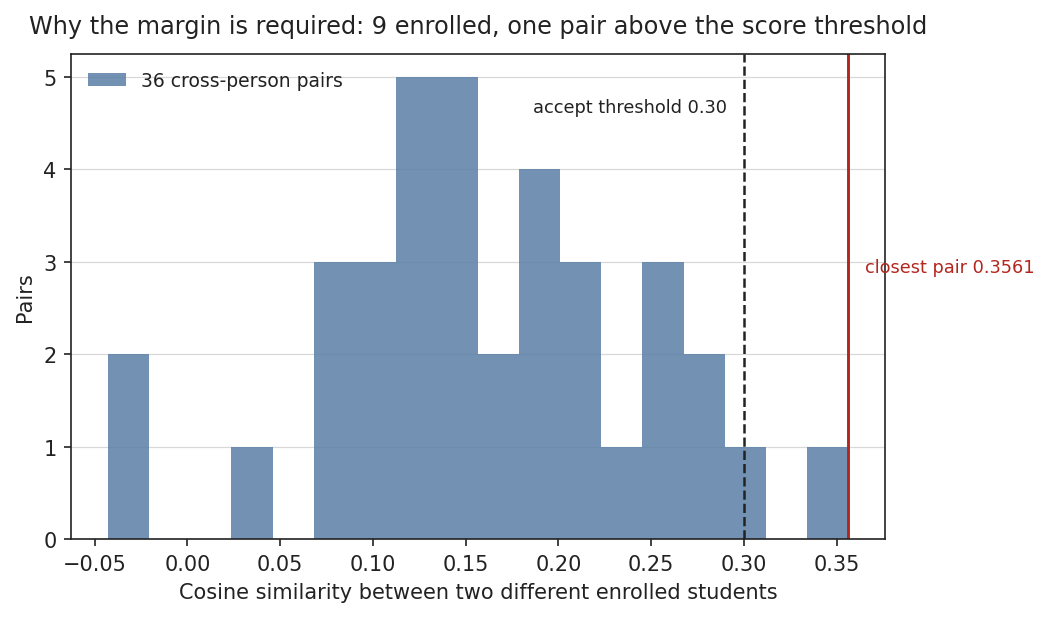
\includegraphics[width=0.86\textwidth]{sop2_03_impostor_separation.png}
  \caption[Similarity between different enrolled students]{Cosine
  similarity across all 36 pairs of different enrolled students. The
  closest pair exceeds the acceptance threshold, which is the situation an
  absolute threshold alone cannot resolve.}
  \label{fig:sop2-impostors}
\end{figure}

\subsection{Recognition Outcomes in Operation}
\label{subsec:recog-outcomes}

Every evaluation performed by Algorithm~4 is written to the recognition
audit table with its score, margin and outcome. Over the system-testing
period, 72 evaluations were logged. Of these, 45 came from the queue-zone
camera and 27 from the mobile client's face-login path, which uses the
same matcher and the same enrolled gallery but authenticates account
access rather than issuing a number. The camera evaluations are the ones
Statement of the Problem No.~2 concerns and are reported here; one is
excluded because it was recorded while only a single student was
enrolled, leaving no runner-up and therefore no meaningful margin.
Table~\ref{tab:recog-sep} summarises the remaining 44.

\begin{table}[H]
\centering
\caption{Score and margin ranges for accepted and refused queue-zone
recognitions ($N = 44$).}
\label{tab:recog-sep}
\begin{tabular}{lccc}
\hline
Outcome & $n$ & Score range & Margin range \\
\hline
Accepted & $18$ & $0.5408$--$0.7277$ & $0.2578$--$0.6823$ \\
Refused  & $26$ & $0.0780$--$0.2997$ & $0.0014$--$0.1492$ \\
\hline
Threshold & & $\tau_{\mathrm{match}} = 0.30$ & $\tau_{\mathrm{margin}} = 0.15$ \\
\hline
\end{tabular}
\end{table}

\noindent The two groups do not overlap on either criterion. The lowest
accepted score, $0.5408$, sits $0.2411$ above the highest refused score,
$0.2997$, and the lowest accepted margin, $0.2578$, sits $0.1087$ above
the highest refused margin, $0.1492$. Both thresholds fall inside those
gaps rather than near either boundary, so neither is finely tuned to the
observations. Figure~\ref{fig:sop2-decision} plots every evaluation
against the rule: the accepted and refused populations occupy separate
regions with an empty band between them, and the single refusal closest
to acceptance failed both conditions by less than $0.001$, which is the
behaviour a conservative rule should show at its boundary.

\begin{figure}[!htbp]
  \centering
  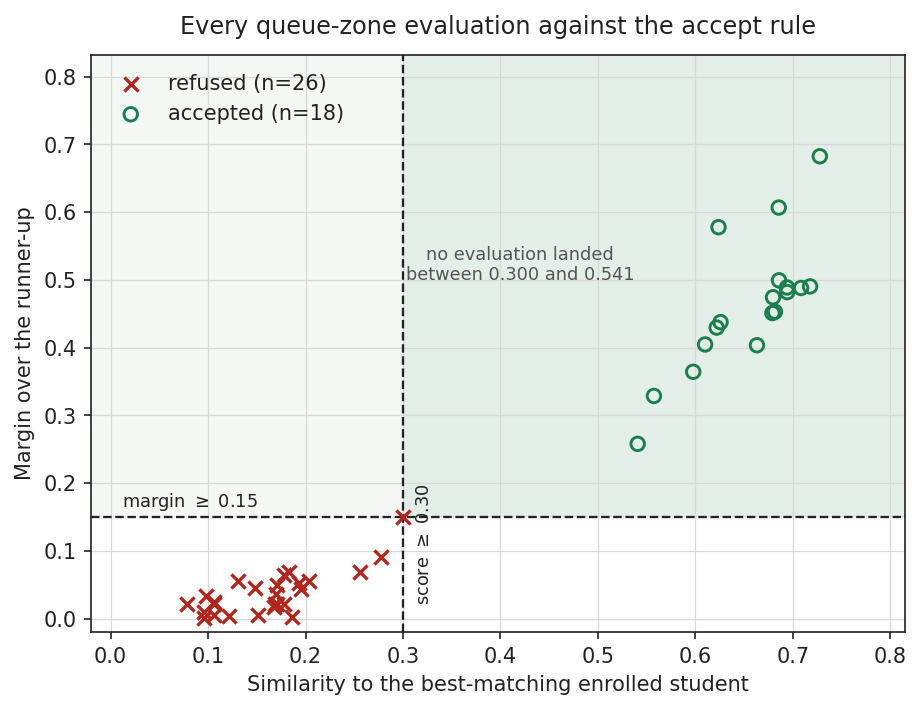
\includegraphics[width=0.86\textwidth]{sop2_01_decision_rule.png}
  \caption[Queue-zone evaluations against the accept rule]{Every
  queue-zone evaluation placed against the two-part accept rule. The
  shaded region is where both conditions hold. No evaluation fell between
  a score of $0.300$ and $0.541$.}
  \label{fig:sop2-decision}
\end{figure}

\begin{figure}[!htbp]
  \centering
  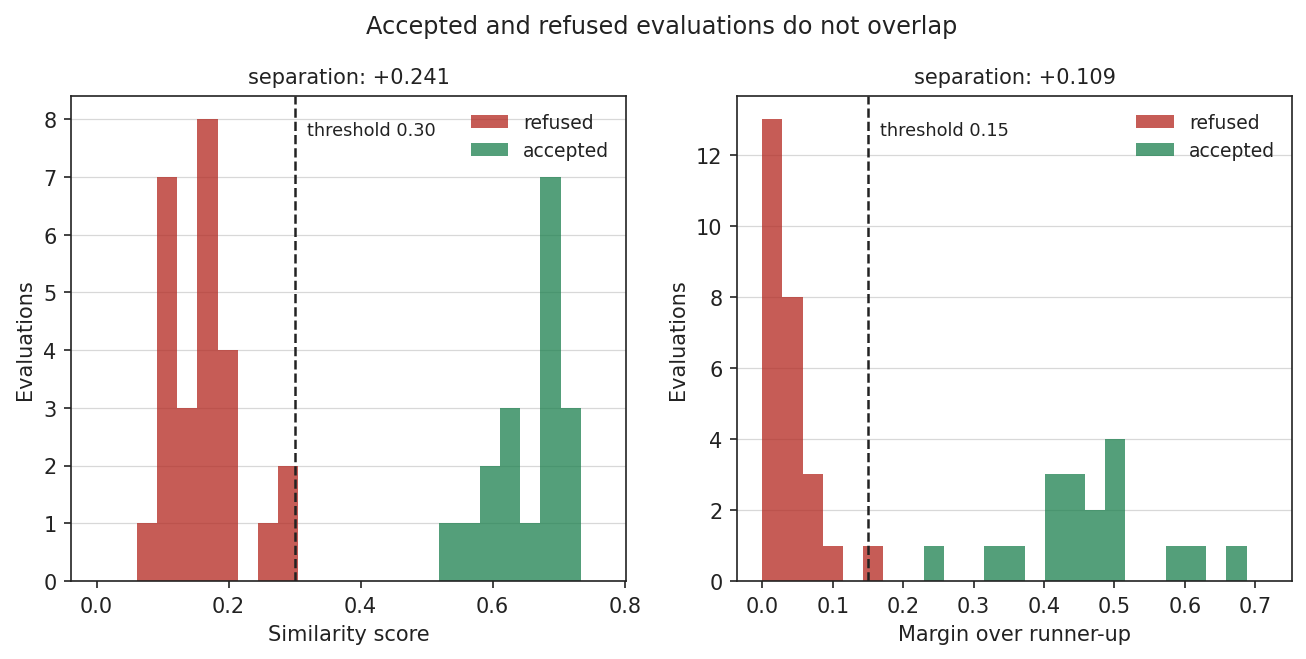
\includegraphics[width=\textwidth]{sop2_02_separation.png}
  \caption[Score and margin distributions by outcome]{Distributions of
  score and margin for accepted and refused queue-zone evaluations, with
  the deployed thresholds marked.}
  \label{fig:sop2-separation}
\end{figure}

\subsection{Evidence for the Margin Requirement}
\label{subsec:margin-evidence}

Because the audit table stores both the accepted score and its margin,
the runner-up similarity of every accepted recognition can be recovered
as $s^{(2)} = s^{(1)} - \mathrm{margin}$. This makes it possible to ask
how often the second-best candidate was itself above the acceptance
threshold, which is precisely the case an absolute threshold cannot
resolve.

The highest runner-up so far occurred on the face-login path, where the
system scored $0.7884$ against the correct student with a margin of
$0.4733$, placing the runner-up at $0.3150$. Two further evaluations on
that path produced runner-ups of $0.3096$ and $0.2997$. All three are at
or above $\tau_{\mathrm{match}} = 0.30$. Under a score-only rule, two
enrolled students would both have qualified for the same face, and the
system would have had to choose between them on a difference it had not
established as meaningful. The margin requirement resolved each case
without ambiguity.

That these occurred on the login path rather than at the camera does not
limit the finding. Both paths run the same matcher against the same
enrolled gallery, so how close two enrolled students can come is a
property of the roster, not of which camera is looking. The highest
runner-up recorded at the queue zone itself is $0.2830$, and the closest
pair of stored enrolment embeddings reaches $0.3561$
(Section~\ref{subsec:enrol-separation}), so the condition is reachable
there and has simply not yet been observed in the smaller number of
queue-zone evaluations.

The runner-up similarity also rises as the enrolled population grows. In
recognitions performed while two to four students were enrolled, the
runner-up ranged from $0.05$ to $0.14$; with eight or nine enrolled it
ranged from $0.23$ to $0.31$. This is the expected consequence of adding
identities to an open roster: each additional enrolment is another chance
that some enrolled face resembles the person at the camera. It also
indicates that an absolute threshold alone becomes progressively less
sufficient at the population sizes a campus deployment would reach, which
is the practical argument for the margin requirement rather than a higher
fixed threshold.

\subsection{Issuing the Queue Number Without Manual Input}
\label{subsec:sop2-issuance}

The second half of Statement of the Problem No.~2 concerns what follows a
successful identification: whether the queue number is issued without
manual input, and how quickly. Each issuance is recorded separately from
the recognition audit, with how the number was linked and the timestamps
around it.

Seven numbers were issued over the testing period. All seven were linked
by \texttt{face\_only}, the path in which the system mints the number
itself on an accepted match; none required a staff member to type a
number or a student to request one at the counter. Across the frames that
produced these seven issuances, the face-extraction stage returned a
usable embedding on 103 of 103 attempts.

Timing is reported in two consecutive phases, shown in
Figure~\ref{fig:sop2-issuance}. The first runs from the frame a person
first appears in to the moment their presence in the queue zone is
confirmed. The second runs from the moment the system was first able to
act --- the later of that confirmation and the student's join intent ---
to the number being issued, and averaged $4.80$~s across the seven.

The second phase is deliberately not measured from first sighting. With
the consent gate in place, a student may stand in frame for some time
before opening the app, and measuring from first sighting would charge
that waiting to the system: one run recorded $889$~s on that basis, which
is a person standing in front of the camera during unrelated work rather
than a recognition that took fifteen minutes. The raw timestamps remain
in the table, so any other interpretation can be recomputed.

\begin{figure}[!htbp]
  \centering
  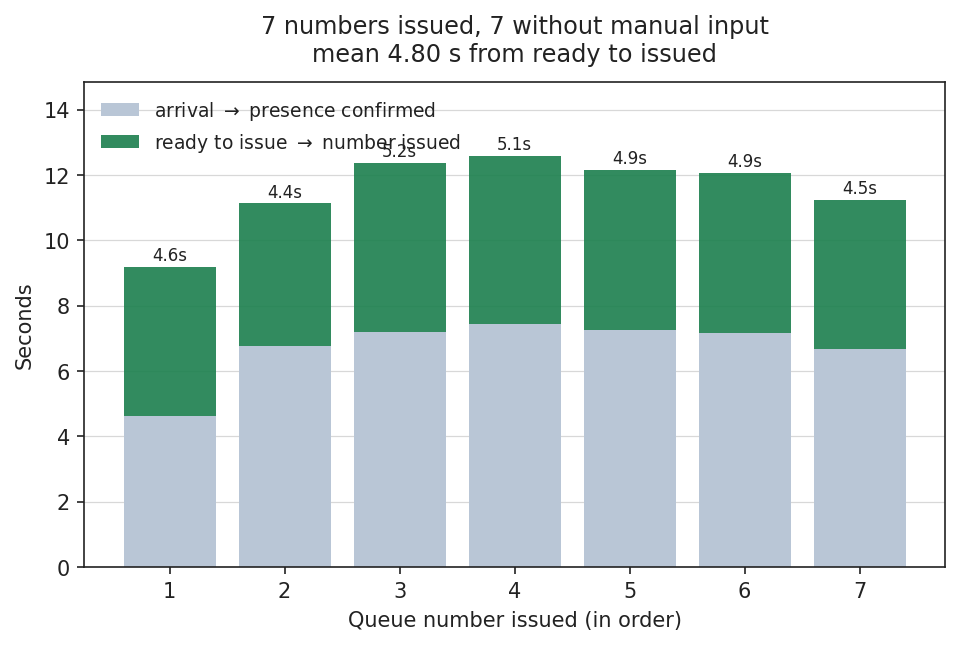
\includegraphics[width=0.86\textwidth]{sop2_04_issuance_time.png}
  \caption[Time from arrival to an issued queue number]{The two phases
  between a person arriving in the queue zone and holding a queue number,
  for each of the seven numbers issued. All seven were minted by the
  system without manual input.}
  \label{fig:sop2-issuance}
\end{figure}

\subsection{Load Testing}
\label{subsec:load-test}

As the panel recommended, the backend was load-tested to see whether it
stays responsive when many users poll it at once. The test used Locust
to simulate 50 concurrent users for two minutes across three user
classes --- students polling their queue status, the public display
board, and staff viewing analytics --- together with staff logins, against
a real seeded ticket rather than an invalid path. It was run against the
backend on the development machine, so it measures the application
itself and not the network path to the cloud deployment.
Table~\ref{tab:load-test} gives the results.

\begin{table}[H]
\centering
\caption{Backend response time under load (50 concurrent users,
2 minutes).}
\label{tab:load-test}
\begin{tabular}{lrrrr}
\hline
Endpoint & Median & 95th pct. & 99th pct. & Failures \\
\hline
Public display board & 7 ms & 13 ms & 46 ms & 0 \\
Wait-time prediction & 13 ms & 24 ms & 43 ms & 0 \\
Student queue status & 13 ms & 26 ms & 85 ms & 0 \\
Staff analytics & 21 ms & 36 ms & 50 ms & 0 \\
Staff login & 410 ms & 710 ms & 710 ms & 0 \\
\hline
\textbf{All requests} & \textbf{12 ms} & \textbf{31 ms} & \textbf{85 ms} &
  \textbf{0} \\
\hline
\end{tabular}
\end{table}

\noindent Across 2,536 requests at a sustained 21.3 requests per second,
none failed, and 95\% were answered within 31~ms. Staff login is slower
by design: passwords are hashed with a deliberately expensive function to
resist brute-force guessing, and because that work runs on its own
thread, the rest of the API held its 12~ms median while logins were in
progress. The limitation is the one stated above: a student or staff
member using the deployed system also waits for the round trip over the
internet to the cloud host, which this test does not include.

\subsection{Assessment of Statement of the Problem No.~2}
\label{subsec:sop2-scope}

Statement of the Problem No.~2 asks what level of accuracy the
face-recognition system reaches in identifying enrolled students and
assigning queue numbers without manual input. On held-out photographs
with known identities, the system linked $97.8\%$ of enrolled students
automatically, ranked the correct student first in every case, assigned
no one to a wrong identity, and refused every one of 45 non-enrolled
probes. In live operation at the queue-zone camera, every queue number
issued --- seven of seven --- was minted by the system without staff or
student input, with a mean of $4.80$~s from the moment the system could
act to the number being issued. The rule's defining property held in
both settings: when it could not identify someone with confidence, it
refused rather than guessed.

These findings must be interpreted with four limitations.

\begin{enumerate}
  \item \textbf{The offline figures are an upper bound.} The held-out
        probes are posed, close-up photographs. Live captures are person
        crops at queue-zone distance and score lower, so live accuracy
        should be expected to fall below the offline figures, most
        likely as more refusals rather than as wrong identities.
  \item \textbf{Live recognitions have no ground truth.} The live
        results in Sections~\ref{subsec:enrol-separation}
        to~\ref{subsec:sop2-issuance} come from the system's own record.
        They have not been checked against an independent observer's
        log, so the proportion of correct assignments over total
        arrivals and the re-identification reliability defined in
        Equation~\ref{eq:accuracy} remain to be measured during the
        evaluation period, together with the ticket and token validation
        rate and the detection-to-ticket latency.
  \item \textbf{The populations are small.} The offline evaluation
        covers 17 identities and the deployment nine enrolled students.
        Each additional enrolment adds another face that could resemble
        a new arrival, so the separation figures should be recomputed as
        enrolment grows.
  \item \textbf{No liveness check.} The system does not test whether
        the face in front of the camera belongs to a live person, so it
        cannot distinguish a student from a printed or on-screen
        photograph of that student.
\end{enumerate}

% ----------------------------------------------------------------
% 3.3  SOP #3 — Wait-time prediction accuracy (MAE and MAPE)
% ----------------------------------------------------------------
\section{Wait-Time Prediction Accuracy}
\label{sec:sop3-results}

This section addresses Statement of the Problem No.~3: \emph{What is
the level of accuracy of the system's wait-time prediction model in
terms of Mean Absolute Error (MAE) and Mean Absolute Percentage Error
(MAPE)?}

\subsection{Wait-Time Predictor Training Result}
\label{sec:wait-time-training-result}
After cleaning and wait-time reconstruction, the prepared dataset
contained 30,362 supervised rows. Applying the one-minute minimum-wait
filter left 19,119 modeling rows. The date-based split produced 13,031
training rows and 6,088 test rows. The training period covered
May~24,~2023 to January~20,~2026, and the test period covered
January~21,~2026 to May~4,~2026. On the test set, the Gradient
Boosting model obtained MAE~=~2.3512 minutes, RMSE~=~4.0858 minutes,
MAPE~=~80.74\%, and $R^2=-0.0349$. The MAE and RMSE are used as the
main accuracy indicators, while MAPE is reported with caution because
short reconstructed waits inflate percentage error.

% TODO: Insert live evaluation MAE and MAPE results here after the
% evaluation period. Report separately for the current, 5-minute,
% 15-minute, and 30-minute prediction horizons.

% ----------------------------------------------------------------
% 3.4  SOP #4 — User satisfaction (usability, reliability, clarity)
% ----------------------------------------------------------------
\section{User Satisfaction}
\label{sec:sop4-results}

This section addresses Statement of the Problem No.~4: \emph{What is
the level of user's satisfaction in terms of system's usability,
system's reliability, and system clarity?} Results are reported per
dimension and per respondent group using the weighted mean and overall
weighted mean, interpreted against the Likert scale in
Table~\ref{tab:likert}. The responses come from the supervised trial
session under the shortened evaluation protocol described in
Section~\ref{sec:datagathering}, and describe users' first experience of
the system rather than satisfaction after sustained use.

% TODO: Insert weighted mean tables and interpretation here after the
% post-evaluation survey is administered and analyzed.

% ----------------------------------------------------------------
% 3.5  Summary of Findings
% ----------------------------------------------------------------
\section{Summary of Findings}
\label{sec:summary-findings}

% TODO: Summarize key findings across all four SOP responses once
% evaluation data are collected and analyzed.

% ============================================================
% APPENDIX A: SYNTHESIS MATRIX
% ============================================================
\appendix
\refstepcounter{chapter}
\setcounter{section}{0}
\setcounter{table}{0}
\addcontentsline{toc}{chapter}{Appendix \thechapter: Synthesis Matrix of Related Literature}
\section*{Appendix \thechapter: Synthesis Matrix of Related Literature}
\label{app:synthesis-matrix}

Table~\ref{tab:synthesis} presents a synthesis matrix summarizing the
reviewed literature, the methodology of each study, key findings, and
the gaps identified that motivated the present work.

\begin{table}[H]
  \caption{Synthesis Matrix of Related Literature}
  \label{tab:synthesis}
  \centering
  \scriptsize
  \setlength{\tabcolsep}{3pt}
  \renewcommand{\arraystretch}{1.02}
  \begin{tabular}{p{2.7cm} c p{3.0cm} p{3.3cm} p{3.7cm}}
    \toprule
    \textbf{Author/s} & \textbf{Year} & \textbf{Topic/Focus} &
    \textbf{Findings} & \textbf{Gap/Limitation} \\
    \midrule
    Sindagi \& Patel~\cite{sindagi2018survey} & 2018 &
      CNN-based crowd counting and density estimation &
      Deep learning enables robust counting under occlusion and scale variation &
      No queue-number assignment or re-identification \\[0.3em]
    Redmon \& Farhadi~\cite{redmon2018} & 2018 &
      YOLOv3 real-time object detection &
      Single-pass network predicts bounding boxes and class probabilities &
      No queue-specific deduplication \\[0.3em]
    Jocher et al.~\cite{jocher2023} & 2023 &
      YOLOv8 multi-scale anchor-free detection &
      Accuracy-speed tradeoff with persistent tracking support &
      Duplicate head/body boxes in close-range scenarios \\[0.3em]
    Wang et al.~\cite{wang2025lightweight} & 2025 &
      Lightweight YOLOv8n-derived person detector &
      Supports edge-device surveillance person detection with reduced overhead &
      Surveillance-focused; no queue ticketing or wait-time prediction \\[0.3em]
    Jocher \& Qiu~\cite{jocher2024yolo11} & 2024 &
      YOLO11 object detection software &
      Improves model efficiency and feature reuse in the Ultralytics family &
      Newer variant; not selected for stable prototype integration \\[0.3em]
    Tian et al.~\cite{tian2025yolov12} & 2025 &
      Attention-centric YOLOv12 detector &
      Introduces attention-oriented architecture for real-time detection &
      Benchmark-focused; added complexity for campus prototype hardware \\[0.3em]
    Terven et al.~\cite{terven2023yolo} & 2023 &
      Comprehensive review of YOLO architectures &
      Documents innovations from YOLOv1 to YOLOv8 and YOLO-NAS &
      General review; no queue-specific application \\[0.3em]
\bottomrule
  \end{tabular}
\end{table}

\begin{center}
\scriptsize
\setlength{\tabcolsep}{3pt}
\renewcommand{\arraystretch}{1.02}
\textbf{Table~\ref{tab:synthesis} continued}\\[0.2em]
\begin{tabular}{p{2.7cm} c p{3.0cm} p{3.3cm} p{3.7cm}}
  \toprule
  \textbf{Author/s} & \textbf{Year} & \textbf{Topic/Focus} &
  \textbf{Findings} & \textbf{Gap/Limitation} \\
  \midrule
    Wojke et al.~\cite{wojke2017deepsort} & 2017 &
      DeepSORT online multi-object tracking &
      Appearance and motion association reduce identity switches during occlusion &
      No explicit queue-position semantics \\[0.3em]
    Ye et al.~\cite{ye2022reid} & 2022 &
      Deep learning for person re-identification &
      Categorizes feature learning, metric learning, and ranking approaches &
      No integration with queue management \\[0.3em]
    Wang et al.~\cite{wang2024reid} & 2024 &
      Person and vehicle re-identification survey &
      Reviews recent Re-ID advances and robustness challenges &
      Broader Re-ID scope; no campus queue workflow \\[0.3em]
    Asperti et al.~\cite{asperti2025reid} & 2025 &
      Recent person re-identification techniques &
      Documents newer representation and robustness approaches &
      Deep Re-ID methods add overhead for a single-zone prototype \\[0.3em]
    Padilla-Lopez et al.~\cite{padillalopez2015privacy} & 2015 &
      Visual privacy protection methods &
      Categorizes anonymization, scrambling, and aggregation techniques &
      Not specific to queue or service-area monitoring \\[0.3em]
    Concepcion et al.~\cite{concepcion2026smart} & 2026 &
      Smart queuing and appointment system in a Philippine HEI &
      Web-based queue and appointment management can improve client services &
      User-initiated ticketing; no passive computer-vision arrival detection \\[0.3em]
    Shortle et al.~\cite{shortle2018fundamentals} & 2018 &
      Foundational queueing theory &
      M/M/c and Little's Law enable wait-time calculation &
      No integration with CV inputs \\[0.3em]
    Holt~\cite{holt2004forecasting} & 2004 &
      Exponentially weighted moving average forecasting &
      Trend and level smoothing capture short-term dynamics &
      No queue-specific application \\[0.3em]
    Shmueli \& Koppius~\cite{shmueli2011predictive} & 2011 &
      Predictive analytics as a research paradigm &
      Empirical prediction supports decision-making &
      Not applied to live queue systems \\[0.3em]
    Hyndman \& Athanasopoulos~\cite{hyndman2021forecasting} & 2021 &
      Forecasting principles and practice &
      Treats exponential smoothing and multi-horizon forecasting &
      Not domain-specific to service queues \\
  \bottomrule
\end{tabular}
\end{center}

\clearpage
\chapter{Baseline Questionnaire on the Current Queue Process}
\label{app:sop1-questionnaire}

This instrument addresses Statement of the Problem No.~1 and was
administered before deployment. It has a staff form and a student form
answered against the same five-point scale (5 = Strongly Agree,
1 = Strongly Disagree). Every item states a problem; agreement means the
problem is present.

\section*{Staff / Cashier Form}

\noindent\textbf{Profile.} (1)~How long have you been handling queue
transactions in this office? (2)~On average, how often do you
personally handle queue management during busy periods?

\medskip
\noindent\textbf{Perceived problems on wait-time}
\begin{enumerate}
  \item The current display only shows the number being served, not how
        long a client still needs to wait.
  \item It is difficult to predict how long a client will wait after
        receiving their paper ticket.
  \item Wait times increase significantly during peak or busy periods.
  \item Wait times increase further when a window is closed or on break,
        since queue numbers are not redistributed to open windows.
  \item It is difficult to manage the queue efficiently when a window
        has to close temporarily during busy periods.
  \item No-show clients disrupt the flow of the numbering system.
  \item There is no way to notify clients in advance that their number
        is about to be called.
\end{enumerate}

\noindent\textbf{Perceived problems on user experience}
\begin{enumerate}
  \item Clients frequently approach the counter to ask about their
        number or wait time.
  \item Clients get confused when a window shows no number, since the
        display does not indicate whether it is closed, on break, or not
        yet in use.
  \item It is difficult to manage complaints related to long or unclear
        wait times.
  \item Handling paper tickets creates additional workload for staff
        during busy periods.
  \item It is challenging to maintain order in the queue area during
        busy periods despite having a numbering system.
  \item Miscommunication with clients occurs when the display and the
        actual queue status do not match.
  \item Overall, the current queue system negatively affects the quality
        of service provided to clients.
\end{enumerate}

\noindent\textbf{Open-ended.} In your own words, what is the biggest
problem you experience with the current queue process?

\section*{Student Form}

\noindent\textbf{Profile.} (1)~Year level. (2)~How often do you avail of
services that require queuing during busy periods?

\medskip
\noindent\textbf{Perceived problems on wait-time}
\begin{enumerate}
  \item The display screen only shows the number currently being served,
        not how long I still need to wait.
  \item I have experienced long wait times when transacting during busy
        periods.
  \item I have no way of knowing my estimated wait time after getting my
        paper ticket.
  \item I need to keep watching the display screen to know when my
        number will be called.
  \item I have missed my turn because I was not near the display when my
        number was called.
  \item Waiting time feels unpredictable, especially during busy periods.
  \item Long or unpredictable wait times discourage me from availing
        certain services during peak hours.
\end{enumerate}

\noindent\textbf{Perceived problems on user experience}
\begin{enumerate}
  \item I find it inconvenient that I have to physically watch the
        screen or ask staff to know my queue status.
  \item I get confused about whether a window is closed, on break, or
        just not yet available when its display shows no number.
  \item I feel frustrated when I do not know how many people are still
        ahead of me.
  \item There is no notification or alert to tell me when my turn is
        near.
  \item I find it inconvenient to wait without knowing how much time is
        left.
  \item The lack of a wait-time estimate affects my overall experience
        in transacting at the office.
  \item Overall, I am dissatisfied with the current queue management
        process.
\end{enumerate}

\noindent\textbf{Open-ended.} In your own words, what is the biggest
problem you experience while waiting in line at this office?

\clearpage
\chapter{\sysname{} Evaluation Questionnaire}
\label{app:queueflow-questionnaire}

\begin{center}
\textbf{FOR CONTENT VALIDATION -- DRAFT}\\[0.5em]
\textbf{Naga College Foundation, Inc. -- College of Computer Studies}\\[1em]
\textbf{Research Title:} \sysname{}: A Computer Vision-Based Smart Queue
Management and Predictive Service Delivery System\\[0.5em]
\textbf{Researchers:} Archie D. Balbin and Joshua Rovic P. Sanota
\end{center}

\section*{Pre-Screening}

Are you 18 years of age or older?

\noindent $\square$ Yes \hspace{2em} $\square$ No

\noindent Respondents who answer No are thanked and are not included in
the study. No profile answers or survey responses are collected from
them.

\section*{Section I: Respondent Profile}

\begin{enumerate}
  \setlength{\itemsep}{1pt}
  \item Respondent code assigned by researchers:
        \rule{0.45\textwidth}{0.4pt}
  \item Respondent group:
        $\square$ Cashier Staff \quad
        $\square$ Student
  \item For students only -- Year level:
        $\square$ 1st year \quad
        $\square$ 2nd year \quad
        $\square$ 3rd year \quad
        $\square$ 4th year \quad
        $\square$ 5th year or above
  \item For students only -- How did you receive your queue number
        during the session?\\
        $\square$ Automatically, after the camera recognised me \quad
        $\square$ From staff, because the system could not recognise me
\end{enumerate}

\section*{Instructions}

Answer only the form for your group: students answer Section~II, and
cashier staff answer Section~III. For each statement, choose
the box that best matches your experience with \sysname{} during the
trial session.

\medskip
\noindent\textbf{Rating scale:} 5 = Strongly Agree \quad 4 = Agree \quad
3 = Neutral \quad 2 = Disagree \quad 1 = Strongly Disagree

\providecommand{\ratingbox}{\ensuremath{\square}}
\newcommand{\rb}{\ratingbox & \ratingbox & \ratingbox & \ratingbox & \ratingbox}

\clearpage
\section*{Section II: Student Form}

\begin{table}[H]
\small
\caption{Student form (15 items).}
\label{tab:appb-student}
\centering
\renewcommand{\arraystretch}{1.12}
\begin{tabular}{p{0.9cm} p{9.3cm} c c c c c}
\toprule
\textbf{Code} & \textbf{Statement} &
\textbf{5} & \textbf{4} & \textbf{3} & \textbf{2} & \textbf{1} \\
\midrule
\multicolumn{7}{l}{\textit{A.\ System's usability}} \\
U1 & The system was easy to use without needing someone to guide me. & \rb \\
U2 & I was able to complete what I needed to do without difficulty. & \rb \\
U3-s & Registering my face in the mobile app was easy. & \rb \\
U4-s & Asking to be queued from the mobile app was convenient. & \rb \\
U5-s & I received my queue number without having to do anything else at
  the office. & \rb \\
\midrule
\multicolumn{7}{l}{\textit{B.\ System's reliability}} \\
R1 & The system worked consistently throughout the session. & \rb \\
R2 & I did not encounter errors that stopped me from continuing. & \rb \\
R3-s & The system recognised me correctly when I entered the queue area. & \rb \\
R4-s & I trust that the queue number I received was mine and not someone
  else's. & \rb \\
R5-s & My position in the queue was updated correctly as the line moved. & \rb \\
\midrule
\multicolumn{7}{l}{\textit{C.\ System clarity}} \\
C1 & The information shown on screen was easy to understand. & \rb \\
C2 & I always knew what the system was doing or waiting for. & \rb \\
C3-s & My position in the queue was clearly shown. & \rb \\
C4-s & The estimated waiting time was presented in a way I could
  understand. & \rb \\
C5-s & I understood what information the system keeps about me. & \rb \\
\bottomrule
\end{tabular}
\end{table}

\clearpage
\section*{Section III: Cashier Staff Form}

\begin{table}[H]
\small
\caption{Cashier staff form (15 items).}
\label{tab:appb-staff}
\centering
\renewcommand{\arraystretch}{1.12}
\begin{tabular}{p{0.9cm} p{9.3cm} c c c c c}
\toprule
\textbf{Code} & \textbf{Statement} &
\textbf{5} & \textbf{4} & \textbf{3} & \textbf{2} & \textbf{1} \\
\midrule
\multicolumn{7}{l}{\textit{A.\ System's usability}} \\
U1 & The system was easy to use without needing someone to guide me. & \rb \\
U2 & I was able to complete what I needed to do without difficulty. & \rb \\
U3-f & Navigating the staff dashboard was easy. & \rb \\
U4-f & Marking an entry as done or as a no-show was quick to do. & \rb \\
U5-f & When the system could not identify someone, resolving it from the
  dashboard was straightforward. & \rb \\
\midrule
\multicolumn{7}{l}{\textit{B.\ System's reliability}} \\
R1 & The system worked consistently throughout the session. & \rb \\
R2 & I did not encounter errors that stopped me from continuing. & \rb \\
R3-f & The queue numbers the system issued matched the students actually
  present. & \rb \\
R4-f & When the system was unsure about someone, it referred them to staff
  instead of guessing. & \rb \\
R5-f & The queue list on the dashboard stayed accurate as students were
  served. & \rb \\
\midrule
\multicolumn{7}{l}{\textit{C.\ System clarity}} \\
C1 & The information shown on screen was easy to understand. & \rb \\
C2 & I always knew what the system was doing or waiting for. & \rb \\
C3-f & The dashboard layout made it easy to find what I needed. & \rb \\
C4-f & The live camera view and the queue list were clear to read. & \rb \\
C5-f & The wait-time predictions and analytics were presented in a way I
  could act on. & \rb \\
\bottomrule
\end{tabular}
\end{table}

\section*{Section IV: Additional Questions (not scored)}

\begin{enumerate}
  \item Did the system ever fail to recognise you, or give you a number
        you did not expect?
        $\square$ No \quad $\square$ Yes, once \quad
        $\square$ Yes, more than once
  \item If yes, what happened?\\[0.3em]
        \rule{\linewidth}{0.4pt}
  \item How comfortable are you with the system using your face to
        identify you in the queue?\\
        $\square$ Very comfortable \quad $\square$ Comfortable \quad
        $\square$ Neutral \quad $\square$ Uncomfortable \quad
        $\square$ Very uncomfortable
  \item What did you like most about \sysname{}?\\[0.3em]
        \rule{\linewidth}{0.4pt}
  \item If you could change one thing about \sysname{}, what would it
        be?\\[0.3em]
        \rule{\linewidth}{0.4pt}
\end{enumerate}

\begin{center}
\textbf{End of Questionnaire.} Thank you for your participation.
\end{center}

\section*{Questionnaire Notes}

Each respondent answers fifteen items, five in each dimension of
Statement of the Problem No.~4. Two items in every dimension (U1--U2,
R1--R2, C1--C2) are common to both forms, so that students and staff
can be compared on the same statements; the other three are specific to
the respondent's role, since a student cannot judge the staff dashboard
and a staff member cannot judge the mobile application. Every statement
is worded so that agreement is favourable, so no item needs
reverse-scoring.

Weighted means are computed per item, per dimension, and per group as
described in Section~2.7. Under the shortened evaluation protocol, the
questionnaire is content-validated by three expert raters in a single
review round before use, and its internal consistency is measured with
Cronbach's alpha on the responses themselves rather than on a separate
pilot sample. The questions in Section~IV are reported descriptively and
do not enter any weighted mean.


% ============================================================
% BIBLIOGRAPHY
% ============================================================
\printbibliography

\end{document}
